\documentclass[a4paper, 12pt, openany]{book}
\usepackage[utf8]{inputenc}
\usepackage[english]{babel}

% page layout
\usepackage[left=15mm, right=15mm, top=25mm]{geometry}
\geometry{a4paper}

% images
\usepackage{graphicx}

% headers and foooters
\usepackage{fancyhdr}
\setlength{\headheight}{15pt}

% part name
\let\Oldpart\part
\newcommand{\parttitle}{}
\renewcommand{\part}[1]{\Oldpart{#1}\renewcommand{\parttitle}{#1}}

% no random page numbers
\fancypagestyle{plain}{%
  \fancyhf{}                          % clear all header and footer fields
  \renewcommand{\headrulewidth}{0pt}
  \renewcommand{\footrulewidth}{0pt}
}

% custom headers and footers
\renewcommand{\chaptermark}[1]{\markboth{#1}{#1}}
\pagestyle{fancy}
\fancyhead{}
\fancyfoot{}

\fancypagestyle{body}{%
  \fancyhead[LE,RO]{\thepage}%
  \fancyhead[LO]{\chaptername\ \thechapter:\ \leftmark}%
  \fancyhead[RE]{\partname\ \thepart:\ \parttitle}%
}

% special header for Introduzione
\fancypagestyle{introd}{%
  \fancyhead[LE,RO]{\thepage}%
  \fancyhead[RE,LO]{\leftmark}%
}

% special header for Indice
\fancypagestyle{indice}{%
  \fancyhead[LE,RO]{\thepage}%
  \fancyhead[RE,LO]{Indice}%
}

% special header for Contents
\fancypagestyle{contents}{%
  \fancyhead[LE,RO]{\thepage}%
  \fancyhead[RE,LO]{Contents}%
}

% no blank pages
\let\cleardoublepage\clearpage
% removes indentation
\setlength{\parindent}{0pt}
% add subsubsection numbering
\setcounter{secnumdepth}{3}

% math
\usepackage{amsmath}
\usepackage{amssymb}
\usepackage{amsfonts}
\usepackage{amsthm}
\usepackage{mathtools}
\usepackage{mathrsfs}
\usepackage{tensor}

% physics
\usepackage{braket}

% chemistry
\usepackage{chemformula}

% custom environments
%\newtheoremstyle{theorem}{}{}{\slshape}{}{\bfseries}{.}{ }{}

%\theoremstyle{definition}
%\newtheorem{definition}{Definition}[section]

%\theoremstyle{theorem}
%\newtheorem{theorem}{Theorem}[section]

%\theoremstyle{theorem}
%\newtheorem{corollary}{Corollary}[theorem]

%\theoremstyle{theorem}
%\newtheorem{lemma}{Lemma}[section]

%\theoremstyle{theorem}
%\newtheorem{lemcorollary}{Corollary}[lemma]

%\theoremstyle{theorem}
%\newtheorem{proposition}{Proposition}[section]

%\theoremstyle{theorem}
%\newtheorem{propcorollary}{Corollary}[proposition]

%\theoremstyle{remark}
%\newtheorem{example}{Example}[section]

% fancy environments
\usepackage[many]{tcolorbox}
\tcbuselibrary{theorems}

\NewTcbTheorem[number within=section]{definition}{Definition}%
{enhanced, breakable, colback=green!5, colframe=green!35!black, fonttitle=\bfseries}{def}

\newtcbtheorem[number within=section]{theorem}{Theorem}%
{enhanced, breakable, colback=red!5, colframe=red!35!black, fonttitle=\bfseries}{th}

\newtcbtheorem[number within=tcb@cnt@theorem]{corollary}{Corollary}%
{enhanced, breakable, colback=red!5, colframe=red!35!black, fonttitle=\bfseries}{cor}

\newtcbtheorem[number within=section]{lemma}{Lemma}%
{enhanced, breakable, colback=blue!5, colframe=blue!35!black, fonttitle=\bfseries}{lemma}

\newtcbtheorem[number within=lemma]{lemcorollary}{Corollary}%
{enhanced, breakable, colback=blue!5, colframe=blue!35!black, fonttitle=\bfseries}{cor}

\newtcbtheorem[number within=section]{proposition}{Proposition}%
{enhanced, breakable, colback=cyan!5, colframe=cyan!35!black, fonttitle=\bfseries}{prop}

\newtcbtheorem[number within=proposition]{propcorollary}{Corollary}%
{enhanced, breakable, colback=cyan!5, colframe=cyan!35!black, fonttitle=\bfseries}{cor}

\newtcbtheorem[number within=section]{example}{Example}%
{enhanced, breakable, colback=yellow!5, colframe=yellow!35!black,fonttitle=\bfseries}{ex}

% sectioning
\usepackage{titlesec}

% hyper-references
\usepackage{hyperref}

% extended integral symbols
\usepackage{esint}

% add table of contents, index and bibliography to table of contents
\usepackage{tocbibind}

% text
\newcommand{\virgolette}[1]{``\text{#1}"}
\newcommand{\tildetext}{\raise.17ex\hbox{$\scriptstyle\mathtt{\sim}$}}

% greek
\newcommand{\Chi}{\text{X}}

% custom math symbols
\newcommand{\abs}[1]{\left\lvert#1\right\rvert}
\newcommand{\norm}[1]{\left\lVert#1\right\rVert}
\newcommand{\sgn}[1]{\mathrm{sgn}\,#1}
\newcommand{\pa}{\partial}
\newcommand{\na}{\nabla}
\newcommand{\tens}[1]{\mathrm{#1}}
\newcommand{\defeq}{\mathrel{\vcenter{\baselineskip0.5ex \lineskiplimit0pt
                     \hbox{\scriptsize.}\hbox{\scriptsize.}}}%
                     =}
\newcommand{\eqdef}{=%
                     \mathrel{\vcenter{\baselineskip0.5ex \lineskiplimit0pt
                     \hbox{\scriptsize.}\hbox{\scriptsize.}}}}
\newcommand{\ve}[1]{\mathbf{#1}}
\newcommand{\lap}{\triangle}
\newcommand{\hilb}{\mathscr{H}}
\DeclareMathOperator{\diag}{diag}
\newcommand{\sqg}{\sqrt{\tens{g}}}
\newcommand{\sqgm}{\sqrt{-\tens{g}}}
\newcommand{\cm}{\mathcal{C}^{\infty}(\mathcal{M})}
\DeclareMathOperator{\lspan}{span}
\newcommand{\xm}{\mathfrak{X}(\mathcal{M})}
\DeclareMathOperator{\id}{id}
\newcommand{\ld}{\mathcal{L}}
\newcommand{\lm}[1]{\Lambda^{#1}(\mathcal{M})}
\newcommand{\hrm}[1]{\mathrm{Harm}^{#1}(\mathcal{M})}
\DeclareMathOperator{\ran}{ran}
\DeclareMathOperator{\tr}{tr}
\DeclareMathOperator{\End}{End}
\DeclareMathOperator{\im}{Im}
\newcommand{\dd}{\mathrm{d}}
\newcommand{\bs}[1]{\boldsymbol{#1}}

% small \overleftrightarrow
\makeatletter
\newcommand{\overleftrightsmallarrow}{\mathpalette{\overarrowsmall@\leftrightarrowfill@}}
\newcommand{\overrightsmallarrow}{\mathpalette{\overarrowsmall@\rightarrowfill@}}
\newcommand{\overleftsmallarrow}{\mathpalette{\overarrowsmall@\leftarrowfill@}}
\newcommand{\overarrowsmall@}[3]{%
  \vbox{%
    \ialign{%
      ##\crcr
      #1{\smaller@style{#2}}\crcr
      \noalign{\nointerlineskip}%
      $\m@th\hfil#2#3\hfil$\crcr
    }%
  }%
}
\def\smaller@style#1{%
  \ifx#1\displaystyle\scriptstyle\else
    \ifx#1\textstyle\scriptstyle\else
      \scriptscriptstyle
    \fi
  \fi
}
\makeatother
\newcommand{\smlra}[1]{\overleftrightsmallarrow{#1}}

% functions
\DeclareMathOperator{\sech}{sech}
\DeclareMathOperator{\Exp}{Exp}

% number sets
\newcommand{\N}{\mathbb{N}}
\newcommand{\Z}{\mathbb{Z}}
\newcommand{\Q}{\mathbb{Q}}
\newcommand{\R}{\mathbb{R}}
\newcommand{\C}{\mathbb{C}}
\newcommand{\K}{\mathbb{K}}

% groups
\newcommand{\Ot}{\mathrm{O}(3)}
\newcommand{\SOt}{\mathrm{SO}(3)}
\newcommand{\On}[1]{\mathrm{O}(#1)}
\newcommand{\SOn}[1]{\mathrm{SO}(#1)}
\newcommand{\Un}[1]{\mathrm{U}(#1)}
\newcommand{\SUn}[1]{\mathrm{SU}(#1)}
\newcommand{\GL}[2]{\mathrm{GL}(#1,#2)}
\newcommand{\SL}[2]{\mathrm{SL}(#1,#2)}

% units of measure
\newcommand{\m}{\,\mathrm{m}}
\newcommand{\ang}{\,\mathrm{\AA}}
\newcommand{\fm}{\,\mathrm{fm}}

\newcommand{\barn}{\,\mathrm{barn}}

\newcommand{\cels}{\,^{\circ}\mathrm{C}}

\newcommand{\ev}{\,\mathrm{eV}}
\newcommand{\kev}{\,\mathrm{keV}}
\newcommand{\mev}{\,\mathrm{MeV}}
\newcommand{\gev}{\,\mathrm{GeV}}
\newcommand{\tev}{\,\mathrm{TeV}}

% particles
\newcommand{\g}{\mathrm{g}}
\newcommand{\w}{\mathrm{W}}
\newcommand{\z}{\mathrm{Z}}

% custom chapter heading
\titleformat{\chapter}[display]
{\normalfont\bfseries}
{\large\chaptertitlename \, \thechapter}
{1ex}
{\titlerule[1pt]
\vspace{2ex}%
\Huge}

% frontmatters defaults
\author{Leonardo Cerasi%
	\thanks{\scriptsize\href{mailto:leonardo.cerasi@studenti.unimi.it}{leo.cerasi@pm.me}}\\
	\small GitHub repository: \href{https://github.com/LeonardoCerasi/notes}{LeonardoCerasi/notes}}
\date{}

\graphicspath{{./images/}}

\title{\Huge\textbf{General Relativity} \\ \large Prof. E. Castorina, a.a. 2024-25}

\begin{document}

\frontmatter

\maketitle

\tableofcontents
\pagestyle{contents}

\mainmatter

\chapter*{Introduction}
\pagestyle{introd}
\addcontentsline{toc}{chapter}{Introduction}
\markboth{Introduction}{}
\selectlanguage{italian}

Il problema generale che si va ad analizzare è il sistema di $ N_n $ elettroni ed $ N_n $ nuclei atomici, il cui moto non-relativistico è affetto solo dall'interazione elettromagnetica ed è dunque descritto dall'Hamiltoniana:
\begin{equation*}
	\mathcal{H} = T_n + T_e + V_{ne} + V_{nn} + V_{ee}
\end{equation*}
L'energia cinetica totale dei nuclei è:
\begin{equation*}
	T_n = \frac{1}{2} \sum_\alpha \frac{\ve{P}_{\ve{R}_\alpha}^2}{M_\alpha}
\end{equation*}
dove $ \ve{P}_{\ve{R}_\alpha} $ è il momento coniugato alla posizione $ \ve{R}_\alpha $ dell'$ \alpha $-esimo nucleo, mentre l'energia cinetica degli elettroni è:
\begin{equation*}
	T_e = \frac{1}{2m_e} \sum_i \ve{P}_{\ve{r}_i}^2
\end{equation*}
dove $ \ve{P}_{\ve{r}_i} $ è il momento coniugato alla posizione $ \ve{r}_i $ dell'$ i $-esimo elettrone. I potenziali d'interazione elettromagnetica sono invece:
\begin{equation*}
	V_{ne} = - \frac{q_e^2}{4\pi \epsilon_0} \sum_\alpha \sum_i \frac{Z_\alpha}{\abs{\ve{R}_\alpha - \ve{r}_i}}
\end{equation*}
\begin{equation*}
	V_{nn} = \frac{q_e^2}{4\pi \epsilon_0} \frac{1}{2} \sum_\alpha \sum_{\beta \neq \alpha} \frac{Z_\alpha Z_\beta}{\abs{\ve{r}_\alpha - \ve{r}_\beta}}
\end{equation*}
\begin{equation*}
	V_{ee} = \frac{q_e^2}{4\pi \epsilon_0} \frac{1}{2} \sum_i \sum_{j \neq i} \frac{1}{\abs{\ve{r}_i - \ve{r}_j}}
\end{equation*}
La risoluzione analitica di questo problema è possibile solo in un numero limitato di casi, mentre la sua integrazione numerica scala in complessità esponenzialmente con $ N = N_e + N_n $.\\
Nella formulazione di tale Hamiltoniana, si sono applicate alcune approssimazioni:
\begin{enumerate}
	\item corpi puntiformi: mentre per l'elettrone, in quanto particella fondamentale, questa assunzione è sempre lecita, per il nucleo atomico essa è possibile visto che il rapporto tra raggio nucleare e raggio atomico è dell'ordine di $ 10^{-3} $, oltre al fatto che le energie in gioco nei processi atomici ($ \sim 1\ev $) non sono sufficienti ad eccitare i gradi di libertà interni del nucleo ($ \sim 1\mev $);
	\item moto non-relativistico: alcune correzioni relativistiche (es.: interazione spin-orbita) possono essere trattate perturbativamente;
	\item sistema isolato: si assume il sistema non-interagente con l'ambiente esterno ed in assenza di campi esterni.
\end{enumerate}
Si noti che mentre i sistemi a singola particella godono di determinate simmetrie, quelli a molti corpi possono presentare delle rotture spontanee di simmetria: ciò è particolarmente evidente nei sistemi molecolari, mentre in quelli atomici è presente ma in misura minore, ed avviene poiché nei casi in cui una rottura di simmetria permetta di abbassare l'energia totale del sistema.

\paragraph{Ordini di grandezza}

Innanzitutto, conviene definire la coupling constant dell'interazione elettromagnetica:
\begin{equation*}
	e^2 \equiv \frac{q_e^2}{4\pi \epsilon_0} = 2.3071 \cdot 10^{-28} \,\text{J} \,\text{m} = 14.3387 \ev \ang
\end{equation*}
La scala del moto elettronico nell'atomo è data dal \textit{raggio di Bohr}:
\begin{equation*}
	a_0 \equiv \frac{\hbar^2}{m_e e^2} = 0.529177 \cdot 10^{-10} \,\text{m} = 0.529177 \ang
\end{equation*}
Evidenze sperimentali mostrano che gli atomi nella materia sono distanziati nell'ordine di $ 2a_0 - 10a_0 $. La scala delle interazioni elettromagnetiche in ambito atomico/molecolare è dunque data dall'\textit{energia di Hartree}:
\begin{equation*}
	E_\text{Ha} \equiv \frac{e^2}{a_0} = 4.35974 \cdot 10^{-18} \,\text{J} = 27.2114 \ev
\end{equation*}
La tipica timescale del moto elettronico si ottiene dal principio d'indeterminazione:
\begin{equation*}
	t_0 = \frac{\hbar}{E_\text{Ha}} = 2.4189 \cdot 10^{-17} \,\text{s}
\end{equation*}
Ciò permette di calcolare la scala delle velocità elettroniche, confermando l'approssimazione non-relativistica:
\begin{equation*}
	v_0 = \frac{a_0}{t_0} = 2.1877 \cdot 10^6 \,\text{m} \,\text{s}^{-1} \simeq 0.01 c
\end{equation*}
La scala dei fenomeni relativistici nella dinamica elettronica è data dalla \textit{costante di struttura fine}:
\begin{equation*}
	\alpha = \frac{v_0}{c} = \frac{e^2}{\hbar c} = 7.29734 \cdot 10^{-3} \simeq \frac{1}{137.036}
\end{equation*}
Comparando con le onde elettromagnetiche, la scala delle distanze interatomiche ($ \sim 1\ang $) corrisponde alla regione dei raggi X, mentre quella delle frequenze elettroniche (e dunque di $ E_\text{Ha} $) corrisponde alla fascia UV ($ \lambda \sim 10^3 a_0 $); le frequenze tipiche (e dunque le energie) del moto nucleare sono invece associate alla regione IR ($ \nu \sim 5 \,\text{THz} $).

\paragraph{Spettroscopia}

Gli esperimenti spettroscopici sono quelli in cui una proprietà caratterizzante l'interazione tra radiazione e materia è misurata in funzione della frequenza della radiazione incidente sul campione che si vuole studiare. I principali tipi di spettroscopia sono due:
\begin{enumerate}
	\item assorbimento: un fascio collimato di luce monocromatica incide sul bersaglio; se la frequenza della radiazione coincide con quella di una transizione specifica del campione, ci sarà un importante assorbimento di fotoni: questo sarà visibile plottando l'intensità della radiazione emergente dal campione $ I(\omega) $, ottenendo il cosiddetto spettro d'assorbimento;
	\item emissione: il campione viene portato in uno stato eccitato (es.: bombardandolo di elettroni o fotoni alto-energetici), dunque emetterà della radiazione ad ogni transizione di diseccitamento, la quale va a formare il cosiddetto spettro d'emissione.
\end{enumerate}
Gli spettri atomici e molecolari sono dunque caratterizzati da picchi monocromatici, detti linee, associate a transizioni risonanti tra stati $ \ket{i} , \ket{f} $ che determinano linee a $ \omega_{if} = \frac{1}{\hbar} \abs{E_i - E_f} $. Sebbene a livello teorico queste linee sarebbero delle $ \delta $ di Dirac, sperimentalmente si misurano sempre delle righe più o meno strette; le cause dell'allargamento delle linee spettrali sono sia intrinseche che estrinseche, e principalmente sono:
\begin{enumerate}
	\item risoluzione sperimentale: tipicamente determinata da vari effetti aleatori, dunque determina una forma gaussiana; può essere migliorata con accorgimenti tecnici;
	\item allargamento naturale: dovuto al fatto che gli stati eccitati, sebbene stazionari in prima approssimazione, vengono resi instabili dall'interazione col le fluttuazioni di punto-zero del campo elettromagnetico (quantistico); si determina dunque un decadimento spontaneo di tutti gli autostati d'energia (eccetto il ground state) che, sebbene randomico per un singolo atomo, segue una legge statistica per un sistema a molti atomi:
	\begin{equation*}
		N(t) = N_0 e^{- \gamma t} = N_0 e^{- t / \tau}
	\end{equation*}
	dove $ \gamma $ è la costante di decadimento e $ \tau $ la vita media dello stato eccitato, la quale setta la durata tipica della spettroscopia. Dal principio d'indeterminazione, si trova che l'energia di uno stato eccitato non è misurabile con precisione migliore di:
	\begin{equation*}
		\Delta E = \frac{\hbar}{\tau} = \hbar \gamma
	\end{equation*}
	Ciò causa dunque l'allargamento naturale delle linee spettrali secondo la Lorentziana:
	\begin{equation*}
		I(\omega) = I_0 \frac{\gamma^2}{(\omega - \omega_{if})^2 + \gamma^2}
	\end{equation*}
	Gli stati atomici eccitati hanno $ \tau \sim 1\,\text{ns} $, dunque l'allargamento è di $ \Delta E \sim 1\,\mu\text{eV} $.
	\item allargamento Doppler: nel caso di un campione in fase gassosa, il moto termico randomico degli atomi/molecole determina un red/blue-shift delle frequenze di transizione, a seconda della velocità casuale dell'atomo/molecola che decade; si ha un allargamento gaussiano delle righe spettrali, che determina:
	\begin{equation*}
		\Delta \omega_\text{Doppler} = \omega_{if} \sqrt{8 \ln(2) \frac{k_B T}{M c^2}}
	\end{equation*}
	A temperatura fissata, gli atomi/molecole più leggeri si muoveranno più velocemente, determinando un allargamento maggiore (sempre nell'ordine dei $ \mu\text{eV} $).
\end{enumerate}
Si ha dunque un allargamento totale pari alla somma in quadratura di questi allargamenti singoli.













\part{Il Principio d'Equivalenza}
\pagestyle{body}

\chapter{Geodetiche}
\selectlanguage{italian}

Nelle teorie classiche di campo vengono considerati due oggetti distinti: le particelle e i campi. I campi determinano il moto delle particelle, mentre le particelle determinano le oscillazioni dei campi.

\section{Particelle non-relativistiche}

Per descrivere il moto di una particella tra due punti fissati $ \ve{x}(t_1) \equiv \ve{x}_1 $ e $ \ve{x}(t_2) \equiv \ve{x}_2 $ si studia l'azione $ S $ associata alla traiettoria $ \ve{x}(t) $, definita come:
\begin{equation}
  S\left[ \ve{x}(t) \right] \defeq \int_{t_1}^{t_2} dt\, L(\ve{x}(t),\dot{\ve{x}}(t))
  \label{eq:1.1}
\end{equation}
dove $ L $ è la lagragiana che descrive la particella.\\
La traiettoria percorsa dalla particella, per il principio di minima azione, è quella che estremizza $ S $, ovvero tale per cui $ \delta S = 0 \,\,\forall \delta\ve{x}(t) : \delta\ve{x}(t_1) = \delta\ve{x}(t_2) = 0 $; esplicitando:
\begin{equation}
  \begin{split}
    \delta S = \int_{t_1}^{t_2} dt\, \delta L(\ve{x}(t),\dot{\ve{x}}(t))
    &= \int_{t_1}^{t_2} dt\, \left( \frac{\pa L}{\pa x^i} \delta x^i + \frac{\pa L}{\pa \dot{x}^i} \delta\dot{x}^i \right)\\
    &= \int_{t_1}^{t_2} dt\, \left( \frac{\pa L}{\pa x^i} - \frac{d}{dt}\left(\frac{\pa L}{\pa \dot{x}^i}\right) \right) \delta{x}^i + \left[ \frac{\pa L}{\pa\dot{x}^i} \delta x^i \right]_{t_1}^{t_2}
  \end{split}
  \label{eq:1.2}
\end{equation}
dove si è usata la convenzione di somma di Einstein.\\
Si vede subito che il termine di bordo è nullo, dunque estremizzare l'azione equivale alle equazioni di Eulero-Lagrange:
\begin{equation}
  \frac{\pa L}{\pa x^i} - \frac{d}{dt} \frac{\pa L}{\pa \dot{x}^i} = 0
  \label{eq:1.3}
\end{equation}

\subsection{Equazione geodetica}

In generale, il moto di una particella libera su una generica varietà differenziale è descritto dalla lagrangiana $ L = \frac{1}{2}m \dot{\ve{x}}\cdot\dot{\ve{x}} $; bisogna dunque tener conto della metrica della varietà considerata:
\begin{equation}
  L = \frac{m}{2} g_{ij}(x) \dot{x}^i \dot{x}^j
  \label{eq:1.4}
\end{equation}
dove $ x $ rappresenta collettivamente tutte le coordinate $ x^i $ sulla varietà. Si ricordi che, per una varietà reale $ n $-dimensionale, $ g_{ij}\in\R^{n\times n} $ è una matrice reale simmetrica.\\
Le equazioni di Eulero-Lagrange diventano dunque:
\begin{equation}
  \frac{m}{2} \frac{\pa g_{ij}}{\pa x^k} \dot{x}^i \dot{x}^j - \frac{d}{dt} \left( m g_{ik} \dot{x}^i \right) = 0
  \label{eq:1.5}
\end{equation}
Espandendo il secondo termine:
\begin{equation}
  \frac{1}{2} \frac{\pa g_{ij}}{\pa x^k} \dot{x}^i \dot{x}^j - \frac{\pa g_{ik}}{\pa x^j} \dot{x}^i \dot{x}^j - g_{ik} \ddot{x}^i = 0
  \label{eq:1.6}
\end{equation}
Del termine $ g_{ik,j} - \frac{1}{2} g_{ij,k} $, essendo contratto con un fattore simmetrico $ \dot{x}^i \dot{x}^j $, sopravvive solo la parte simmetrica rispetto agli indici $ i $ e $ j $, ovvero:
\begin{equation}
  g_{ik} \ddot{x}^i + \frac{1}{2}\left( \frac{\pa g_{ik}}{\pa x^j} + \frac{\pa g_{jk}}{\pa x^i} - \frac{\pa g_{ij}}{\pa x^k} \right) \dot{x}^i \dot{x}^j = 0
  \label{eq:1.7}
\end{equation}
A questo punto, si contrae per la metrica inversa $ g^{lk} $, che per definizione soddisfa $ g^{lk} g_{ik} = \delta^l_i $, così da ottenere (rinominando gli indici):
\begin{equation}
  \ddot{x}^i + \Gamma^i_{jk} \dot{x}^j \dot{x}^k = 0
  \label{eq:1.8}
\end{equation}
dove è stato definito il simbolo di Christoffel:
\begin{equation}
  \Gamma^i_{jk} \defeq \frac{1}{2} g^{il} \left( \frac{\pa g_{lj}}{\pa x^k} + \frac{\pa g_{lk}}{\pa x^j} - \frac{\pa g_{jk}}{\pa x^l} \right)
  \label{eq:1.9}
\end{equation}
Questa equazione del moto è nota come equazione geodetica e le sue soluzioni sono dette geodetiche.

\section{Particelle relativistiche}

È possibile estendere la meccanica lagrangiana allo spaziotempo di Minkowski $ \R^{1,3} $, descritto dalla metrica:
\begin{equation}
  \eta_{\mu \nu} = \diag(-1,+1,+1,+1)
  \label{eq:1.10}
\end{equation}
Dato che questa metrica non è definita positiva, è possibile classificare due punti deparati da una distanza infinitesima $ ds^2 = \eta_{\mu \nu} dx^{\mu} dx^{\nu} $ in base al segno di $ ds^2 $: se $ ds^2 < 0 $ si dicono timelike-separated, se $ ds^2 > 0 $ spacelike-separated e se $ ds^2 = 0 $ lightlike-separated (o null).\\
A differenza del caso classico, in cui l'orbita è parametrizzata dal tempo (che è assoluto), nel caso relativistico essa deve essere parametrizzata da un generico $ \sigma \in \R $ monotono crescente lungo la traiettoria.\\
In ambito relativistico, il principio di minima azione ha un'interpretazione geometrica: la traiettoria deve estremizzare la distanza tra due punti dello spaziotempo. Di conseguenza, dato che una particella di massa $ m $ deve seguire una traiettoria timelike, si definisce l'azione come:
\begin{equation}
  S = -mc \int_{x_1}^{x_2} \sqrt{-ds^2} = -mc \int_{\sigma_1}^{\sigma_2} \sqrt{-\eta_{\mu \nu} \frac{dx^{\mu}}{d\sigma} \frac{dx^{\nu}}{d\sigma}}
  \label{eq:1.11}
\end{equation}
Il coefficiente è necessario per rendere l'azione dimensionalmente omogenea con $ \hbar $.\\
L'azione così definita presenta due simemtrie:
\begin{enumerate}
  \item invarianza di Lorentz: l'azione è invariante per $ x^{\mu} \mapsto \Lambda^{\mu}_{\,\,\nu} x^{\nu} $, con $ \Lambda : \Lambda^{\mu}_{\,\,\rho} \eta_{\mu \nu} \Lambda^{\nu}_{\,\,\sigma} = \eta_{\rho \sigma} $;
  \item invarianza per riparametrizzazioni: essendo $ \sigma $ un parametro arbitrario, è normale che l'azione non dipenda dalla sua scelta, infatti se si riparametrizza con una funzione monotona $ \tilde{\sigma}(\sigma) $ si ha:
    \begin{equation}
      \tilde{S} = -mc \int_{\tilde{\sigma}_1}^{\tilde{\sigma}_2} d\tilde{\sigma} \sqrt{- \eta_{\mu \nu} \frac{dx^{\mu}}{d\tilde{\sigma}} \frac{dx^{\nu}}{d\tilde{\sigma}}} = -mc \int_{\sigma_1}^{\sigma_2} d\sigma \frac{d\tilde{\sigma}}{d\sigma} \sqrt{- \eta_{\mu \nu} \frac{dx^{\mu}}{d\sigma} \frac{dx^{\nu}}{d\sigma} \left( \frac{d\sigma}{d\tilde{\sigma}} \right)^2} = S
      \label{eq:1.12}
    \end{equation}
\end{enumerate}

Grazie all'invarianza per riparametrizzazioni, il valore dell'azione tra due punti dello spaziotempo assume un significato ben preciso, il tempo proprio, ovvero il tempo misurato dalla particella in moto stessa:
\begin{equation}
  \tau(\sigma) = \frac{1}{c} \int_0^{\sigma} d\sigma' \sqrt{- \eta_{\mu \nu} \frac{dx^{\mu}}{d\sigma'} \frac{dx^{\nu}}{d\sigma'}}
  \label{eq:1.13}
\end{equation}
Una conseguenza dell'identificazione tra azione e tempo proprio è che il principio di minima azione richiede che la traiettoria estremizzi il tempo proprio. È anche possibile riparametrizzare l'azione col tempo proprio, essendo questo una funzione monotona crescente lungo la traiettoria.

\subsection{Equazione geodetica}

Nel caso relativistico su una varietà differenziabile generica, la lagrangiana di una particella libera è:
\begin{equation}
  L = \sqrt{ - g_{\mu \nu} (x) \dot{x}^{\mu} \dot{x}^{\nu}}
  \label{eq:1.14}
\end{equation}
Dunque, le equazioni di Eulero-Lagrange diventano:
\begin{equation}
  - \frac{1}{2L} \frac{\pa g_{\mu \nu}}{\pa x^{\rho}} \dot{x}^{\mu} \dot{x}^{\nu} - \frac{d}{d\sigma} \left( - \frac{1}{L} g_{\rho \nu} \dot{x}^{\nu} \right) = 0
  \label{eq:1.15}
\end{equation}
L'unica differenza con Eq. \ref{eq:1.5} è che $ L = L(\sigma) $, dunque si trova un'equazione analoga all'Eq. \ref{eq:1.7} ma con un termine aggiuntivo:
\begin{equation}
  g_{\mu \rho} \ddot{x}^{\rho} + \frac{1}{2} \left( \frac{\pa g_{\mu \rho}}{\pa x^{\nu}} + \frac{\pa g_{\mu \nu}}{\pa x^{\rho}} - \frac{\pa g_{\nu \rho}}{\pa x^{\mu}} \right) \dot{x}^{\nu} \dot{x}^{\rho} = \frac{1}{L} \frac{dL}{d\sigma} g_{\mu \rho} \dot{x}^{\rho}
  \label{eq:1.16}
\end{equation}
È possibile annullare il termine $ \frac{dL}{d\sigma} $ con un'opportuna scelta di parametrizzazione. Dall'Eq. \ref{eq:1.13} si vede che:
\begin{equation}
  c \frac{d\tau}{d\sigma} = L(\sigma)
  \label{eq:1.17}
\end{equation}
Dunque, riparametrizzando con $ \tau(\sigma) $:
\begin{equation}
  L(\tau) = \sqrt{ -g_{\mu \nu}(x) \frac{dx^{\mu}}{d\tau} \frac{dx^{\nu}}{d\tau}} = \frac{d\sigma}{d\tau} L(\sigma) = c
  \label{eq:1.18}
\end{equation}
In generale, qualsiasi riparametrizzazione con $ \tilde{\tau} = a \tau + b $ (parametri affini della worldline) porta ad avere una lagrangiana costante.\\
Ricordando la definizione di connessione affine in Eq. \ref{eq:1.9}, si trova l'\textit{equazione geodetica}:
\begin{equation}
  \frac{d^2 x^{\mu}}{d\tau^2} + \Gamma^{\mu}_{\nu \rho} \frac{dx^{\nu}}{d\tau} \frac{dx^{\rho}}{d\tau}
  \label{eq:1.19}
\end{equation}

\subsection{Momento coniugato}

La differenza sostanziale tra lo spazio euclideo e lo spaziotempo di Minkowski è che, mentre nello spazio euclideo un corpo può rimanere fermo, nello spaziotempo nessun corpo può fermarsi nella direzione temporale. Questo fatto deve essere rispecchiato dal momento della particella:
\begin{equation}
  p_{\mu} = \frac{dL}{dx^{\mu}} = \frac{d}{dx^{\mu}} \left( -mc \sqrt{- \eta_{\mu \nu}} \dot{x}^{\mu} \dot{x}^{\nu} \right) = mc \frac{\eta_{\mu \nu} \dot{x}^{\nu}}{\sqrt{- \eta_{\rho \sigma} \dot{x}^{\rho} \dot{x}^{\sigma} }} = - \frac{m^2 c^2}{L} \eta_{\mu \nu} \dot{x}^{\nu}
  \label{eq:1.20}
\end{equation}
Non tutte le componenti del 4-momento sono indipendenti:
\begin{equation}
  p^2 = p^{\mu} p_{\mu} = \frac{m^4 c^4}{L^2} \eta_{\mu \nu} \dot{x}^{\mu} \dot{x}^{\nu} = -m^2 c^2
  \label{eq:1.21}
\end{equation}
\begin{equation}
  \left( p^0 \right)^2 = \ve{p}^2 + m^2 c^2
  \label{eq:1.22}
\end{equation}
Di conseguenza, si ha sempre $ \left( p^0 \right)^2 > 0 $.\\
Si noti che riparametrizzando la worldline col tempo proprio, dato che $ \frac{d\tau}{d\sigma} = - \frac{L}{mc^2} $:
\begin{equation}
  p^{\mu} = m \frac{d\sigma}{d\tau} \frac{dx^{\mu}}{d\sigma} = m \frac{dx^{\mu}}{d\tau}
  \label{eq:1.23}
\end{equation}
La non-indipendenza di una delle componenti del 4-momento è naturale: da una descrizione classica del sistema risultano tre gradi di libertà $ x^i (t) $, dunque passando ad una descrizione relativistica non può risultare un grado di libertà in più. Ciò è legato all'invarianza per riparametrizzazione: risolvendo le equazioni del moto si trovano le componenti della traiettoria $ x^{\mu} = x^{\mu} (\sigma) $, ma il parametro $ \sigma $ non può rappresentare dell'informazione sul sistema, dunque una delle quattro equazioni del moto va utilizzata per eliminare la dipendenza da $ \sigma $, riducendo di nuovo a tre i gradi di libertà.

\subsection{Interazioni}

Dall'invarianza per riparametrizzazione, è possibile scegliere come parametro $ \sigma = t $ il tempo misurato in un qualunque RF inerziale; considerando una particella libera nello spaziotempo di Minkowski, l'azione in Eq. \ref{eq:1.11} diventa:
\begin{equation}
  S = -mc^2 \int_{t_0}^{t_1} dt\,\sqrt{1 - \frac{\dot{\ve{x}}^2}{c^2}}
  \label{eq:1.24}
\end{equation}
In questa forma, è chiara la presenza di soli tre gradi di libertà dovuti a $ \ve{x}(t) $.

\subsubsection{Elettromagnetismo}

Analogamente al caso classico, per rappresentare l'interazione elettromagnetica è necessario aggiungere un termine potenziale all'azione. Il problema è che la semplice aggiunta di $ \int d\sigma V(\ve{x}) $ non soddisfa l'invarianza per riparametrizzazione: per soddisfarre questo requisito, è necessario individuare un potenziale che cancelli il fattore Jacobiano derivante dalla trasformazione della misura $ d\sigma $. Un'opzione è considerare un termine lineare in $ \dot{x}^{\mu} $, dunque per l'invarianza di Lorentz è necessario che l'indice $ \mu $ sia contratto:
\begin{equation}
  S = \int_{\sigma_1}^{\sigma_2} d\sigma \left[ -mc^2 \sqrt{-\eta_{\mu \nu} \frac{dx^{\mu}}{d\sigma} \frac{x^{\nu}}{d\sigma}} - q A_{\mu}(x) \dot{x}^{\mu} \right]
  \label{eq:1.25}
\end{equation}
dove $ q $ è la carica associata all'interazione e $ A_{\mu}(x) $ è il suo potenziale quadrivettoriale.\\
Scrivendo $ A_{\mu}(x) = (\phi(x)/c, \ve{A}(x)) $, l'azione in Eq. \ref{eq:1.25} descrive l'interazione elettromagnetica; ciò diventa evidente riparametrizzando con $ \sigma = t $:
\begin{equation}
  S = \int_{t_0}^{t_1} dt \left[ -mc^2 \sqrt{1 - \frac{\dot{\ve{x}}^2}{c^2}} - q\phi(x) - q\ve{A}(x)\cdot\ve{x} \right]
  \label{eq:1.26}
\end{equation}

\subsubsection{Gravitazione}

Per descrivere l'interazione gravitazione è necessario considerare un'azione generalizzata del tipo:
\begin{equation}
  S = \int_{t_0}^{t_1} dt \left[ -mc^2 \sqrt{1 + \frac{2\Phi(\ve{x})}{c^2} - \frac{\dot{\ve{x}}^2}{c^2}} \right]
  \label{eq:1.27}
\end{equation}
Nel limite non-relativistico $ \dot{\ve{x}}^2 \ll c^2 $ e $ 2\Phi(\ve{x}) \ll c^2 $, dunque approssimando al prim'ordine:
\begin{equation}
  S = \int_{t_0}^{t_1} dt \left[ -mc^2 + \frac{m}{2}\dot{\ve{x}}^2 - m\Phi(\ve{x}) \right]
  \label{eq:1.28}
\end{equation}
Il primo termine (l'energia a riposo della particella) non ha effetti sull'azione poiché è costante, mentre gli altri termini descrivono il moto non-relativistico di una particella in un campo gravitazionale $ \Phi(\ve{x}) $.\\
Il termine $ 1 + 2\Phi(\ve{x})/c^2 $ in Eq. \ref{eq:1.27} deriva dalla componente $ \eta_{00} $ della metrica, dunque si osserva che la metrica deve dipendere da $ x $, ovvero la descrizione dell'interazione gravitazionale introduce uno spaziotempo curvo. La condizione che deve soddisfarre la metrica in un weak gravitational field è:
\begin{equation}
  g_{00}(x) \approx - \left( 1 + \frac{2\Phi(x)}{c^2} \right)
  \label{eq:1.29}
\end{equation}
con $ \Phi(x) $ il campo gravitazionale Newtoniano.

\section{Principio di Equivalenza}

Come si evince dall'Eq. \ref{eq:1.28}, la $ \virgolette{carica} $ dell'interazione gravitazionale è porprio la massa della particella: questo fatto viene definito \textit{weak equivalence principle} (WEP) ed è solitamente espresso tramite l'uguaglianza tra la massa inerziale e la massa gravitazionale:
\begin{equation}
  m_{\text{i}} = m_{\text{g}}
  \label{eq:1.30}
\end{equation}
Questo è un fatto sperimentale misurato con una precisione dell'ordine di $ 10^{-13} $.\\
Una conseguenza del WEP è l'indistinguibilità tra un'accellerazione costante ed un campo gravitazionale costante: ciò può essere visto in maniera analitica.\\
Considerando una particella di massa $ m $ con accellerazione costante $ \ve{a} = a \hat{\ve{e}}_x $ in un RF inerziale $ \mathcal{O} $, dalla relatività speciale si vede subito che la traiettoria non può essere $ x(t) = \frac{1}{2} at^2 $, poiché la velocità eccederebbe $ c $; bisogna invece ricordare la composizione relativistica delle velocità:
\begin{equation}
  v = \frac{v_1 + v_2}{1 + v_1 v_2 / c^2}
  \label{eq:1.31}
\end{equation}
È possibile definire la rapidità $ \varphi : v = c \tanh\varphi $, così da poter riscrivere la composizione delle velocità come $ \varphi = \varphi_1 + \varphi_2 $.\\
Un'accelerazione costante significa che la rapidità della particella aumenta linearmente rispetto al tempo proprio, ovvero $ \varphi(\tau) = a\tau/c $, quindi:
\begin{equation}
  v(\tau) = \frac{dx}{d\tau} = c \sech \left( \frac{a\tau}{c} \right)
  \label{eq:1.32}
\end{equation}
La relazione tra il tempo misurato nel RF inerziale ed il tempo proprio è:
\begin{equation}
  \frac{dt}{d\tau} = \gamma(\tau) = \sqrt{\frac{1}{1 - v(\tau)^2 / c^2}} = \cosh \left( \frac{a\tau}{c} \right) \quad\Longrightarrow\quad t(\tau) = \frac{c}{a} \sinh \left( \frac{a\tau}{c} \right)
  \label{eq:1.33}
\end{equation}
con costante d'integrazione tale per cui $ \tau = 0 $ corrisponda a $ t = 0 $. Per quanto riguarda la traiettoria:
\begin{equation}
  x(\tau) = \frac{c^2}{a} \cosh \left( \frac{a\tau}{c} \right) - \frac{c^2}{a}
  \label{eq:1.34}
\end{equation}
con costante d'integrazione tale per cui $ x(0) = 0 $. Si trova dunque un'iperbole nello spaziotempo:
\begin{equation}
  \left( x + \frac{c^2}{a} \right)^2 - c^2 t^2 = \frac{c^4}{a^2}
  \label{eq:1.35}
\end{equation}
con asintoti $ ct = \pm \left( x + c^2 / a \right) $ per $ \tau \rightarrow \pm\infty $. Si può mostrare che la trasformazione tra le coordinate $ (t,x) $ nel RF inerziale e quelle $ (\tau,\rho) $ solidali alla particella è data da:
\begin{equation}
  \begin{split}
    ct &= \left( \rho + \frac{c^2}{a} \right) \sinh \left( \frac{a\tau}{c} \right) \\
    x &= \left( \rho + \frac{c^2}{a} \right) \cosh \left( \frac{a\tau}{c} \right) - \frac{c^2}{a}
  \end{split}
  \label{eq:1.36}
\end{equation}
Infatti, l'orbita della particella è giustamente descritta da $ \rho = 0 $. Inoltre, si vede che le coordinate $ (\tau,\rho) $ non ricoprono tutto lo spaziotempo di Minkowski $ (t,x) $: questo dimostra che ci sono delle regioni dello spaziotempo causalmente disconnesse dalla particella.\\
Ricordando che $ ds^2 = -c^2 dt^2 + d\ve{r}^2 $, sostituendo l'Eq. \ref{eq:1.36} si ottiene la \textit{metrica di Kottler-Möller}:
\begin{equation}
  ds^2 = - \left( 1 + \frac{a\rho}{c^2} \right)^2 c^2 d\tau^2 + d\rho^2 + dy^2 + dz^2
  \label{eq:1.37}
\end{equation}
Mentre la parte spaziale rimane piatta, si vede che $ g_{00} = g_{00} (x) $; inoltre, nel caso sub-relativistico:
\begin{equation}
  g_{00} \approx - \left( 1 + \frac{2a\rho}{c^2} \right)
  \label{eq:1.38}
\end{equation}
Definendo $ \Phi(\rho) = a\rho $, si trova proprio la condizione \ref{eq:1.29}: questo è proprio l'assero del WEP, poiché un'accellerazione costante dà una metrica indistinguibile da quella di un campo gravitazionale costante (sub-relativistico).












\part{Differential Geometry}

\chapter{Manifolds}
\selectlanguage{english}

\section{Topological spaces}

\begin{definition}
  The \textit{topology} $ \mathcal{T} $ of a set $ X $ is a family of subsets of $ X $, i.e. $ \mathcal{T} \subseteq \mathcal{P}(X) $, defined as \textit{open sets}, with the following properties:
  \begin{enumerate}
    \item $ \emptyset,X \in \mathcal{T} $;
    \item $ O_{\alpha},O_{\beta} \in \mathcal{T} \, \Rightarrow\, O_{\alpha}\cap O_{\beta} \in \mathcal{T} $;
    \item $ \{O_{\alpha}\}_{\alpha \in I} \subset \mathcal{T} $ ($ I $ arbitrary index set) $ \Rightarrow \bigcup_{\alpha \in I} O_{\alpha} \in \mathcal{T} $.
  \end{enumerate}
\end{definition}

\begin{definition}
  A \textit{topological space} $ M $ is a set of points, endowed with a topology $ \mathcal{T} $.
\end{definition}

\begin{definition}
  Given a topological space $ (M,\mathcal{T}) $, $ O \in \mathcal{T} $ is a \textit{neighbourhood} of a point $ p \in M $ if $ p \in O $.
\end{definition}

\begin{definition}
  A topological space $ (M,\mathcal{T}) $ is \textit{Hausdorff} if $ \forall p,q \in M \, \exists O_1, O_2 \in \mathcal{T} $ neighbourhoods of $ p $ and $ q $ respectively such that $ O_1 \cap O_2 = \emptyset $.
\end{definition}

\begin{definition}
  A \textit{homeomorphism} between two topological spaces $ (M_1, \mathcal{T}_1) $ and $ (M_2, \mathcal{T}_2) $ is a bijective map $ f : M_1 \rightarrow M_2 $ which is bicontinuous, i.e. both $ f $ and $ f^{-1} $ are continuous: $ f $ is continuous if $ O \in \mathcal{T}_2 \,\Rightarrow\, f^{-1}(O)\in \mathcal{T}_1 $.
\end{definition}

\section{Differentiable Manifolds}

\begin{definition}
  An $ n $-dimensionale \textit{differentiable manifold} $ \mathcal{M} $ is a Hausdorff topological space such that:
  \begin{enumerate}
    \item $ \mathcal{M} $ is locally homeomorphic to $ \R^n $, i.e. $ \forall p\in\mathcal{M} \, \exists O \in \mathcal{T}(\mathcal{M}) : p \in O \land \exists \varphi : O \rightarrow U \in \mathcal{T}(\R^n) $ homeomorphism;
    \item given $ O_{\alpha},O_{\beta} \in \mathcal{T}(\mathcal{M}) : O_{\alpha} \cap O_{\beta} \neq \emptyset $, the corresponding maps $ \varphi_{\alpha} : O_{\alpha} \rightarrow U_{\alpha}, \varphi_{\beta} : O_{\beta} \rightarrow U_{\beta} $ must be \textit{compatible}, i.e. $ \varphi_{\beta} \circ \varphi_{\alpha}^{-1} : \varphi_{\alpha}(O_{\alpha} \cap O_{\beta}) \rightarrow \varphi_{\beta}(O_{\alpha} \cap O_{\beta}) $ and its inverse must be smooth (of $ \mathcal{C}^{\infty} $ class).
  \end{enumerate}
\end{definition}

The maps $ \varphi_{\alpha} $ are called \textit{charts} and a collection of compatible charts is called an \textit{atlas}: a \textit{maximal atlas} $ \mathcal{A} $ is an atlas such that $ \bigcup_{\alpha \in I} O_{\alpha} = \mathcal{M} $. Two atlases are compatible if each chart of one atlas is compatible with every chart of the other: they define the same \textit{differentiable structure} on the manifold.\\
Each chart $ \varphi_{\alpha} $ provides a coordinate system on the region $ O_{\alpha} $: $ \varphi_{\alpha}(p) = \left( x^1(p), \dots, x^{\mu}(p), \dots, x^n(p) \right) $. The \textit{transition functions} $ \varphi_{\beta} \circ \varphi_{\alpha}^{-1} $ are therefore coordinate transformations on overlapping regions.

\begin{example}
  The $ n $-sphere $ \mathbb{S}^n $ is a differentiable manifold.
\end{example}
\begin{example}
  To define a differentiable structure on $ \mathcal{S}^1 $ an atlas of two charts is needed: the standard parametrization $ \theta \in [0, 2\pi) $ is not a well-defined chart because $ [0,2\pi) $ is not an open set in the Euclidean topology of $ \R $, therefore the elimination of a point is necessary; usually, the two charts of the atlas are defined by $ \theta_1 \in (0,2\pi) $, excluding $ (1,0) $ (in the embedding space $ \R^2 $), and $ \theta_2 \in (-\pi,\pi) $, excluding $ (-1,0) $: they are evidently compatible, thus they form a maximal atlas.
\end{example}

\subsection{Maps between manifolds}

Locally mapping $ \mathcal{M} $ to $ \R^n $ allows to import concepts of Analysis from $ \R^n $ to $ \mathcal{M} $.

\begin{definition}
  A function $ f : \mathcal{M} \rightarrow \R $ on a differentiable manifold $ (\mathcal{M},\mathcal{A}) $ is \textit{smooth} if $ f \circ \varphi_{\alpha}^{-1} : U_{\alpha} \rightarrow \R $ is smooth for all charts $ (U_{\alpha},\varphi_{\alpha}) \in \mathcal{A} $.
\end{definition}

\begin{definition}
  A map $ f : \mathcal{M} \rightarrow \mathcal{N} $ between two differentiable manifolds $ (\mathcal{M},\mathcal{A}_1), (\mathcal{N},\mathcal{A}_2) $ is \textit{smooth} if $ \psi_{\alpha_2} \circ f \circ \varphi_{\alpha_1}^{-1} : U_{\alpha_1} \rightarrow V_{\alpha_2} $ is smooth for all charts $ (U_{\alpha_1},\varphi_{\alpha_1}) \in \mathcal{A}_1, (V_{\alpha_2},\varphi_{\alpha_2}) \in \mathcal{A}_2 $.
\end{definition}

\begin{definition}
  A \textit{diffeomorphism} between two differentiable manifolds $ \mathcal{M},\mathcal{N} $ is a smooth homeomorphism $ f : \mathcal{M} \rightarrow \mathcal{N} $.
\end{definition}

\begin{proposition}
  If $ \mathcal{M} $ and $ \mathcal{N} $ are diffeomorphic, then $ \dim_{\R}\mathcal{M} = \dim_{\R}\mathcal{N} $.
\end{proposition}

\begin{example}
  $ \mathbb{S}^7 $ can be covered by multiple incompatible atlases: the resulting manifolds are homeomorphic but not diffeomorphic.
\end{example}

\begin{example}
  $ \R^n $ has a unique differentiable structure for all $ n \in \N $, except for $ n = 4 $: $ \R^4 $ can be covered by infinitely-many incompatible atlases.
\end{example}

\section{Tangent spaces}

The notions of calculus can be defined on a differential manifold $ (\mathcal{M},\mathcal{A}) $ via tangent spaces.

\begin{definition}
  The derivative of a function $ f : \mathcal{M} \rightarrow \R $ at a point $ p \in \mathcal{M} $, covered by the chart $ (\varphi,U) $, is defined as:
  \begin{equation}
    \frac{\pa f}{\pa x^{\mu}}\bigg\vert_p \defeq \frac{\pa (f \circ \varphi^{-1})}{\pa x^{\mu}}\bigg\vert_{\varphi(p)}
    \label{eq:2.1}
  \end{equation}
\end{definition}

Evidently, this definition depends on the choise of coordinates $ x^{\mu} $, thus it depends on the chart.

\subsection{Tangent vectors}

\begin{definition}
  The set of all smooth functions on $ \mathcal{M} $ is denoted by $ \cm $.
\end{definition}

\begin{definition}\label{tang-vec}
  A \textit{tangent vector} to $ \mathcal{M} $ in $ p \in \mathcal{M} $ is an operator $ X_p : \cm \rightarrow \R $ such that:
  \begin{enumerate}
    \item $ X_p(f + g) = X_p(f) + X_p(g) \,\forall f,g \in\cm $;
    \item $ X_p(f) = 0 $ for all constant functions;
    \item $ X_p(fg) = X_p(f)g(p) + f(p)X_p(g) \,\forall f,g \in\cm $.
  \end{enumerate}
\end{definition}

\begin{proposition}
  $ X_p(\alpha f) = \alpha X_p(f) \,\forall \alpha \in \R $.
\end{proposition}
\begin{proof}
  Trivial from conditions 2. and 3. of Def. \ref{tang-vec}.
\end{proof}

It is simple to check that $ \pa_{\mu}\vert_p $ satisfies the conditions of Def. \ref{tang-vec}.

\begin{theorem}
  The set $ T_p\mathcal{M} $ of all tangent vectors at a point $ p\in\mathcal{M} $ forms an $ n $-dimensional space, called \textit{tangent space}, and $ \{\pa_{\mu}\vert_p\}_{\mu = 1,\dots,n} $ is a base of such space.
\end{theorem}
\begin{proof}
  Defining $ f \circ \varphi^{-1} \equiv F : U \subset \mathcal{M} \rightarrow \R $, with $ f : \mathcal{M} \rightarrow \mathcal{M} $ and $ (\varphi,U) \in \mathcal{A} $, it can be proved that, in some neighbourhood of $ p $ (not necessarily $ U $), $ F $ cal always be written as:
  \begin{equation*}
    F(x) = F(x^{\mu}(p)) + \left( x^{\mu} - x^{\mu}(p) \right) F_{\mu}(x)
  \end{equation*}
  for some $ n $ functions $ F_{\mu} $ (ex.: a Taylor series, or more generally $ F(x) = F(0) + x \int_0^1 dt\,F(xt) $). Applying $ \pa_{\mu}\vert_{x(p)} $:
  \begin{equation*}
    \frac{\pa F}{\pa x^{\mu}}\bigg\vert_{x(p)} = F_{\mu}(x(p))
  \end{equation*}
  Defining $ f_{\mu} \equiv F_{\mu} \circ \varphi $, for any $ q \in \mathcal{M} $ in an appropriate neighbourhood of $ p $:
  \begin{equation*}
    f(q) = f(p) + \left( x^{\mu}(q) - x^{\mu}(p) \right) f_{\mu}(q)
  \end{equation*}
  Moreover, remembering Eq. \ref{eq:2.1}:
  \begin{equation*}
    f_{\mu}(p) = F_{\mu} \circ \varphi(p) = F_{\mu}(x(p)) = \frac{\pa F}{\pa x^{\mu}}\bigg\vert_{x(p)} = \frac{\pa f}{\pa x^{\mu}}\bigg\vert_p
  \end{equation*}
  Using these facts, the action of a tangent vector can be written explicitly:
  \begin{equation*}
    \begin{split}
      X_p(f)
      &= X_p\left( f(p) + \left( x^{\mu} - x^{\mu}(p) \right) f_{\mu} \right)\\
      &= X_p\left( f(p) \right) + X_p\left( \left( x^{\mu} - x^{\mu}(p) \right) \right) f_{\mu}(p) + \left( x^{\mu} - x^{\mu}(p) \right)(p) X_p\left( f_{\mu} \right)\\
      &= X_p\left( x^{\mu} \right) f_{\mu}(p)
    \end{split}
  \end{equation*}
  because $ f(p) $ is a constant and $ \left( x^{\mu} - x^{\mu}(p) \right)(p) = x^{\mu}(p) - x^{\mu}(p) = 0 $. Therefore, remembering the expression for $ f_{\mu}(p) $:
  \begin{equation*}
    X_p = X_p(x^{\mu}) \frac{\pa}{\pa x^{\mu}}\bigg\vert_p \equiv X^{\mu} \frac{\pa}{\pa x^{\mu}}\bigg\vert_p
  \end{equation*}
  Thus, $ T_p\mathcal{M} = \lspan\{\pa_{\mu}\vert_p\} $. To check for linear independence, suppose $ \alpha = \alpha^{\mu} \pa_{\mu}\vert_p \equiv 0 $: acting on $ f = x^{\nu} $, it gives $ \alpha(f) = \alpha_{\mu} \pa_{\mu}(x^{\nu})\vert_p = \alpha_{\nu} = 0 $. This concludes the proof.
\end{proof}

\subsubsection{Changing coordinates}

Although $ \pa_{\mu}\vert_p $ depends on the choice of coordinates (it is a \textit{coordinate basis}), the existence of $ X_p $ is independent of that choice.\\
If two different charts $ (\varphi,U),(\tilde{\varphi},V) $ intersect in a neighbourhood of $ p \in U \cap V $, the transition from $ x^{\mu} $ to $ y^{\mu} $ can be expressed as:
\begin{equation}
  X_p(f) = X^{\mu} \frac{\pa f}{\pa x^{\mu}}\bigg\vert_p = X^{\mu} \frac{\pa y^{\nu}}{\pa x^{\mu}}\bigg\vert_{\varphi(p)} \frac{\pa f}{\pa y^{\nu}}\bigg\vert_p
\end{equation}
This equation can have two interpretations: the alibi interpretation:
\begin{equation}
  \frac{\pa}{\pa x^{\mu}}\bigg\vert_p = \frac{\pa y^{\nu}}{\pa x^{\mu}}\bigg\vert_{\varphi(p)} \frac{\pa}{\pa y^{\nu}}\bigg\vert_p
  \label{eq:2.3}
\end{equation}
and the alias interpretation:
\begin{equation}
  \tilde{X}^{\nu} = X^{\mu} \frac{\pa y^{\nu}}{\pa x^{\mu}}\bigg\vert_{\varphi(p)}
  \label{eq:2.4}
\end{equation}
Components of vectors which transform this way are called \textit{contravariant}.

\subsubsection{Curves}

Consider a smooth curve on $ \mathcal{M} $, i.e. a smooth map $ \sigma : I \in \mathcal{T}(\R) \rightarrow \mathcal{M} $, parametrized as $ \sigma(t) : \sigma(0) = p \in \mathcal{M} $; with a given chart $ (\varphi,U) $, this curve becomes $ \varphi \circ \sigma : I \rightarrow \R^n $, parametrized by $ x^{\mu}(t) $.
The \textit{tangent vector} to the curve in $ p $ is:
\begin{equation}
  X_p = \frac{dx^{\mu}(t)}{dt}\bigg\vert_{t=0} \frac{\pa}{\pa x^{\mu}}\bigg\vert_p
  \label{eq:2.5}
\end{equation}
This operator, applied to a function $ f \in\cm $, calculates the directional derivative of $ f $ along the curve. It can be showed that every tangent vector can be written as in Eq. \ref{eq:2.5}, therefore the tangent space is literally the space of all possible tangents to curves passing through $ p $.\\
It must be noted that tangent spaces at different points are entirely different spaces: there's no way to directly compare vectors between them.

\subsection{Vector fields}

\begin{definition}
  A \textit{vector field} $ X $ is a smooth map $ X : p \in \mathcal{M} \mapsto X_p \in T_p\mathcal{M} $. It can also be viewed as a smooth map $ X : \cm \rightarrow \cm $, as $ (X(f))(p) = X_p(f) \in \R $.
\end{definition}

\begin{definition}
  The space of all vector fields on $ \mathcal{M} $ is denoted by $ \xm $.
\end{definition}

Given a chart $ (\varphi,U) $, a vector field $ X $ can be expressed as:
\begin{equation}
  X = X^{\mu} \frac{\pa}{\pa x^{\mu}}
  \label{eq:2.6}
\end{equation}
with $ X^{\mu} \in \cm $. This expression is only defined on $ U $.

\subsubsection{Lie brakets}

Given two vector fields $ X,Y \in\xm $, their product is clearly not a vector field, as it does not satisfy Leibniz rule:
\begin{equation*}
  XY(fg) = XY(f) g + Y(f) X(g) + X(f) Y(g) + f XY(g) \neq XY(f) g + f XY(g)
\end{equation*}
where $ XY(f) \equiv X(Y(f)) $.

\begin{definition}
  Given two vector fields $ X,Y \in\xm $, their \textit{commutator} (or \textit{Lie bracket}) is defined as:
  \begin{equation}
    \left[ X,Y \right](f) = XY(f) - YX(f)
    \label{eq:2.7}
  \end{equation}
\end{definition}

With a given chart:
\begin{equation*}
  \begin{split}
    \left[ X,Y \right](f)
    &= X^{\mu} \frac{\pa}{\pa x^{\mu}} \left( Y^{\nu} \frac{\pa f}{\pa x^{\nu}} \right) - Y^{\mu} \frac{\pa}{\pa x^{\mu}} \left( X^{\nu} \frac{\pa f}{\pa x^{\nu}} \right)\\
    &= \left( X^{\mu} \frac{\pa Y^{\nu}}{\pa x^{\mu}} - Y^{\mu} \frac{\pa X^{\nu}}{\pa x^{\mu}} \right) \frac{\pa f}{\pa x^{\nu}}
  \end{split}
\end{equation*}
therefore:
\begin{equation}
  \left[ X,Y \right] = \left( X^{\mu} \frac{\pa Y^{\nu}}{\pa x^{\mu}} - Y^{\mu} \frac{\pa X^{\nu}}{\pa x^{\mu}} \right) \frac{\pa}{\pa x^{\nu}}
  \label{eq:2.8}
\end{equation}

\begin{theorem}[Jacobi]
  Given $ X,Y,Z \in\xm $, the \textit{Jacobi identity} holds:
  \begin{equation}
    \left[ X, \left[ Y,Z \right] \right] + \left[ Y, \left[ Z,X \right] \right] + \left[ Z, \left[ X,Y \right] \right] = 0
    \label{eq:2.9}
  \end{equation}
\end{theorem}

\begin{proposition}
  $ \xm $ is a \textit{Lie algebra}.
\end{proposition}

\subsubsection{Integral curves}

\begin{definition}
  A \textit{flow} on $ \mathcal{M} $ is a one-parameter family of diffeomorphisms $ \sigma_t : \mathcal{M} \rightarrow \mathcal{M} $, labelled by $ t\in\R $, with group structure: $ \sigma_0 = \id_{\mathcal{M}} $ and $ \sigma_s \circ \sigma_t = \sigma_{s+t} $, thus $ \sigma_{-t} = \sigma_t^{-1} $.
\end{definition}

Such flows give rise to streamlines on the manifold: these streamlines are required to be smooth.
Defining $ x^{\mu}(\sigma_t) \equiv x^{\mu}(t) $, a vector field can be defined by the tangent to the streamlines at each point on the manifold:
\begin{equation}
  X^{\mu}(x^{\mu}(t)) = \frac{dx^{\mu}(t)}{dt}
  \label{eq:2.10}
\end{equation}
The inverse reasoning is also possible.

\begin{definition}
  Given a vector field $ X \in\xm $, streamlines described by Eq. \ref{eq:2.10} are called \textit{integral curves} generated by $ X $.
\end{definition}

\begin{proposition}
  The \textit{infinitesimal flow} generated by $ X \in\xm $ is:
  \begin{equation}
    x^{\mu}(t) = x^{\mu}(0) + tX^{\mu}(x(t)) + o(t)
    \label{eq:2.11}
  \end{equation}
\end{proposition}

\begin{definition}
  A vector field which generates a flow defined for all $ t \in \R $ is called \textit{complete}.
\end{definition}

\begin{theorem}
  If $ \mathcal{M} $ is compact, then all $ X \in \xm $ are complete.
\end{theorem}

\begin{example}
  On $ \mathbb{S}^2 $, the flow generated by $ X = \pa_{\phi} $ is described by $ \dot{\phi} = 1, \dot{\theta} = 0 $, thus $ \theta(t) = \theta_0 $ and $ \phi(t) = \phi_0 + t $: the flow lines are lines of constant latitude.
\end{example}

\subsection{Lie derivative}

Defining calculus for vector fields requires a way to compare vectors of different tangent spaces.

\begin{definition}
  Given a diffeomorphism between two manifolds $ \varphi : \mathcal{M} \rightarrow \mathcal{N} $ and a function $ f : \mathcal{N} \rightarrow \R $, the \textit{pull-back} of $ f $ is the function $ \varphi^*f : \mathcal{M} \rightarrow \R $ such that $ \varphi^*f(p) = f(\varphi(p)) $.
\end{definition}

\begin{definition}
  Given a diffeomorphism between two manifolds $ \varphi : \mathcal{M} \rightarrow \mathcal{N} $ and a vector field $ X \in \xm $, the \textit{push-forward} of $ X $ is the vector field $ \varphi_*X \in \mathfrak{X}(\mathcal{N}) $ such that $ \varphi_*X(f) = X(\varphi^*f) $.
\end{definition}

This last equality must be evaluated at the appropriate points: $ [ \varphi_*X(f) ](\varphi(p)) = [ X(\varphi^*f) ](p) $.\\
With the appropriate charts on $ \mathcal{M} $ and $ \mathcal{N} $, the definitions above can be rewritten with coordinates:
\begin{equation}
  \varphi^*f(x) = f(y(x))
  \label{eq:2.12}
\end{equation}
\begin{equation}
  \varphi_*X(f) = X^{\mu} \frac{\pa f(y(x))}{\pa x^{\mu}} = X^{\mu} \frac{\pa y^{\alpha}}{\pa x^{\mu}} \frac{\pa f(y)}{\pa y^{\alpha}}
  \label{eq:2.13}
\end{equation}

The notions of pull-back and push-forward allow to compare tangent vectors at neighbouring points and, in particular, to define the derivative along a vector field.

\begin{definition}
  Given a function $ f : \mathcal{M} \rightarrow \R $ and a vector field $ X \in\xm $, the derivative of $ f $ along $ X $ (called \textit{Lie derivative}) is defined as:
  \begin{equation}
    \ld_X f(x) \defeq \lim_{t \rightarrow 0} \frac{f(\sigma_t(x)) - f(x)}{t} = \frac{df(\sigma_t(x))}{dt}\bigg\vert_{t=0}
    \label{eq:2.14}
  \end{equation}
  where $ \sigma_t $ is the flow generated by $ X $.
\end{definition}

\begin{proposition}
  $ \ld_X f = X(f) $.
\end{proposition}
\begin{proof}
  $ \ld_X f = \frac{df(\sigma_t)}{dt} = \frac{\pa f}{\pa x^{\mu}} \frac{dx^{\mu}(t)}{dt} = X^{\mu} \frac{\pa f}{\pa x^{\mu}} = X(f) $.
\end{proof}

\begin{definition}
  Given two vector fields $ X,Y \in\xm $, the \textit{Lie derivative} of $ Y $ along $ X $ is defined as:
  \begin{equation}
    \ld_X Y_p \defeq \lim_{t \rightarrow 0} \frac{((\sigma_{-t})_*Y)_p - Y_p}{t}
    \label{eq:2.15}
  \end{equation}
  where $ \sigma_t $ is the flow generated by $ X $.
\end{definition}

The use of the inverse flow $ \sigma_{-t} $ is necessary because to evaluate the vector field $ \ld_X Y $ at the point $ p \in \mathcal{M} $, the tangent vector $ Y_{\sigma_t(p)} \in T_{\sigma_t(p)}\mathcal{M} $ must be $ \virgolette{pushed-back} $ to $ T_p\mathcal{M} = T_{\sigma_0(p)}\mathcal{M} $.\\
With $ t \rightarrow 0 $, the infinitesimal flow $ \sigma_{-t} $ is, according to Eq. \ref{eq:2.11}, $ x^{\mu}(t) = x^{\mu}(0) - tX^{\mu} + o(t) $, therefore the Lie derivative of base tangent vectors can be expressed as:
\begin{equation}
  (\sigma_{-t})_* \pa_{\mu} = \frac{\pa x^{\nu}(t)}{\pa x^{\mu}} \frac{\pa}{\pa x^{\nu}(t)} = \left( \delta^{\nu}_{\mu} - t \frac{\pa X^{\nu}}{\pa x^{\mu}} + o(t) \right) \pa_{\nu}(t)
  \quad\Longrightarrow\quad
  \ld_X \pa_{\mu} = - \frac{\pa X^{\nu}}{\pa x^{\mu}} \pa_{\nu}
  \label{eq:2.16}
\end{equation}

\begin{proposition}
  $ \ld_X Y = \left[ X,Y \right] $.
\end{proposition}
\begin{proof}
  $ \ld_X Y = \ld_X (Y^{\mu} \pa_{\mu}) = \left( \ld_X Y^{\mu} \right) \pa_{\mu} + Y^{\mu} \left( \ld_X \pa_{\mu} \right) = X^{\nu} \frac{\pa Y^{\mu}}{\pa x^{\nu}} \pa_{\mu} - Y^{\mu} \frac{\pa X^{\nu}}{\pa x^{\mu}} \pa_{\nu} = \left[ X,Y \right] $.
\end{proof}
\begin{proposition}
  $ \ld_X \ld_Y Z - \ld_Y \ld_X Z = \ld_{\left[ X,Y \right]} Z $.
\end{proposition}
\begin{proof}
  Trivial with Jacobi identity.
\end{proof}

\section{Tensors}

\subsection{Dual Spaces}

\begin{definition}
  Given a vector space $ V $, its \textit{dual} $ V^* $ is the space of all linear maps $ f : V \rightarrow \R $.
\end{definition}

Given a basis $ \{\ve{e}_{\mu}\}_{\mu = 1,\dots,n} $ of $ V $, its \textit{dual basis} $ \{\ve{f}^{\mu}\}_{\mu=1,\dots,n} $ of $ V^* $ can be defined by:
\begin{equation}
  \ve{f}^{\nu}(\ve{e}_{\mu}) = \delta^{\nu}_{\mu}
  \label{eq:2.17}
\end{equation}
A general vector in $ V $ can be written as $ X = X^{\mu} \ve{e}_{\mu} $, thus according to Eq. \ref{eq:2.17} $ X^{\mu} = \ve{f}^{\mu}(X) $.

\begin{proposition}
  The map $ f : \ve{e}_{\mu} \mapsto \ve{f}^{\mu} $ is an isomorphism between $ V $ and $ V^* $.
\end{proposition}

This isomorphism, however, is basis-dependent.

\begin{proposition}
  $ \dim_{\R}V = \dim_{\R}V^* $.
\end{proposition}

\begin{proposition}
  $ (V^*)^* = V $.
\end{proposition}
\begin{proof}
  The natural isomorphism between $ (V^*)^* $ and $ V $ is basis-independent: suppose $ X \in V $ and $ \omega \in V^* $, so that $ \omega(X) \in \R $; $ X $ can be viewed as $ X \in (V^*)^* $ by setting $ V(\omega) \equiv \omega(V) $.
\end{proof}

\subsection{Cotangent vectors}

\begin{definition}
  Given a differentiable manifold $ (\mathcal{M},\mathcal{A}) $ and a point $ p \in \mathcal{M} $, the \textit{cotangent space} to $ \mathcal{M} $ at $ p $ is defined as $ T^*_p\mathcal{M} \defeq (T_p\mathcal{M})^* $.
\end{definition}

Elements of $ T^*_p\mathcal{M} $ are called \textit{cotangent vectors} (or \textit{covectors}).

\begin{definition}
  A \textit{covector field} (or \textit{1-form}) is a smooth map $ \omega : p \in \mathcal{M} \mapsto \omega_p \in T^*_p\mathcal{M} $. It can also be viewed as a smooth map $ \omega : \xm \rightarrow \cm $, as $ (\omega(X))(p) = \omega_p(X_p) \in \R $.
\end{definition}

\begin{definition}
  The space of all 1-forms on $ \mathcal{M} $ is denoted by $ \lm{1} $.
\end{definition}

\begin{proposition}
  $ \{dx^{\mu}\}_{\mu = 1,\dots,n} $ is a basis of $ \lm{1} $ dual to the basis $ \{\pa_{\mu}\}_{\mu = 1,\dots,n} $ of $ \xm $.
\end{proposition}
\begin{proof}
  Consider $ f \in \cm $ and define $ df \in \lm{1} $ by $ df(X) = X(f) $: taking $ f = x^{\mu} $ and $ X = \pa_{\mu} $, $ df(X) = \pa_{\nu}(x^{\mu}) = \delta^{\mu}_{\nu} $, therefore $ \{dx^{\mu}\}_{\mu = 1,\dots,n} $ is the dual basis of $ \lm{1} $.
\end{proof}

This is also confirmed by $ df = \frac{\pa f}{\pa x^{\mu}} dx^{\mu} $. These are coordinate basis: in fact, given two different charts $ (\varphi,U), (\tilde{\varphi},V) $:
\begin{equation}
  dy^{\mu} = \frac{dy^{\mu}}{dx^{\nu}}dx^{\nu}
  \label{eq:}
\end{equation}
which is the inverse of Eq. \ref{eq:2.3} (not evaluated at a specific point). This ensures that:
\begin{equation*}
  dy^{\mu}\left( \frac{\pa}{\pa y^{\nu}} \right) = \frac{\pa y^{\mu}}{\pa x^{\alpha}} \frac{\pa x^{\beta}}{\pa y^{\nu}} dx^{\alpha}\left( \frac{\pa}{\pa x^{\beta}} \right) = \frac{\pa y^{\mu}}{\pa x^{\alpha}} \frac{\pa x^{\alpha}}{\pa y^{\nu}} = \delta^{\mu}_{\nu}
\end{equation*}
A 1-form $ \omega \in \lm{1} $ can thus be expressed both as $ \omega = \omega_{\mu} dx^{\mu} = \tilde{\omega}_{\mu} dx^{\mu} $, with:
\begin{equation}
  \tilde{\omega}_{\omega} = \frac{\pa x^{\nu}}{\pa y^{\mu}} \omega_{\nu}
  \label{eq:2.19}
\end{equation}
Components of 1-forms which transform this way are called \textit{covariant}.

\begin{definition}
  Given a diffeomorphism between two manifolds $ \varphi : \mathcal{M} \rightarrow \mathcal{N} $ and a 1-form $ \omega \in \Lambda^1(\mathcal{N}) $, the \textit{pull-back} of $ \omega $ is the 1-form $ \varphi^*\omega \in \lm{1} $ such that $ \varphi^*\omega(X) = \omega(\varphi_*X) $.
\end{definition}

With the appropriate charts on $ \mathcal{M} $ and $ \mathcal{N} $, the definition above can be rewritten with coordiantes:
\begin{equation}
  \varphi^*\omega = \omega_{\alpha} \frac{\pa y^{\alpha}}{\pa x^{\mu}} dx^{\mu}
  \label{eq:2.20}
\end{equation}

\begin{definition}
  Given a vector field $ X \in \xm $ and a 1-form $ \omega \in \lm{1} $, the \textit{Lie derivative} of $ \omega $ along $ X $ is defined as:
  \begin{equation}
    \ld_X \omega_p \defeq \lim_{t \rightarrow 0} \frac{(\sigma_t^* \omega)_p - \omega_p}{t}
    \label{eq:2.21}
  \end{equation}
  where $ \sigma_t $ is the flow generated by $ X $.
\end{definition}

In contranst with the Lie derivative of a vector field, which pushes forward with $ \sigma_{-t} $ (i.e. pushes back), the Lie derivative of a 1-form pulls back with $ \sigma_t $: this results in the difference of a minus sign with respect to Eq. \ref{eq:2.16}, giving:
\begin{equation}
  \ld_X dx^{\mu} = \frac{\pa X^{\mu}}{\pa x^{\nu}} dx^{\nu}
  \label{eq:2.22}
\end{equation}
Therefore, on a general 1-form $ \omega = \omega_{\mu} dx^{\mu} $:
\begin{equation}
  \ld_X \omega = \left( X^{\nu} \pa_{\nu} \omega_{\mu} + \omega_{\nu} \pa_{\mu} X^{\nu} \right) dx^{\mu}
  \label{eq:2.23}
\end{equation}

\subsection{Tensor fields}

\begin{definition}
  A \textit{tensor of rank} $ (r,s) $ at a $ p\in\mathcal{M} $ of a differentiable manifold $ (\mathcal{M},\mathcal{A}) $ is a multi-linear map defined as:
  \begin{equation}
    T_p : \overbrace{T^*_p \mathcal{M} \times \dots \times T^*_p \mathcal{M}}^{r} \times \overbrace{T_p \mathcal{M} \times \dots \times T_p \mathcal{M}}^{s} \rightarrow \R
    \label{eq:2.24}
  \end{equation}
\end{definition}

\begin{example}
  A cotangent vector $ \omega_p \in T^*_p \mathcal{M} $ is a tensor of rank $ (1,0) $, while a tangent vector $ X_p \in T_p \mathcal{M} $ is a tensor of rank $ (0,1) $.
\end{example}

\begin{definition}
  A \textit{tensor field} of rank $ (r,s) $ is a smooth map $ T : p \in \mathcal{M} \mapsto T_p $ tensor of rank $ (r,s) $ at $ p $. It can also be viewed as a smooth map $ T : [\lm{1}]^r \times [\xm]^s \rightarrow \cm $.
\end{definition}

Given appropriate basis for vector fields $ \{\ve{e}_{\mu}\}_{\mu = 1,\dots,n} $ and 1-forms $ \{\ve{f}^{\mu}\}_{\mu = 1,\dots,n} $, the components of a tensor field are defined as:
\begin{equation}
  \tensor{T}{^{\mu_1}^{\dots}^{\mu_r}_{\nu_1}_{\dots}_{\nu_s}} \defeq T(\ve{f}^{\mu_1},\dots,\ve{f}^{\mu_r},\ve{e}_{\nu_1},\dots,\ve{e}_{\nu_s})
  \label{eq:2.25}
\end{equation}

\begin{proposition}
  On an $ n $-dimensional manifold, a $ (r,s) $ tensor field has $ n^{r+s} $ components, each being element of $ \cm $.
\end{proposition}

Consider two general basis transformations, for vector fields and 1-forms, described by invertible matrices $ A,B $ such that $ \tilde{\ve{e}}_{\mu} = \tensor{A}{^\nu_\mu}\ve{e}_{\nu} $ and $ \tilde{\ve{f}}^{\mu} = \tensor{B}{^\mu_\nu}\ve{f}^{\nu} $, with necessary condition $ \tensor{A}{^\mu_\nu} \tensor{B}{^\rho_\mu} = \delta^{\rho}_{\nu} $ to ensure duality: this implies $ B = A^{-1} $, i.e. covectors transform inversely with respect to vectors. Thus:
\begin{equation}
  \tensor{\tilde{T}}{^{\mu_1}^{\dots}^{\mu_r}_{\nu_1}_{\dots}_{\nu_s}} = \tensor{B}{^{\mu_1}_{\rho_1}} \dots \tensor{B}{^{\mu_r}_{\rho_r}} \tensor{A}{^{k_1}_{\nu_1}} \dots \tensor{A}{^{k_s}_{\nu_s}} \tensor{T}{^{\rho_1}^{\dots}^{\rho_r}_{k_1}_{\dots}_{k_s}}
  \label{eq:2.26}
\end{equation}
If the considered basis are coordinate basis, then $ \tensor{A}{^\mu_\nu} = \frac{\pa x^{\mu}}{\pa y^{\nu}} $ and $ \tensor{B}{^\mu_\nu} = \frac{\pa y^{\mu}}{\pa x^{\nu}} $.

\subsection{Operations on tensors}

Algebric addition and multiplication by functions are trivially defined on tensors of the same rank.

\begin{proposition}
  The space of all $ (r,s) $ tensors at a point $ p \in \mathcal{M} $ is denoted by $ T_p^{(r,s)}\mathcal{M} $, and it is a vector space.
\end{proposition}

\begin{definition}
  Given two tensor fields $ S $ of rank $ (p,q) $ and $ T $ of rank $ (r,s) $, their \textit{tensor product} is defined as:
  \begin{equation}
    \begin{split}
      &S \otimes T (\omega_1,\dots,\omega_p,\eta_1,\dots,\eta_r,X_1,\dots,X_q,Y_1,\dots,Y_s)\\
      &\qquad\qquad\qquad = S(\omega_1,\dots,\omega_p,X_1,\dots,X_q) T(\eta_1,\dots,\eta_r,Y_1,\dots,Y_s)
    \end{split}
    \label{eq:2.27}
  \end{equation}
  or, in components:
  \begin{equation}
    \tensor{(S \otimes T)}{^{\mu_1}^{\dots}^{\mu_p}^{\nu_1}^{\dots}^{\nu_r}_{\rho_1}_{\dots}_{\rho_q}_{\dots}_{\sigma_1}_{\dots}_{\sigma_s}} = \tensor{S}{^{\mu_1}^{\dots}^{\mu_p}_{\rho_1}_{\dots}_{\rho_q}} \tensor{T}{^{\nu_1}^{\dots}^{\nu_r}_{\sigma_1}_{\dots}_{\sigma_s}}
    \label{eq:2.28}
  \end{equation}
\end{definition}

It is also possible to contract tensor ($ (r,s) \mapsto (r-1,s-1) $): for example, given a rank $ (2,1) $ tensor, a rank $ (1,0) $ tensor can be defined as $ S(\omega) = T(\omega, \ve{f}^{\mu}, \ve{e}_{\mu}) $, with components $ \tensor{S}{^\mu} = \tensor{T}{^\nu^\mu_\mu} $; it must be noted that, in general, $ \tensor{T}{^\nu^\mu_\mu} \neq \tensor{T}{^\mu^\nu_\mu} $.

\begin{definition}
  Given an object $ T_{\mu_1 \dots \mu_n} $ dependent on some indices, its \textit{symmetric} and \textit{antisymmetric} parts are respectively defined as:
  \begin{equation}
    T_{(\mu_1 \dots \mu_n)} \defeq \frac{1}{n!} \sum_{\sigma \in S^n} T_{\sigma(\mu_1) \dots \sigma(\mu_n)}
    \label{eq:2.29}
  \end{equation}
  \begin{equation}
    T_{[\mu_1 \dots \mu_n]} \defeq \frac{1}{n!} \sum_{\sigma \in S^n} \sgn(\sigma) T_{\sigma(\mu_1) \dots \sigma(\mu_n)}
    \label{eq:2.30}
  \end{equation}
\end{definition}

Conventionally, indices surrounded by $ || $ are not (anti-)symmetrized (ex: $ T_{[\mu|\nu|\rho]} = \frac{1}{2} \left( T_{\mu \nu \rho} - T_{\rho \nu \mu} \right) $).\\
As previously seen, vector fields are pushed forward and 1-form are pulled back: tensors will thus behave in a mixed way.

\begin{definition}
  Given a diffeomorphism between two manifolds $ \varphi : \mathcal{M} \rightarrow \mathcal{N} $ and a $ (r,s) $ tensor field $ T $ on $ \mathcal{M} $, the \textit{push-forward} of $ T $ is the $ (r,s) $ tensor field $ \varphi_* T $ on $ \mathcal{N} $ such that, for $ \omega_j \in \Lambda^1(\mathcal{N}) $ and $ X_j \in \mathfrak{X}(\mathcal{N}) $:
  \begin{equation}
    \varphi_* T(\omega_1, \dots, \omega_r, X_1, \dots, X_s) = T(\varphi^* \omega_1, \dots, \varphi^* \omega_r, \varphi_*^{-1} X_1, \dots, \varphi_*^{-1} X_s)
    \label{eq:2.31}
  \end{equation}
\end{definition}

\begin{definition}
  Given a vector field $ X \in \xm $ and a $ (r,s) $ tensor field $ T $ on $ \mathcal{M} $, the \textit{Lie derivative} of $ T $ along $ X $ is defined as:
  \begin{equation}
    \ld_X T_p \defeq \lim_{t \rightarrow 0} \frac{((\sigma_{-t})_* T)_p - T_p}{t}
    \label{eq:2.32}
  \end{equation}
  where $ \sigma_t $ is the flow generated by $ X $.
\end{definition}












\chapter{Riemannian Geometry}
\selectlanguage{english}

\section{Metric manifolds}

\begin{definition}
  A \textit{metric} $ g $ is a (0,2) tensor field on a manifold $ \mathcal{M} $ that is:
  \begin{enumerate}
    \item symmetric: $ g(X,Y) = g(Y,X) $;
    \item non-degenerate: $ \exists p \in \mathcal{M} : g(X,Y)\vert_p = 0 \,\forall Y \in T_p \mathcal{M} \,\Rightarrow\, X_p = 0 $.
  \end{enumerate}
\end{definition}

\begin{definition}
  A \textit{metric manifold} $ (\mathcal{M},g) $ is a manifold equipped with a metric.
\end{definition}

With a choice of coordinates, the metric can be written as:
\begin{equation}
  g = g_{\mu \nu}(x) dx^{\mu} \otimes dx^{\nu}
  \label{eq:3.1}
\end{equation}
where:
\begin{equation}
  g_{\mu \nu} = g\left( \frac{\pa}{\pa x^{\mu}}, \frac{\pa}{\pa x^{\nu}} \right)
  \label{eq:3.2}
\end{equation}
It is often written also as $ ds^2 = g_{\mu \nu}(x) dx^{\mu} dx^{\nu} $. The matrix $ g_{\mu \nu}(x) \in \R^{n \times n} $ is symmetric, and there's always a choice of basis on each tangent space such that this matrix is diagonal: the non-degeneracy condition implies that none of the diagonal elements vanish.

\begin{proposition}
  The \textit{signature} of a metric, i.e. the number of negative entries when diagonalized, is independent on the choice of basis.
\end{proposition}
\begin{proof}
  From Sylvester's theorem of inertia.
\end{proof}

\paragraph{Riemannian manifolds}

\begin{definition}
  A \textit{Riemannian manifold} $ (\mathcal{M},g) $ is a manifold equipped with a metric with totally-positive signature.
\end{definition}

\begin{example}
  The Euclidean space $ \R^n $, equipped with the metric $ g_{\mu \nu} = \delta_{\mu \nu} $ (in Cartesian coordinates), is a Riemannian manifold.
\end{example}

\begin{definition}
  Given a Riemannian manifold $ (\mathcal{M},g) $ and $ X \in \xm $, the \textit{length} of $ X $ at $ p \in \mathcal{M} $ is:
  \begin{equation}
    \abs{X_p} \defeq \sqrt{g(X,X)\vert_p}
    \label{eq:3.3}
  \end{equation}
  Given $ Y \in \xm $, the \textit{angle} between $ X $ and $ Y $ at $ p \in \mathcal{M} $ is:
  \begin{equation}
    \cos \theta \defeq \frac{g(X,Y) \vert_p}{\abs{X_p} \abs{Y_p}}
    \label{eq:3.4}
  \end{equation}
\end{definition}

This can be generalized to distances between points on a curve $ \sigma : \mathcal{\R} \rightarrow \mathcal{M} $:
\begin{equation}
  d(p,q) = \int_a^b dt \sqrt{g(X,X)\vert_{\sigma(t)}}
  \label{eq:3.5}
\end{equation}
where $ \sigma(a) = p $, $ \sigma(b) = q $ and $ X $ is the tangent vector field of the curve. With parametrization $ x^{\mu}(t) $, the tangent vector has components $ X^{\mu} = \frac{dx^{\mu}}{dt} $, thus:
\begin{equation}
  d(p,q) = \int_a^b dt \sqrt{g_{\mu \nu}(x) \frac{dx^{\mu}}{dt} \frac{dx^{\nu}}{dt}}
  \label{eq:3.6}
\end{equation}
It is important to note that this distance is independent of the parametrization.

\paragraph{Lorentzian manifolds}

\begin{definition}
  A \textit{Lorentzian manifold} $ (\mathcal{M},g) $ is a manifold equipped with a metric which has a signature with a single negative sign.
\end{definition}

\begin{example}
  The simplest Lorentzian manifold is $ \R^n $ with the \textit{Minkowski metric}:
  \begin{equation}
    \eta = - dx^0 \otimes dx^0 + dx^1 \otimes dx^1 + \dots + dx^{n-1} \otimes dx^{n-1}
    \label{eq:3.7}
  \end{equation}
  Its components are $ \eta_{\mu \nu} = \diag (-1,+1,\dots,+1) $, thus this is a Lorentzian manifold.
\end{example}

On a general Lorentzian manifold, at any point $ p \in \mathcal{M} $ it is always possible to choose an orthonormal basis $ \{e_{\mu}\}_{\mu = 0,\dots,n-1} $ of $ T_p (\mathcal{M}) $ such that $ g_{\mu \nu} \vert_p = \eta_{\mu \nu} $: this fact is closely related to the equivalence principle. Consider a different basis $ \tilde{e}_{\mu} = \tensor{\Lambda}{^\nu _\mu} e_{\nu} $: the condition for it to leave the Minkowski metric unchanged is:
\begin{equation}
  \eta_{\mu \nu} = \tensor{\Lambda}{^\rho _\mu} \tensor{\Lambda}{^\sigma _\nu} \eta_{\rho \sigma}
  \label{eq:3.8}
\end{equation}
This is the defining equation of a Lorentz transformation: on a Lorentzian manifold, the basic features of special relativity are locally recovered. Thus, other ideas from special relativity can be imported.

\begin{definition}
  Given a Lorentzian manifold $ (\mathcal{M},g) $ and $ X \in \xm $, at $ p \in \mathcal{M} $ the vector field is said to be:
  \begin{itemize}
    \item \textit{timelike} if $ g(X_p,X_p) < 0 $;
    \item \textit{null} if $ g(X_p,X_p) = 0 $;
    \item \textit{spacelike} if $ g(X_p,X_p) > 0 $.
  \end{itemize}
\end{definition}

At each point $ p \in \mathcal{M} $ it is possible to draw \textit{lightcones}, i.e. the null tangent vectors at that point, which are past-directed or future-directed: these lightcones vary smoothly as the point is varied smoothly on the manifold, elucidating the causal structure of spacetime.\\
The distance between two points on a curve depends on the nature of the tangent vector field of the curve: a \textit{timelike curve} is a curve whose tangent vector field is everywhere timelike, and analogously for the other cases. The distance on a spacelike curve is defined as in Eq. \ref{eq:3.5}, while that on a timelike curve gets a negative sign in the square root. With parametrization $ x^{\mu}(t) $, it is possible to define the \textit{proper time} on a timelike curve as:
\begin{equation}
  \tau = \int_a^b dt \sqrt{- g_{\mu \nu}(x) \frac{dx^{\mu}}{dt} \frac{dx^{\nu}}{dt}}
  \label{eq:3.9}
\end{equation}
This is precisely the action of a free particle moving in spacetime.

\subsection{Metric properties}

The metric defines a natural isomorphism between vectors and covectors.

\begin{proposition}\label{metric-isom}
  Given a metric manifold $ (\mathcal{M},g) $, the metric defines for each $ p \in \mathcal{M} $ a \textit{natural isomorphism} $ g : X_p \in T_p (\mathcal{M}) \rightarrow \omega_p \in T^*_p (\mathcal{M}) : \omega_p(Y_p) = g(X_p,Y_p) \,\forall Y_p \in T_p (\mathcal{M}) $.
\end{proposition}

In a chosen coordinate basis, the vector $ X = X^{\mu} \pa_{\mu} $ is mapped to the one-form $ X = X_{\mu} dx^{\mu} $, thus the following identity holds:
\begin{equation}
  X_{\mu} = g_{\mu \nu} X^{\nu}
  \label{eq:3.10}
\end{equation}
Being $ g $ non-degenerate, the matrix $ g_{\mu \nu} $ is invertible, with inverse $ g^{\mu \nu} $ such that:
\begin{equation}
  g^{\mu \nu} g_{\nu \rho} = \delta^{\mu}_{\rho}
  \label{eq:3.11}
\end{equation}
Its elements are the components of a (2,0) symmetric tensor $ \hat{g} \defeq g^{\mu \nu} \pa_{\mu} \otimes \pa_{\nu} $, which defines the inverse of the natural isomorphism in Prop. \ref{metric-isom}:
\begin{equation}
  X^{\mu} = g^{\mu \nu} X_{\nu}
  \label{eq:3.12}
\end{equation}
The metric also defines a natural volume form on the manifold.

\begin{definition}
  Given an $ n $-dimensional metric manifold $ (\mathcal{M},g) $, the \textit{volume form} is the $ n $-form:
  \begin{equation}
    v \defeq \sqg\, dx^1 \wedge \dots \wedge dx^n
    \label{eq:3.13}
  \end{equation}
  where $ \tens{g} \defeq \abs{\det g_{\mu \nu}} $.
\end{definition}

\begin{proposition}
  The volume form is basis-independent.
\end{proposition}
\begin{proof}
  Consider a new set of coordinates $ y^{\mu} $ such that $ dx^{\mu} = \tensor{A}{^\mu _\nu} dy^{\nu} $, where $ \tensor{A}{^\mu _\nu} = \frac{\pa x^{\mu}}{\pa y^{\nu}} $. In general:
  \begin{equation*}
    dx^1 \wedge \dots \wedge dx^n = \tensor{A}{^1 _{\mu_1}} \dots \tensor{A}{^n _{\mu_n}} dy^{\mu_1} \wedge \dots \wedge dy^{\mu_n}
  \end{equation*}
  Recalling the anti-symmetry of the wedge product and the definition of determinant, this can be rewritten as:
  \begin{equation*}
    dx^1 \wedge \dots \wedge dx^n = \sum_{\pi \in S^n} \sgn{\pi} \tensor{A}{^1 _{\pi(1)}} \dots \tensor{A}{^n _{\pi(n)}} dy^1 \wedge \dots \wedge dy^n = \det A \, dy^1 \wedge \dots \wedge dy^n
  \end{equation*}
  Note the Jacobian factor which arises when changing the measure. On the other hand:
  \begin{equation*}
    g_{\mu \nu} = \frac{\pa y^{\rho}}{\pa x^{\mu}} \frac{\pa y^{\sigma}}{\pa x^{\nu}} \tilde{g}_{\rho \sigma} = \tensor{(A^{-1})}{^\rho _\mu} \tensor{(A^{-1})}{^\sigma _\nu} \tilde{g}_{\rho \sigma}
    \quad \Rightarrow \quad
    \det g_{\mu \nu} = \frac{\det \tilde{g}_{\mu \nu}}{\left( \det A \right)^2}
  \end{equation*}
  The factors $ \det A $ and $ \left( \det A \right)^{-1} $ cancel, thus yielding the thesis.
\end{proof}

The volume form can be rewritten as:
\begin{equation}
  v = \frac{1}{n!} v_{\mu_1 \dots \mu_n} dx^{\mu_1} \wedge \dots \wedge dx^{\mu_n} \equiv \frac{1}{n!} \sqg\, \epsilon_{\mu_1 \dots \mu_n} dx^{\mu_1} \wedge \dots \wedge dx^{\mu_n}
  \label{eq:3.14}
\end{equation}
where $ \epsilon_{\mu_1 \dots \mu_n} $ is the totally-antisymmetric $ n $-dimensional symbol (generalization of the Levi-Civita symbol). $ \epsilon_{\mu_1 \dots \mu_n} $ cannot be considered a proper tensor, as its components are always $ +1,-1,0 $ indipendently if the indices are covariant or contravariant: it is, in fact, a \textit{tensor density}, i.e. a tensor divided by $ \sqg $. It can be shown that:
\begin{equation}
  v^{\mu_1 \dots \mu_n} = g^{\mu_1 \nu_1} \dots g^{\mu_n \nu_n} v_{\mu_1 \dots \mu_n} = \sigma \frac{1}{\sqg} \epsilon^{\mu_1 \dots \mu_n}
  \label{eq:3.15}
\end{equation}
where $ \sigma $ is the sign of the signature (ex.: $ \sigma = +1 $ for Riemannian manifolds and $ \sigma = -1 $ for Lorentzian manifolds).
As notation, the integral of a generic function $ f $ on $ \mathcal{M} $ is denoted as:
\begin{equation}
  \int_{\mathcal{M}} f v \equiv \int_{\mathcal{M}} d^n x \,\sqg f
  \label{eq:3.16}
\end{equation}

\subsubsection{Hodge theory}

\begin{definition}
  Given an $ n $-dimensional oriented metric manifold $ (\mathcal{M},g) $, the \textit{Hodge dual} is defined as the map $ \star : \lm{p} \rightarrow \lm{n-p} : \omega \mapsto \star\, \omega $ such that:
  \begin{equation}
    \star\, \omega_{\mu_1 \dots \mu_{n-p}} \defeq \frac{1}{p!} \sqg\, \epsilon_{\mu_1 \dots \mu_{n-p} \nu_1 \dots \nu_p} \omega^{\nu_1 \dots \nu_p}
    \label{eq:3.17}
  \end{equation}
\end{definition}

\begin{proposition}
  The Hodge dual is basis-independent.
\end{proposition}

It is useful to state a lemma for future calculations.

\begin{lemma}
  $ v^{\mu_1 \dots \mu_p \rho_1 \dots \rho_{n-p}} v_{\nu_1 \dots \nu_p \rho_1 \dots \rho_{n-p}} = \sigma p! (n-p)! \delta^{\mu_1}_{[\nu_1} \dots \delta^{\mu_p}_{\nu_p]} $.
\end{lemma}

\begin{proposition}\label{hodge-hodge}
  $ \star \left( \star\, \omega \right) = \sigma \left( -1 \right)^{p (n-p)} \omega $.
\end{proposition}

The Hodge dual defines an inner product on each $ \lm{p} $:
\begin{equation}
  \braket{\omega, \eta} \defeq \int_{\mathcal{M}} \omega \wedge \star\, \eta
  \label{eq:3.18}
\end{equation}
This allows to define operators and their adjoints on the form spaces.

\begin{proposition}
  Given a metric manifold $ (\mathcal{M},g) $ and two forms $ \omega \in \lm{p}, \alpha \in \lm{p-1} $, then:
  \begin{equation}
    \braket{d\alpha,\omega} = \braket{\alpha,d^{\dagger}\omega}
    \label{eq:3.19}
  \end{equation}
  where the adjoint of the exterior derivative $ d^{\dagger} : \lm{p} \rightarrow \lm{p-1} $ is defined as:
  \begin{equation}
    d^{\dagger} \defeq \sigma \left( -1 \right)^{np + n -1} \star d \, \star
    \label{eq:3.20}
  \end{equation}
\end{proposition}
\begin{proof}
  To simplify the proof, consider a closed manifold; then, from Stokes' theorem and Eq. \ref{eq:2.38}:
  \begin{equation*}
    0 = \int_{\mathcal{M}} d ( \alpha \wedge \star\, \omega ) = \braket{d\alpha, \omega} + \int_{\mathcal{M}} \left( -1 \right)^{p-1} \alpha \wedge d \star \omega
  \end{equation*}
  The second term is proportional to $ \braket{\alpha, \star\, d \star \omega} $: to determine the relative sign, note that $ d \star \omega \in \lm{n-p+1} $, thus, from Prop. \ref{hodge-hodge}, $ \star \star d \star \omega = \sigma \left( -1 \right)^{(n-p+1)(p-1)} d \star \omega $. In conclusion:
  \begin{equation*}
    \braket{\alpha, \star\, d \star \omega} = \sigma \left( -1 \right)^{(n-p)(p-1)} \int_{\mathcal{M}} \left( -1 \right)^{p-1} \alpha \wedge d \star \omega
    \quad \Rightarrow \quad
    \braket{d\alpha, \omega} = \sigma \left( -1 \right)^{(n-p)(p-1) + 1} \braket{\alpha, \star\, d \star \omega}
  \end{equation*}
  Noting that $ \left( -1 \right)^{(n-p)(p-1) + 1} = \left( -1 \right)^{np + n - 1} $, as in general $ \left( -1 \right)^{-n} = \left( -1 \right)^n $ and $ \left( -1 \right)^{-p^2 + p + 1} = \left( -1 \right)^{-1} $ due to $ p (p-1) $ being always even, concludes the proof.
\end{proof}












\part{General Relativity}

\chapter{Einstein Field Equations}
\selectlanguage{english}

The force of gravity is mediated by a gravitational field, which is identified with a metric $ g_{\mu \nu}(x) $ on a 4d Lorentzian manifold called spacetime. This metric is a dynamical object, as all other fields in Nature, thus the laws governing its dynamics must be studied.

\section{Einstein-Hilbert action}

Differential Geometry places strict limits to the possible actions that can be formulated, ensuring it is something intrinsic to the metric and independent on the particular choice of coordinates.\\
Spacetime is a Lorentzian manifold $ \mathcal{M} $, thus, recalling the canonical volume form in Eq. \ref{eq:3.13}, there need to be metric-dependent scalar function on $ \mathcal{M} $: the obvious non-trivial choice is the Ricci scalar. The resulting action is the \textit{Einstein-Hilbert action}:
\begin{equation}
  \mathcal{S} = \int d^4 x \sqgm R
  \label{eq:4.1}
\end{equation}
where the negative sign makes it manifest that the metric has signature $ (-,+,+,+) $. Schematically, the Riemann tensor is $ R \sim \pa \Gamma + \Gamma \Gamma $, while $ \Gamma \sim \pa g $, thus the Einstein-Hilbert action is second order in derivatives of the metric, like most other actions in physics.

\subsection{Equations of motion}

To determine the Euler-Lagrange equations of the Einstein-Hilbert action, consider a fixed initial metric $ g_{\mu \nu}(x) $ and a perturbation $ g_{\mu \nu}(x) \mapsto g_{\mu \nu}(x) + \delta g_{\mu \nu}(x) $. For the inverse metric:
\begin{equation*}
  g_{\mu \nu} g^{\nu \rho} = \delta_\mu^\rho
  \quad \Rightarrow \quad
  \delta g_{\mu \nu} g^{\nu \rho} + g_{\mu \nu} \delta g^{\nu \rho} = 0
  \quad \Rightarrow \quad
  \delta g^{\mu \nu} = - g^{\mu \rho} g^{\nu \sigma} \delta g_{\rho \sigma}
\end{equation*}

\begin{lemma}\label{lemma-sqgm}
  The variation of $ \sqgm $ is:
  \begin{equation}
    \delta \sqgm = - \frac{1}{2} \sqgm\, g_{\mu \nu} \delta g^{\mu \nu}
    \label{eq:4.2}
  \end{equation}
\end{lemma}
\begin{proof}
  Recalling that for a diagonalizable matrix $ \log \det A = \tr \log A $, then $ (\det A)^{-1} \delta (\det A) = \tr (A^{-1} \delta A) $. Applying this to the metric:
  \begin{equation*}
    \delta \sqgm = \frac{1}{2} \frac{1}{\sqgm} \delta (-\tens{g}) = \frac{1}{2} \frac{1}{\sqgm} (-\tens{g}) g^{\mu \nu} \delta g_{\mu \nu} = \frac{1}{2} \sqgm\, g^{\mu \nu} \delta g_{\mu \nu} = - \frac{1}{2} \sqgm\, g_{\mu \nu} g^{\mu \nu}
  \end{equation*}
\end{proof}

\begin{lemma}
  The variation of the Christoffel symbols is:
  \begin{equation}
    \delta \Gamma^\rho_{\mu \nu} = \frac{1}{2} g^{\rho \sigma} ( \na_\mu \delta g_{\sigma \nu} + \na_\nu \delta g_{\sigma \mu} - \na_\sigma \delta g_{\mu \nu} )
    \label{eq:4.3}
  \end{equation}
\end{lemma}
\begin{proof}
  First note that, although $ \Gamma^\rho_{\mu \nu} $ is not a tensor, $ \delta \Gamma^\rho_{\mu \nu} $ is, for it is the difference of two Christoffel symbols, one computed with $ g_{\mu \nu} $ and the other with $ g_{\mu \nu} + \delta g_{\mu \nu} $, but the extra term in the transformation law of $ \Gamma^\rho_{\mu \nu} $ is independent of the metric, thus cancels out.\\
  This osservation allows to work in normal coordinates at $ p \in \mathcal{M} $, so that $ \pa_\rho g_{\mu \nu} = 0 $ and $ \Gamma^\rho_{\mu \nu} = 0 $ at that point. Then, to linear order in the variation, at $ p $:
  \begin{equation*}
    \delta \Gamma^\rho_{\mu \nu} = \frac{1}{2} g^{\rho \sigma} ( \pa_\mu \delta g_{\sigma \nu} + \pa_\nu \delta g_{\sigma \mu} - \pa_\sigma \delta g_{\mu \nu} ) = \frac{1}{2} g^{\rho \sigma} ( \na_\mu \delta g_{\sigma \nu} + \na_\nu \delta g_{\sigma \mu} - \na_\sigma \delta g_{\mu \nu} )
  \end{equation*}
  This is a tensor equation, hence valid in all coordinate system and, being $ p $ arbitrary, on all $ \mathcal{M} $.
\end{proof}

\begin{lemma}
  The variation of the Ricci tensor is:
  \begin{equation}
    \delta R_{\mu \nu} = \na_\rho \delta \Gamma^\rho_{\rho \nu} - \na_\nu \delta \Gamma^\rho_{\rho \mu}
    \label{eq:4.4}
  \end{equation}
\end{lemma}
\begin{proof}
  Working in normal coordinates, the Riemann tensor becomes $ \tensor{R}{^\sigma_{\mu \rho \nu}} = \pa_\rho \Gamma^\sigma_{\nu \mu} - \pa_\nu \Gamma^\sigma_{\rho \mu} $, so:
  \begin{equation*}
    \delta \tensor{R}{^\sigma_{\mu \rho \nu}} = \pa_\rho \delta \Gamma^\sigma_{\nu \mu} - \pa_\nu \delta \Gamma^\sigma_{\rho \mu} = \na_\rho \delta \Gamma^\sigma_{\nu \mu} - \na_\nu \delta \Gamma^\sigma_{\rho \mu}
  \end{equation*}
  This is a tensor equation, hence valid in all coordinates systems and on all $ \mathcal{M} $. Contracting indices $ \sigma,\rho $ and working to leading order yields the result.
\end{proof}

\begin{proposition}\label{prop-einst-eq}
  The Euler-Lagrange equations of the Einstein-Hilbert action are:
  \begin{equation}
    G_{\mu \nu} = 0
    \label{eq:4.5}
  \end{equation}
\end{proposition}
\begin{proof}
  Varying the Einstein-Hilbert action:
  \begin{equation*}
    \begin{split}
      \delta \mathcal{S}
      &= \delta \int d^4 x \sqgm\, g^{\mu \nu} R_{\mu \nu} \\
      &= \int d^4 x \left[ \delta (\sqgm) g^{\mu \nu} R_{\mu \nu} + \sqgm (\delta g^{\mu \nu}) R_{\mu \nu} + \sqgm\, g^{\mu \nu} (\delta R_{\mu \nu}) \right] \\
      &= \int d^4 x \sqgm \left[ \left( - \frac{1}{2} R g_{\mu \nu} + R_{\mu \nu} \right) \delta g^{\mu \nu} + g^{\mu \nu} \left( \na_\rho \delta \Gamma^\rho_{\mu \nu} - \na_\nu \Gamma^\rho_{\rho \mu} \right) \right] \\
      &= \int d^4 x \sqgm \left[ \left( R_{\mu \nu} - \frac{1}{2} R g_{\mu \nu} \right) \delta g^{\mu \nu} + \na_\mu \left( g^{\rho \nu} \nu \Gamma^\mu_{\rho \nu} - g^{\mu \nu} \delta \Gamma^\rho_{\rho \nu} \right) \right]
    \end{split}
  \end{equation*}
  The last term is a total derivative, hence by the divergence theorem Eq. \ref{eq:3.41} it yields a boundary term which can be ignored (Gibbons-Hawking boundary term). The Euler-Lagrange equations are then found imposing $ \delta \mathcal{S} $ for arbitrary $ \delta g_{\mu \nu} $, so recalling the definition of the Einstein tensor Eq. \ref{eq:3.66} the proof is completed.
\end{proof}

These equations are called \textit{Einstein field equations} in the absence of any matter. For this reason, they can be further simplified: by contracting with $ g^{\mu \nu} $ one finds $ R = 0 $, thus:
\begin{equation}
  R_{\mu \nu} = 0
  \label{eq:4.6}
\end{equation}

\subsubsection{Dimensional analysis}

The Einstein-Hilbert action in Eq. \ref{eq:4.1} doesn't have the right dimensions, which will be necessary when considering the presence of matter.\\
If $ x^\mu $ has dimension of length, then $ g_{\mu \nu} $ is dimensionless and the Ricci scalar is $ [R] = L^{-2} $. Including the integration measure $ [\mathcal{S}] = L^2 $, but it must have the same dimension of $ [\hbar] =  M L^2 T^{-1} $ (i.e. energy $ \times $ times). Thus, the action with the right dimension is:
\begin{equation}
  \mathcal{S} = \frac{c^3}{16 \pi G} \int d^4 x \sqgm R
  \label{eq:4.7}
\end{equation}
In the following, natural units are adopted: $ c = \hbar = 1 $.

\subsubsection{Cosmological constant}

It reality, Eq. \ref{eq:4.1} is not the simplest action allowed by Differential Geometry: in fact, a constant term could be added to the Ricci scalar. The action then becomes:
\begin{equation}
  \mathcal{S} = \frac{1}{16 \alpha G} \int d^4 x \sqgm (R - 2 \Lambda)
  \label{eq:4.8}
\end{equation}
$ \Lambda $ is called the \textit{cosmological constant} and has dimension $ [\Lambda] = L^{-2} $. The resulting field equations are:
\begin{equation}
  R_{\mu \nu} - \frac{1}{2} R g_{\mu \nu} = - \Lambda g_{\mu \nu}
  \label{eq:4.9}
\end{equation}
Contracting with $ g^{\mu \nu} $ yields $ R = 4\Lambda $, thus in the absence of matter:
\begin{equation}
  R_{\mu \nu} = \Lambda g_{\mu \nu}
  \label{eq:4.10}
\end{equation}

\subsection{Diffeomorphisms}

Being the metric a symmetric $ \R^{4,4} $ matrix, it should have $ \frac{1}{2} \times 4 \times 5 = 10 $ degrees of freedom. However, not all the components of $ g_{\mu \nu} $ are physical. Indeed, two metrics related by a change of coordinates $ x^\mu \mapsto \tilde{x}^\mu(x) $ describe the same physical spacetime, thus there is a redundancy in any given representation of the metric, which removes precisely 4 degrees of freedom, leaving with only 6 remaining degrees of freedom.\\
Mathematically, given a diffeomorphism $ \phi : \mathcal{M} \rightarrow \mathcal{M} $, it maps all fields on $ \mathcal{M} $ to a new set of fields on $ \mathcal{M} $: the result is physically indistinguishable from the original, describing the same spacetime but in different coordinates. Such diffeomorphisms are analogous to gauge symmetries in Yang-Mills theory.\\
Consider a diffeomorphism $ x^\mu \mapsto \tilde{x}^\mu = x^\mu + \delta x^\mu $: this can be viewed as an active change, where points in spacetime are mapped from one another, or as a passive change, in which only the coordinates of each point are affected, but the two are equivalent. This change of coordinates can be thought as generated by an infinitesimal vector field $ X^\mu : \delta x^\mu = - X^\mu (x) $, so that the metric transforms as:
\begin{equation*}
  \begin{split}
    \tilde{g}_{\mu \nu} (\tilde{x})
    &= \frac{\pa x^\rho}{\pa \tilde{x}^\mu} \frac{\pa x^\sigma}{\pa \tilde{x}^\nu} g_{\rho \sigma}(x) = \left( \delta^\rho_\mu + \pa_\mu X^\rho \right) \left( \delta^\sigma_\nu + \pa_\nu X^\sigma \right) g_{\rho \sigma}(x) \\
    &= g_{\mu \nu}(x) + g_{\mu \rho}(x) \pa_\nu X^\rho + g_{\nu \rho}(x) \pa_\mu X^\rho
  \end{split}
\end{equation*}
Meanwhile, the Taylor expansion around $ \tilde{x} = x + \delta x $ is:
\begin{equation*}
  \tilde{g}_{\mu \nu} (\tilde{x}) = \tilde{g}_{\mu \nu} (x + \delta x) = \tilde{g}_{\mu \nu}(x) - X^\lambda \pa_\lambda \tilde{g}_{\mu \nu}(x)
\end{equation*}
Comparing the metrics at the same point, it is understood that it undergoes an infinitesimal change:
\begin{equation*}
  \delta g_{\mu \nu}(x) = \tilde{g}_{\mu \nu}(x) - g_{\mu \nu}(x) = X^\lambda \pa_\lambda g_{\mu \nu}(x) + g_{\mu \rho}(x) \pa_\nu X^\rho + g_{\nu \rho}(x) \pa_\mu X^\rho
\end{equation*}
By Eq. \ref{eq:2.23}, this is the Lie derivative of the metric:
\begin{equation}
  \delta g_{\mu \nu} = (\ld_X g)_{\mu \nu}
  \label{eq:4.11}
\end{equation}
Thus, an infinitesimal diffeomorphism along $ X \in \xm $ makes the metric change by an infinitesimal amount given by its Lie derivative along $ X $. This can be viewed as the leading term in the Taylor expansion along $ X $. These equations can be rewritten in a simpler form:
\begin{equation*}
  \delta g_{\mu \nu} = X^\rho \pa_\rho g_{\mu \nu} + \pa_\nu X_\mu - X^\rho \pa_\nu g_{\mu \rho} + \pa_\mu X_\nu - X^\rho \pa_\mu g_{\nu \rho} = \pa_\mu X_\nu + \pa_\nu X_\mu + 2 g_{\rho \sigma} \Gamma^\sigma_{\mu \nu} X^\rho
\end{equation*}
Therefore:
\begin{equation}
  \delta g_{\mu \nu} = \na_\mu X_\nu + \na_\nu X_\mu
  \label{eq:4.12}
\end{equation}
This equation can be used in the path integral. In fact, insisting that $ \delta \mathcal{S} = 0 $ for any $ \delta g_{\mu \nu} $ gives the equations of motion; on the other hand, those variations $ \delta g_{\mu \nu} $ for which $ \delta \mathcal{S} = 0 $ for any metric are the \textit{symmetries} of the action. From Prop. \ref{prop-einst-eq}:
\begin{equation*}
  \delta \mathcal{S} = \int d^4 x \sqgm\, G^{\mu \nu} \delta g_{\mu \nu} = 2 \int d^4 x \sqgm\, G^{\mu \nu} \na_\mu X_\nu
\end{equation*}
Invariance for $ x^\mu \mapsto x^\mu - X^\mu $ means that $ \delta \mathcal{S} = 0 $ for all $ X \in \xm $, hence, integrating by parts:
\begin{equation}
  \na_\mu G^{\mu \nu} = 0
  \label{eq:4.13}
\end{equation}
This is Bianchi identity: although it is a result from Differential Geometry, is follows from diffeomorphism invariance of the Einstein-Hilbert action. Bianchi identity is comprised of 4 equations, which make the 10 Einstein equations not completely independent: in fact, only 6 of then are independent, the same number of independent components of the metric, thus ensuring that the field equations are not overdetermined.

\section{Simple solutions}

The Einstein equations in the absence of matter are:
\begin{equation*}
  R_{\mu \nu} = \Lambda g_{\mu \nu}
\end{equation*}
with $ \Lambda \in \R $.

\subsection{Minkowski space}

The simplest case is $ \Lambda = 0 $. The Einstein equations then reduce to $ R_{\mu \nu} = 0 $, with the condition of $ g_{\mu \nu} $ being non-degenerate, for it is a metric and the field equations require the existence of the inverse metric $ g^{\mu \nu} $. This restriction is physically unusual: it is not a holonomic constraint on the physical degrees of freedom, but an inequality $ \det g < 0 $ (with required signature $ (-,+,+,+) $) which is not found for other fields of the Standard Model.\\
The simplest Ricci flat metric is Minkowski space $ ds^2 = -dt^2 + d\ve{x}^2 $, but it is not the only metric obeying $ R_{\mu \nu} = 0 $. Another example is Schwarzschild metric.

\subsection{de Sitter space}

Consider $ \Lambda > 0 $. A possible ansatz is:
\begin{equation*}
  ds^2 = - f(r)^2 dt^2 + f(r)^{-2} dr^2 + r^2 (d\vartheta^2 + \sin^2 \vartheta d\varphi^2)
\end{equation*}

\subsubsection{Riemann tensor}

First, one needs to compute the Ricci tensor for this metric: a simple way is using the curvature form. The non-coordinate 1-forms satisfy $ d^2 = \eta_{ab} \hat{\theta}^a \otimes \hat{\theta}^b $, thus:
\begin{equation*}
  \hat{\theta}^0 = f dt
  \qquad
  \hat{\theta}^1 = f^{-1} dr
  \qquad
  \hat{\theta}^2 = r d\vartheta
  \qquad
  \hat{\theta}^3 = r \sin \vartheta d\varphi
\end{equation*}
\begin{equation*}
  d\hat{\theta}^0 = f' dr \wedge dt
  \qquad
  d\hat{\theta}^1 = 0
  \qquad
  d\hat{\theta}^2 = dr \wedge d\vartheta
  \qquad
  d\hat{\theta}^3 = \sin \vartheta dr \wedge d\varphi + r \cos \vartheta d\vartheta \wedge d\varphi
\end{equation*}
The first Cartan structure relation Eq. \ref{eq:3.79}, together with Eq. \ref{eq:3.80}, allow to determine the connection 1-form. For example, the first equation is $ \tensor{\omega}{^0_1} = f' f dt = f' d\hat{\theta}^0 $, and then $ \tensor{\omega}{^1_0} = \omega_{10} = - \omega_{01} = \tensor{\omega}{^0_1} $. Using the other structure equation, the only non-vanishing components of the connection 1-form are:
\begin{equation*}
  \tensor{\omega}{^0_1} = \tensor{\omega}{^1_0} = f' \hat{\theta}^0
  \qquad
  \tensor{\omega}{^2_1} = - \tensor{\omega}{^1_2} = \frac{f}{r} \hat{\theta}^2
  \qquad
  \tensor{\omega}{^3_1} = - \tensor{\omega}{^1_3} = \frac{f}{r} \hat{\theta}^3
  \qquad
  \tensor{\omega}{^3_2} = - \tensor{\omega}{^2_3} = \frac{\cot \theta}{r} \hat{\theta}^3
\end{equation*}
The curvature 2-form can be computed from the second Cartan structure relation Eq. \ref{eq:3.82}. For example, $ \tensor{\mathcal{R}}{^0_1} = d\tensor{\omega}{^0_1} + \tensor{\omega}{^0_c} \wedge \tensor{\omega}{^c_1} $, but $ \tensor{\omega}{^0_c} \wedge \tensor{\omega}{^c_1} = \tensor{\omega}{^0_1} \wedge \tensor{\omega}{^1_1} = 0 $, thus $ \tensor{\mathcal{R}}{^0_1} = d\tensor{\omega}{^0_1} = ( (f')^2 + f'' f) dr \wedge dt $. From the curvature 2-form, the Riemann tensor can be calculated via Eq. \ref{eq:3.81} (recall the anti-symmetries of the Riemann tensor), finding the only non-vanishing components:
\begin{equation*}
  R_{0101} = f f'' + (f')^2
  \qquad
  R_{0202} = R_{0303} = \frac{f f'}{r}
  \qquad
  R_{1212} = R_{1313} = - \frac{f f'}{r}
  \qquad
  R_{2323} = \frac{1 - f^2}{r^2}
\end{equation*}
To convert back to $ x^\mu = (t,r,\vartheta,\varphi) $, use $ R_{\mu \nu \rho \sigma} = \tensor{e}{^a_\mu} \tensor{e}{^b_\nu} \tensor{e}{^c_\rho} \tensor{e}{^d_\sigma} R_{abcd} $, which is particularly easy given that the matrices $ \tensor{e}{_a^\mu} $ which define the non-coordiante 1-forms are diagonal:
\begin{equation*}
  R_{trtr} = f(r) f''(r) + f'(r)^2
  \qquad
  R_{t \vartheta t \vartheta} = f(r)^3 f'(r) r
  \qquad
  R_{t \varphi t \varphi} = f(r)^3 f'(r) r \sin^2 \vartheta
\end{equation*}
\begin{equation*}
  R_{r \vartheta r \vartheta} = - \frac{f'(r) r}{f(r)}
  \qquad
  R_{r \varphi r \varphi} = - \frac{f'(r) r}{f(r)} \sin^2 \vartheta
  \qquad
  R_{\vartheta \varphi \vartheta \varphi} = (1 - f(r)^2) r^2 \sin^2 \vartheta
\end{equation*}

\subsubsection{Ricci tensor}

Given the Riemann tensor, it is easy to check that the Ricci tensor is diagonal with components:
\begin{equation*}
  R_{tt} = - f(r)^4 R_{rr} = f(r)^3 \left[ f''(r) + \frac{2f'(r)}{r} + \frac{f'(r)^2}{f(r)} \right]
\end{equation*}
\begin{equation*}
  R_{\varphi \varphi} = \sin^2 \vartheta R_{\vartheta \vartheta} = (1 - f(r)^2 - 2 f(r) f'(r) r) \sin^2 \vartheta
\end{equation*}
Imposing $ R_{\mu \nu} = \Lambda g_{\mu \nu} $ determines two constraints on $ f(r) $:
\begin{equation*}
  f''(r) + \frac{2f'(r)}{r} + \frac{f'(r)^2}{f(r)} = - \frac{\Lambda}{f(r)}
  \qquad \qquad
  1 - 2 f(r) f'(r) r - f(r)^2 = \Lambda r^2
\end{equation*}
A solution is:
\begin{equation*}
  f(r) = \sqrt{1 - \frac{r^2}{R^2}}
  \qquad
  R^2 \equiv \frac{3}{\Lambda}
\end{equation*}
This determines the metric of \textit{de Sitter space}:
\begin{equation}
  ds^2 = - \left( 1 - \frac{r^2}{R^2} \right) dt^2 + \left( 1 - \frac{r^2}{R^2} \right)^{-1} dr^2 + r^2 (d\vartheta^2 + \sin^2 \vartheta d\varphi^2)
  \label{eq:4.14}
\end{equation}
More precisely, this is the \textit{static patch} of de Sitter space.

\subsubsection{de Sitter geodesics}

To interpret the metric, it's useful to study its geodesics. First, note that a non-trivial $ g_{tt}(r) $ term means that a particle won't remain at rest at $ r \neq 0 $, but it will be pushed to smaller values of $ g_{tt}(r) $, i.e. larger values of $ r $. The action of a particle in the general $ f(r) $ metric, parametrized by its proper time $ \sigma $, is:
\begin{equation}
  \mathcal{S} = \int d\sigma \left[ - f(r)^2 \dot{t}^2 + f(r)^{-2} \dot{r}^2 + r^2 (\dot{\vartheta}^2 + \sin^2 \vartheta \varphi^2) \right]
  \label{eq:4.15}
\end{equation}
where $ \dot{x}^\mu \equiv \frac{dx^\mu}{d\sigma} $. This Lagrangian has two ignorable degrees of freedom which lead to conserved quantities: $ t(\sigma) $ and $ \varphi(\sigma) $, as they appear only with time derivatives. The first one has energy as the conserved quantity, while the second has angular momentum:
\begin{equation}
  E = - \frac{1}{2} \frac{\pa L}{\pa \dot{t}} = f(r)^2 \dot{t}
  \label{eq:4.16}
\end{equation}
\begin{equation}
  \ell = \frac{1}{2} \frac{\pa L}{\pa \dot{\varphi}} = r^2 \sin^2 \vartheta \dot{\varphi}
  \label{eq:4.17}
\end{equation}
The $ \frac{1}{2} $ are due to the absence of the usual factor in the kinetic term. The equations of motion from the action Eq. \ref{eq:4.15} should be supplemented with a constraint to distinguish whether a particle is massive or massless. For a massive particle, the trajectory must be timelike, so:
\begin{equation*}
  - f(r)^2 \dot{t}^2 + f(r)^{-2} \dot{r}^2 + r^2 (\dot{\vartheta}^2 + \sin^2 \vartheta \dot{\varphi}^2) = -1
\end{equation*}
WLOG consider geodeiscs that lie in the $ \vartheta = \frac{\pi}{2} $ plane, so that $ \dot{\theta} = 0 $ and $ \sin^2 \vartheta = 1 $. Replacing $ (t,\varphi) $ with $ (E,\ell) $, the constraint becomes:
\begin{equation}
  \dot{r}^2 + V_{\text{eff}}(r) = E^2
  \qquad
  V_{\text{eff}}(r) = \left( 1 + \frac{\ell^2}{r^2} \right) f(r)^2
  \label{eq:4.18}
\end{equation}

\begin{figure}
  \centering
  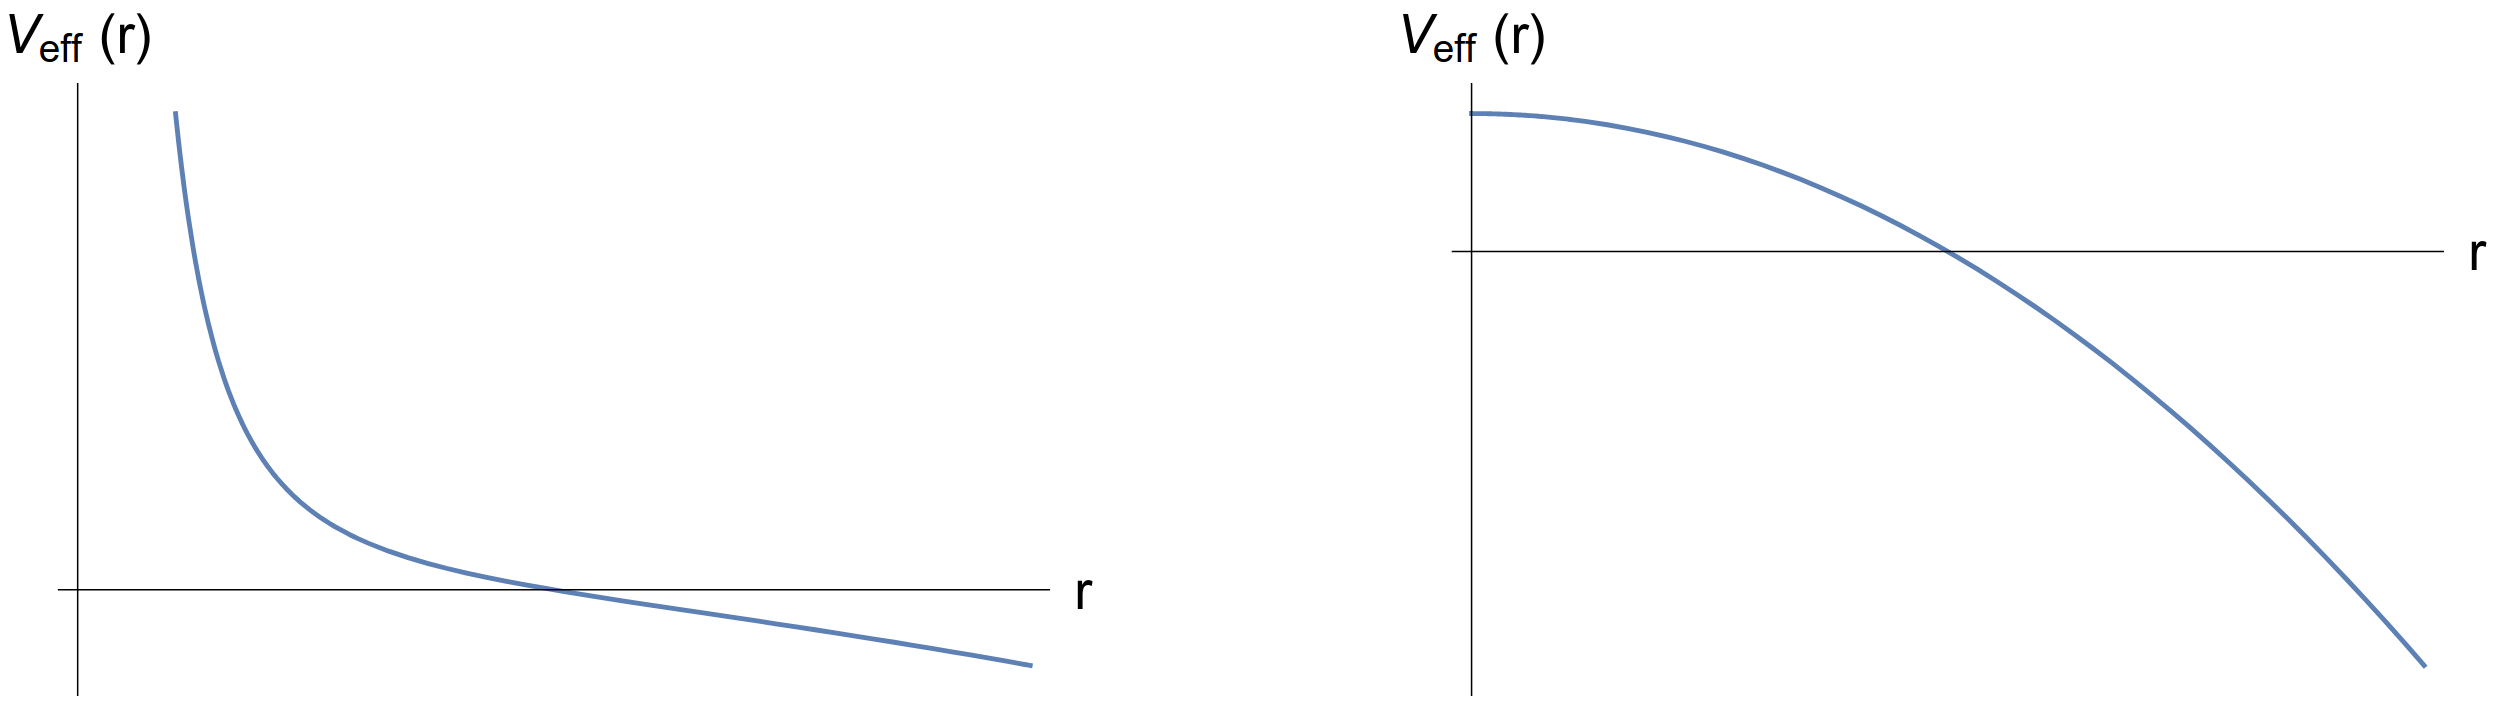
\includegraphics[width = 0.80 \textwidth]{geod-ds.png}
  \caption{Effective potential for de Sitter geodesics, with $ \ell \neq 0 $ and $ \ell = 0 $ respectively.}
  \label{geo-ds}
\end{figure}

For de Sitter space:
\begin{equation*}
  V_{\text{eff}}(r) = \left( 1 + \frac{\ell^2}{r^2} \right) \left( 1 - \frac{r^2}{R^2} \right)
\end{equation*}
This effective potential is plotted in Fig. \ref{geo-ds}: immediately, on sees that the potential pushes the particle to larger values of $ r $. Focusing on geodesics with $ \ell = 0 $, the potential is a harmonic repulsor: a particle stationary at $ r = 0 $ is an unstable geodesic, for if it has non-zero initial velocity it will follow the trajectory:
\begin{equation}
  r(\sigma) = R \sqrt{E^2 - 1} \sinh \frac{\sigma}{R}
  \label{eq:4.19}
\end{equation}
Note that the metric is singular at $ r = R $, a fact not manifest in the geodesic Eq. \ref{eq:4.19} which shows that any observer reaches $ r = R $ in finite proper time. Problems arise when studying the coordinate time $ t $, which has the interpretation of the time experienced by someone stationary at $ r = 0 $; from Eq. \ref{eq:4.16}:
\begin{equation*}
  \frac{dt}{d\sigma} = E \left( 1 - \frac{r^2}{R^2} \right)^{-1}
\end{equation*}
This shows that $ t(\sigma) \rightarrow \infty $ as $ r(\sigma) \rightarrow R $: in fact, if $ r(\sigma^*) = R $, then for $ \sigma = \sigma^* - \varepsilon $ one has $ \frac{dt}{d\sigma} = - \frac{\alpha}{\varepsilon} $, i.e. $ t(\varepsilon) = - \log (\varepsilon / R) $, so $ t(\varepsilon) \rightarrow \infty $ as $ \varepsilon \rightarrow 0 $. This means that a particle moving along the geodesic Eq. \ref{eq:4.19} will reach $ r = R $ in finite proper time, but a stationary observer at $ r = 0 $ will measure an infinite amount of time.\\
This strange behaviour is similar to what happens at the horizon of a black hole ($ r = 2GM $): however, the Schwarzschild metric has a singularity at $ r = 0 $, while de Sitter metric looks flat at $ r = 0 $. de Sitter space seems like an inverted black hole in which particles are pushed outwars to $ r = R $.

\subsubsection{de Sitter embeddings}

de Sitter space can be nicely embedded as a submanifold of $ \R^{1,4} $ with metric:
\begin{equation}
  ds^2 = - (dX^0)^2 + \sum_{i = 1}^{4} (dX^i)^2
  \label{eq:4.20}
\end{equation}
In particular, de Sitter metric Eq. \ref{eq:4.14} is a metric on the submanifold of $ \R^{1,4} $ defined by the timelike hyperboloid:
\begin{equation}
  -(X^0)^2 + \sum_{i = 1}^{4} (X^i)^2 = R^2
  \label{eq:4.21}
\end{equation}
A way of parametrizing this constraint is by imposing that $ r^2 = (X^1)^2 + (X^2)^2 + (X^3)^2 $, so that:
\begin{equation*}
  R^2 - r^2 = (X^4)^2 - (X^0)^2
\end{equation*}
The solutions are parametrized as:
\begin{equation*}
  X^0 = \sqrt{R^2 - r^2} \sinh \frac{t}{R}
  \qquad
  X^4 = \sqrt{R^2 - r^2} \cosh \frac{t}{R}
\end{equation*}
Computing the respective variations, along with $ \sum_{i = 1}^{3} (dX^i)^2 = dr^2 + r^2 d\Omega_2^2 $, where $ d\Omega_n^2 $ is the metric element on $ \mathbb{S}^n $, allows to show that the pull-back of the Minkowski metric Eq. \ref{eq:4.20} on the hyperboloid Eq. \ref{eq:4.21} so parametrized gives the de Sitter metric Eq. \ref{eq:4.14} in the static patch coordinates.\\
The coordinates $ \{X^i\}_{i = 0,\dots,4} $ so defined are not the most intuitive: they single out $ X^4 $ as special, when the constraint does no such thing, and they do not cover the whole hyperboloid, as they are limited to $ X^4 \ge 0 $. A better choice of parametrization is:
\begin{equation*}
  X^0 = R \sinh \frac{\tau}{T}
  \qquad \qquad
  X^i = y^i R \cosh \frac{\tau}{R}
  \,:\,
  \sum_{i = 1}^{4} (y^i)^2 = 1
\end{equation*}
Given this constraint, $ \{y^i\}_{i = 1,,2,3,4} $ parametrize $ \mathbb{S}^3 $. These coordinates retain more of the symmetry of de Sitter space and cover the whole space, thus are a better parametrization. The pull-back of Minkowski metric, however, gives a rather different metric on de Sitter space:
\begin{equation}
  ds^2 = - d\tau^2 + R^2 \cosh^2 \frac{\tau}{R}\, d\Omega_3^2
  \label{eq:4.22}
\end{equation}
These are known as \textit{global coordinates}, as they cover the whole space (except for singularities at the poles for any choice of coordinates on $ \mathbb{S}^3 $). Since this metric is related to that in Eq. \ref{eq:4.14} by a change of coordinates, it too must obey the Einstein equations. Global coordiantes also show that the singularity which happens at $ X^4 $, i.e. at $ r = R $, is nothing but a coordinate singularity.

\begin{figure}
  \centering
  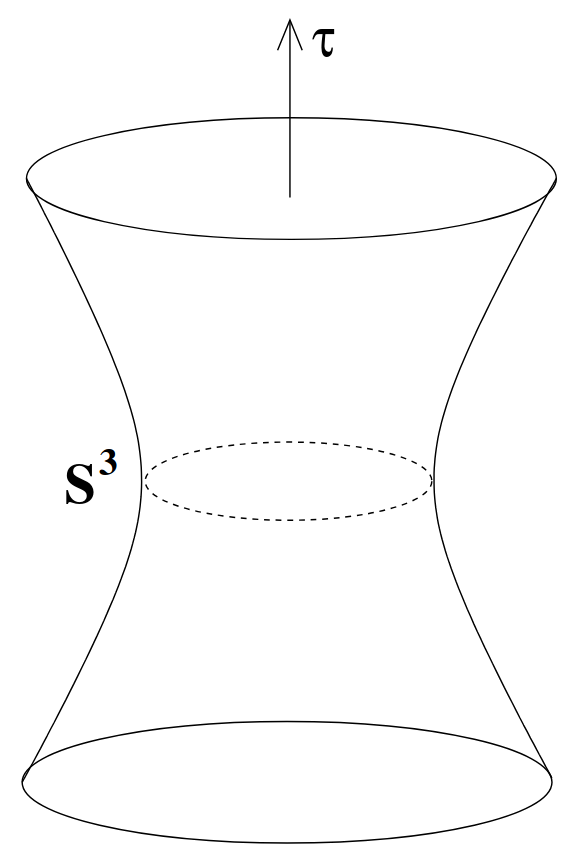
\includegraphics[width = 0.30 \textwidth]{ds-space.png}
  \caption{de Sitter space visualization with global coordinates.}
  \label{ds-space}
\end{figure}

These coordinates provide a clearer intuition for the physics of de Sitter space: it is a time-dependent solution of the field equations in which a spatial $ \mathbb{S}^3 $ first shrinks to a minimal radius $ R $ and then expands, as shown in Fig. \ref{ds-space}. The expansionary phase is a good approximation to our current universe on large scales.

\subsection{Anti-de Sitter space}

Consider $ \Lambda < 0 $. With the same ansatz as for de Sitter space, it's easy to find the metric for \textit{anti-de Sitter space} (AdS):
\begin{equation}
  ds^2 = - \left( 1 + \frac{r^2}{R^2} \right) dt^2 + \left( 1 + \frac{r^2}{R^2} \right)^{-1} dr^2 + r^2 d\Omega_2^2
  \qquad
  R^2 \equiv - \frac{3}{\Lambda}
  \label{eq:4.23}
\end{equation}
Equivalent coordinates are found setting $ r = R \sinh \rho $:
\begin{equation}
  ds^2 = - \cosh^2 \rho\, dt^2 + R^2 d\rho^2 + R^2 \sinh^2 \rho\, d\Omega_2^2
  \label{eq:4.24}
\end{equation}
In AdS there's no coordinate singularity in $ r $ and indeed now coordinates cover the whole space.

\subsubsection{Anti-de Sitter geodesics}

AdS has the same action as in Eq. \ref{eq:4.15}, thus the radial trajectory of a massive particle moving along a geodesic in the $ \vartheta = \frac{\pi}{2} $ plane is $ \dot{r}^2 + V_{\text{eff}}(r) = E^2 $, with:
\begin{equation}
  V_{\text{eff}}(r) = \left( 1 + \frac{\ell^2}{R^2} \right) \left( 1 + \frac{r^2}{R^2} \right)
  \label{eq:4.25}
\end{equation}

\begin{figure}
  \centering
  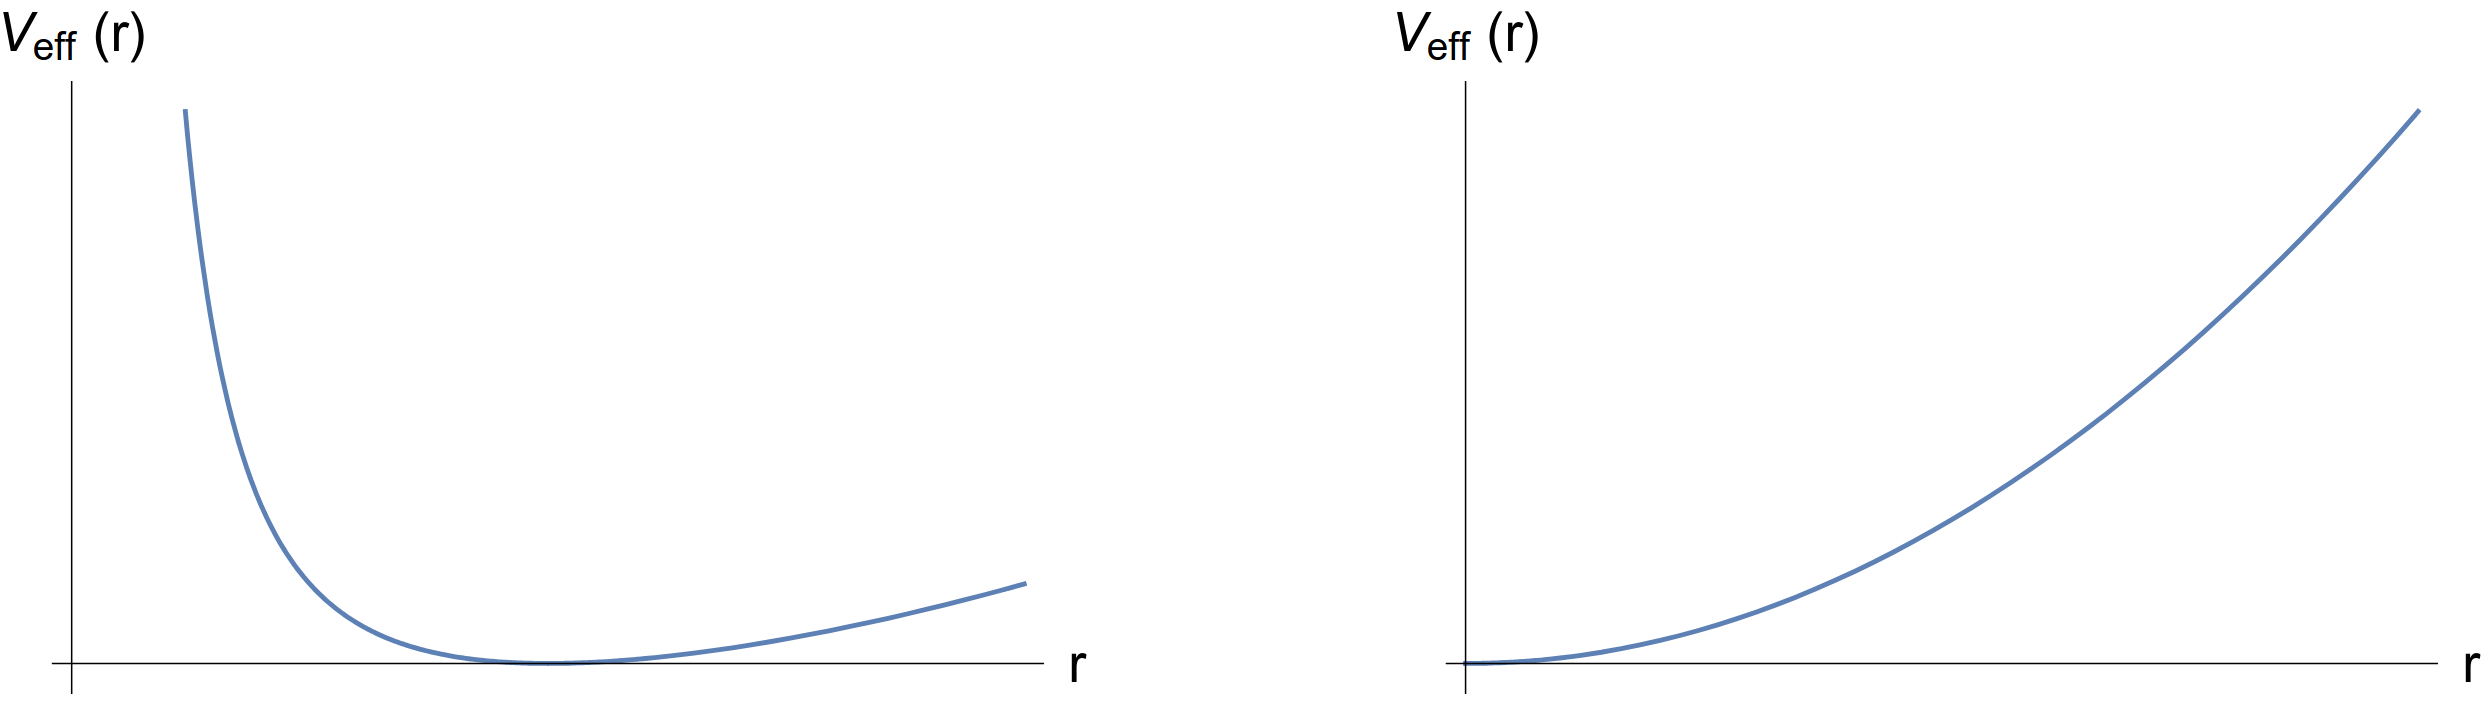
\includegraphics[width = 0.80 \textwidth]{geod-ads.png}
  \caption{Effective potential for anti-de Sitter geodesics, with $ \ell \neq 0 $ and $ \ell = 0 $ respectively.}
  \label{geo-ads}
\end{figure}

Plotting it in Fig. \ref{geo-ads}, the geodesics' behavior is clear: with no angular momentum, anti-de Sitter space acts like a harmonic oscillator, pulling the particle towards the origin and making it oscillate around $ r = 0 $. If the particle has non-zero angular momentum, then the potential has a minimum at $ r_*^2 = R \ell $, thus particles oscillate around $ r_* $: importantly, particles with finite energy cannot escape to $ r \rightarrow \infty $, but are constrained by the spacetime within some finite distance from the origin.\\
This picture of AdS as a harmonic trap which pulls particle to the origin clashes with the fact that AdS is a homogeneous space (roughly, all points are the same). To understand how these two facts are compatible, consider a stationary observer at $ r = 0 $: this is a geodesic and, from its perspective, other observers (with $ \ell = 0 $) will oscillate around $ r = 0 $ along geodesics. However, since these observers move along geodesics, in their reference frame they are stationary at $ r = 0 $, with all other observers oscillating. Thus, while in dS each observer views themselves at the center of the universe, with other observers moving away from them, in AdS each observer views themselves as the center of the universe, with other observer oscillating around them.\\
Its possible to study geodesics for a massless particle too. This time, the constraint to the action is:
\begin{equation*}
  - f(r)^2 \dot{t}^2 + f(r)^{-2} \dot{r}^2 + r^2 (\dot{\vartheta}^2 + \sin^2 \vartheta \dot{\varphi}^2) = 0
\end{equation*}
This means that the particle follows a null geodesic. Its equation of motion is:
\begin{equation*}
  \dot{r}^2 + V_{\text{null}}(r) = E^2
  \qquad
  V_{\text{null}}(r) = \frac{\ell^2}{r^2} \left( 1 + \frac{r^2}{R^2} \right)
\end{equation*}

\begin{figure}
  \centering
  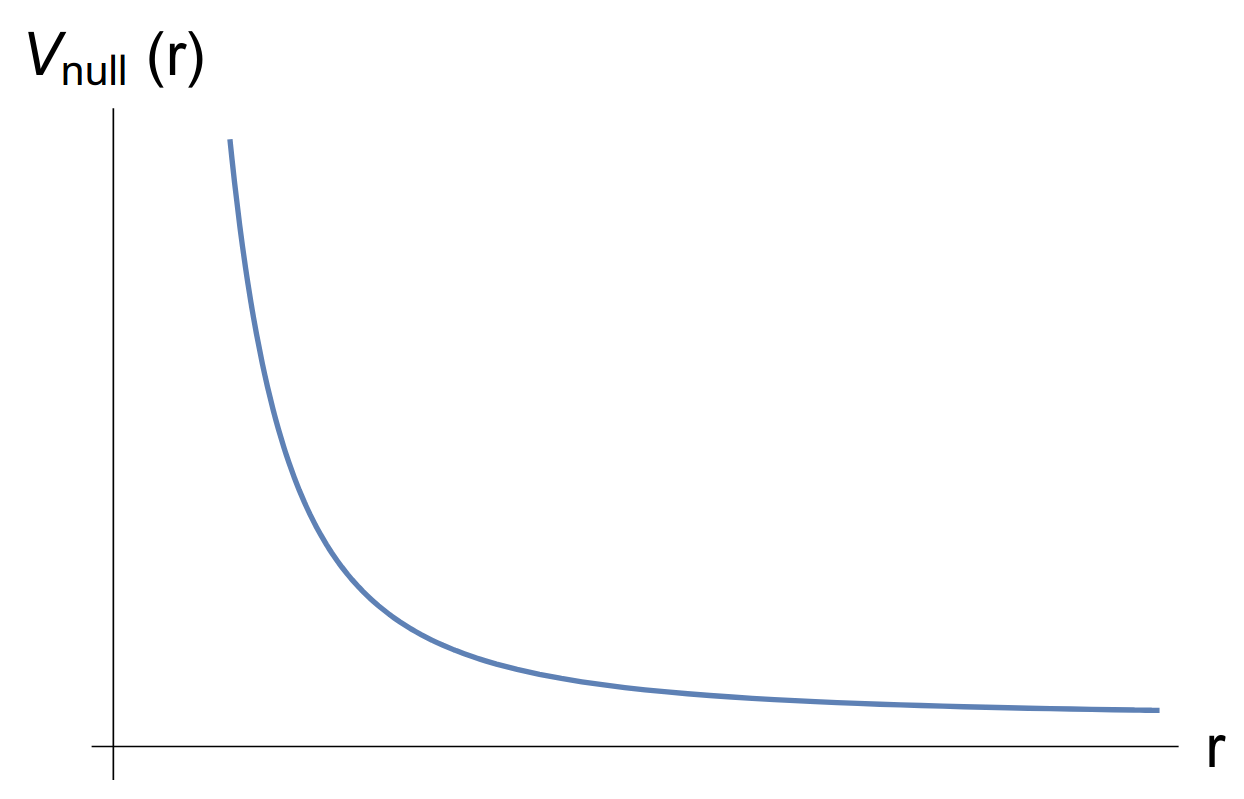
\includegraphics[width = 0.50 \textwidth]{ads-pot.png}
  \caption{Potential experienced by massless particles with $ \ell \neq 0 $ in AdS.}
  \label{ads-pot}
\end{figure}

Its plot in Fig. \ref{ads-pot} makes it clear that massless particle can escape to $ r \rightarrow \infty $, as the null potential is asymptotically constant, and it will only experience the usual gravitational redshift. AdS only confines massive particles.
To solve for the trajectory, it's easier to work with $ r = R \sinh \rho $ and $ \ell = 0 $, so that:
\begin{equation*}
  R \dot{\rho} = \pm \frac{E}{\cosh \rho}
  \quad \Rightarrow \quad
  R \sinh \rho(\sigma) = E (\sigma - \sigma_0)
\end{equation*}
One sees that $ \rho \rightarrow \infty $ only in infinite affine time (i.e. $ \sigma \rightarrow \infty $). However, in coordinate time, recalling Eq. \ref{eq:4.16}, $ E = \cosh^2 \rho\, \dot{t} $, so:
\begin{equation*}
  R \tan \frac{t}{R} = E (\sigma - \sigma_0)
\end{equation*}
Hence, as affine time $ \sigma \rightarrow \infty $, coordinate time $ t \rightarrow \frac{\pi}{2} R $. This means that light rays escape to infinity in a finite amount of coordinate time: to make sense of dynamics in AdS, one must specify some boundary conditions at infinity to dictate how massless particles and field behave.\\
AdS does not appear to be of any cosmological interest.

\subsubsection{Anti-de Sitter embeddings}

AdS too has a natural embedding in a 5d spacetime: it is a submanifold of $ \R^{2,3} $ with metric:
\begin{equation}
  ds^2 = - (dX^0)^2 - (dx^4)^2 + \sum_{i = 1}^{3} (dX^i)^2
  \label{eq:4.26}
\end{equation}
In particular, anti-de Sitter metric Eq. \ref{eq:4.23} is a metric on the hyperboloid:
\begin{equation}
  - (X^0)^2 - (X^4)^2 + \sum_{i = 1}^{3} (X^i)^2 = - R^2
  \label{eq:4.27}
\end{equation}
This constraint can be solved via the parametrization:
\begin{equation*}
  X^0 = R \cosh \rho \sin \frac{t}{R}
  \qquad
  X^4 = R \cosh \rho \cos \frac{t}{R}
  \qquad
  X^i = y^i R \sinh \rho
  \,:\,
  \sum_{i = 1}^{3} (y^i)^2 = 1
\end{equation*}
Given this constraint, $ \{y^i\}_{i = 1,2,3} $ parametrize $ \mathbb{S}^2 $. The pull-back of the metric Eq. \ref{eq:4.26} on the hyperboloid so parametrized gives anti-de Sitter metric Eq. \ref{eq:4.24}.\\
There's a small subtlety: the embedding hyperboloid has topology $ \mathbb{S}^1 \times \R^3 $, not $ \R^4 $: this corresponds to a compact time direction, as $ t \in [0, 2\pi R) $. However, AdS metric does not have such restriction, with $ t \in \R $: this is a universal covering of the hyperboloid.\\
Another useful parametrization of the hyperboloid is the following:
\begin{equation*}
  X^4 - X^3 = r
  \qquad
  X^4 + X^3 = \frac{R^2}{r} + \frac{r}{R^2} \eta_{ij} dx^i dx^j
  \qquad
  X^i = \frac{r}{R} x^i
  \,,\, i = 0,1,2
\end{equation*}
with $ r \in [0, \infty) $. With these coordinates, the metric takes the form:
\begin{equation*}
  ds^2 = R^2 \frac{dr^2}{r^2} + \frac{r^2}{R^2} \eta_{ij} dx^i dx^j
\end{equation*}
These coordinates don't cover the whole AdS, but only one-half of the hyperboloid, restricted to $ X^4 - X^3 > 0 $: this is known as the \textit{Poincaré patch} of AdS. Moreover, $ x^0 $ cannot be further extended beyond $ x^0 \in (-\infty, +\infty) $, thus in global coordinates the restriction $ t \in [0,2\pi R) $ remains. In this case, massive particles fall towards $ r = 0 $.\\
Finally, there are two more possible coordinate systems on the Poincaré patch, obtained by setting $ z = \frac{R^2}{r} $ and $ r = R e^\rho $:
\begin{equation*}
  ds^2 = \frac{R^2}{z^2} \left( dz^2 + \eta_{ij} dx^i dx^j \right)
  \qquad \qquad
  ds^2 = R^2 d\rho^2 + e^{2\rho} \eta_{ij} dx^i dx^j
\end{equation*}
In each case, massive particles fall towards $ z = \infty $ or $ \rho = -\infty $.

\section{Symmetries}

What makes Minkowski, dS and AdS special solutions to the Einstein equations are their symmetries.\\
The symmetries of Minkowski spacetime are familiar: translations and rotations of spacetime, with the latter splitting between proper rotations and Lorentz boosts. These symmetries are responsible for the existence of energy, momentum and angular momentum on a fixed Minkowski background.\\
It is important to characterize the symmetries of a general metric.

\subsection{Isometries}

Recall Def. \ref{def-flow} of flow on a manifold: by Eq. \ref{eq:2.10}, it is possible to identify a flow with a vector field $ K \in \xm $ such that it is tangent to the flow at each point of the manifold: $ K^\mu = \frac{dx^\mu}{dt} $, with $ x^\mu(t) \equiv x^\mu(\sigma_t) $.

\begin{definition}
  Given a flow associated to $ K \in \xm $, it is said to be an \textit{isometry} if:
  \begin{equation}
    \ld_K g = 0
    \quad \Leftrightarrow \quad
    \na_\mu K_\nu + \na_\nu K_\mu = 0
    \label{eq:4.28}
  \end{equation}
\end{definition}
Recall Eqq. \ref{eq:4.11}-\ref{eq:4.12} for the equivalence. This condition means that the metric doesn't change along flow lines: this is called \textit{Killing equation}, and a vector field which satisfied it is a \textit{Killing vector field}.
Prop. \ref{prop-lie-algebra} can be generalized to hold for the Lie derivative of arbitrary tensor fields, thus Killing vectors too form a Lie algebra: it is the Lie algebra of the isometry group of the manifold.

\begin{example}
  Given a metric $ g_{\mu \nu}(x) $, if it doesn't depend on $ x^1 \equiv y $, then $ X = \pa_y $ is a Killing vector field, for $ (\ld_{\pa_y} g)_{\mu \nu} = \pa_y g_{\mu \nu} = 0 $. This is the case of ignorable degrees of freedom, as in Eqq. \ref{eq:4.16}-\ref{eq:4.17}.
\end{example}

\subsubsection{Minkowski spacetime}

Consider Minkowski spacetime $ \R^{1,3} $ with $ g_{\mu \nu} = \eta_{\mu \nu} $. Killing equation is:
\begin{equation*}
  \pa_\mu K_\nu + \pa_\nu K_\mu = 0
\end{equation*}
There two forms of solution. The first one is:
\begin{equation*}
  K_\mu = c_\mu
\end{equation*}
for any constant vector $ c_\mu $. These generate translations. Alternatively:
\begin{equation*}
  K_\mu = \omega_{\mu \nu} x^\nu
  \,:\, \omega_{\mu \nu} = - \omega_{\nu \mu}
\end{equation*}
These generate rotations and Lorentz boosts. The emergence of the Lie algebra structure can be elucidated defining the Killing vectors:
\begin{equation*}
  P_\mu \defeq \pa_\mu
  \qquad
  M_{\mu \nu} \defeq \eta_{\mu \rho} x^\rho \pa_\nu - \eta_{\nu \rho} x^\rho \pa_\mu
\end{equation*}
These are 10 Killing vectors: 4 for translations and 6 for rotations and boosts.

\begin{proposition}
  Killing vectors of Minkowski spacetime obbey:
  \begin{equation*}
    [P_\mu, P_\nu] = 0
    \qquad
    [M_{\mu \nu}, P_\sigma] = - \eta_{\mu \sigma} P_\nu + \eta_{\sigma \nu} P_\mu
  \end{equation*}
  \begin{equation*}
    [M_{\mu \nu}, M_{\rho \sigma}] = \eta_{\mu \sigma} M_{\nu \rho} + \eta_{\nu \rho} M_{\mu \sigma} - \eta_{\mu \rho} M_{\nu \sigma} - \eta_{\nu \sigma} M_{\mu \rho}
  \end{equation*}
\end{proposition}
\begin{proof}
  By direct calculation.
\end{proof}

This is precisely the Lie algebra of the Poincaré group $ \R^4 \times \SOn{1,3} $, i.e. the isometry group of Minkowski spacetime.

\subsubsection{de Sitter and anti-de Sitter space}

The isometries of dS and AdS are best seen from their embeddings.
The constraint Eq. \ref{eq:4.21} which defined de Sitter space is invariant under the rotations of $ \R^{1,4} $, thus dS inherits the $ \SOn{1,4} $ isometry group. Similarly, the constraint Eq. \ref{eq:4.27} which defines anti-de Sitter space is invariant under rotations of $ \R^{2,3} $, so AdS inherits the $ \SOn{2,3} $ isometry group. Note that both these groups are 10-dimensional, as $ \R^4 \times \SOn{1,3} $.\\
It's simple to determine the 10 Killing spinors of 5d spacetime:
\begin{equation*}
  M_{AB} = \eta_{AC} X^C \pa_B - \eta_{BC} X^C \pa_A
\end{equation*}
where $ X^A, A = 0,1,2,3,4 $ are 5d coordinates and $ \eta_{AB} $ is the appropriate Minkowski metric, with signature $ (-,+,+,+,+) $ for dS and $ (-,-,+,+,+) $ for AdS. In either case, the Lie algebra is that of the appropriate Lorentz group:
\begin{equation*}
  [M_{AB}, M_{CD}] = \eta_{AD} M_{BC} + \eta_{BC} M_{AD} - \eta_{AC} M_{BD} - \eta_{BD} M_{AC}
\end{equation*}
The embedding hyperbolae are both invariant under these Killing vectors: flows generated by them map points on the hyperbolae to other points on the hyperbolae. Therefore, these Killing vectors are inherited by dS and AdS respectively.

\paragraph{Energy}

Energy is defined by timelike Killing vectors. In anti-de Sitter space there's no problem finding a timelike Killing vector, as the metric in global coordinates Eq. \ref{eq:4.24} is time-independent, so $ K = \pa_t $. However, this changes in de Sitter space.\\
Considering dS in the static patch with coordinates $ r^2 = (X^1)^2 + (X^2)^2 + (X^3)^2 $, $ X^0 = \sqrt{R^2 - r^2} \sinh \frac{t}{R} $ and $ X^4 = \sqrt{R^2 - r^2} \cosh \frac{t}{R} $, the metric Eq. \ref{eq:4.14} is time-independent, thus $ K = \pa_t $ is a Killing vector; pushing it forward to the 5d space:
\begin{equation*}
  \pa_t = \frac{\pa X^A}{\pa t} \pa_A = \frac{1}{R} ( X^4 \pa_0 + X^0 \pa_4 )
\end{equation*}
On the static patch, this Killing vector is timelike and the energy Eq. \ref{eq:4.16} follows from it. The problem is that the static patch is only one-half of the hyperboloid: when considering the whole AdS, one must account for the case $ X^0 = 0, X^4 < 0 $, in which the Killing vector points in the past direction, or $ X^0 \neq 0, X^4 = 0 $, in which it is spacelike. Therefore, the Killing vector can be both timelike (future-directed and past-directed) or spacelike when spanning the whole manifold: for this reason, it's not possible to define a global positive conserved energy on the total de Sitter space. The same conclusion follows by noting that the metric in global coordinates Eq. \ref{eq:4.22} is time-dependent.

\subsection{Conserved quantities}

It is possible to reframe Noether's theorem in the context of Killing vectors.

\begin{theorem}[Noether]
  Given a massive particle moving on a geodesic $ x^\mu(\tau) $ in a spacetime with metric $ g $ which admits a Killing vector field $ K $, then the \textit{Noether charge} is conserved along the geodesic:
  \begin{equation}
    Q \defeq K_\mu \frac{dx^\mu}{d\tau}
    \label{eq:4.29}
  \end{equation}
\end{theorem}
\begin{proof}
  First, show that $ Q $ is indeed conserved along the geodesic, recalling Eq. \ref{eq:4.28}:
  \begin{equation*}
    \frac{dQ}{d\tau} = \pa_\nu K_\mu \frac{dx^\nu}{d\tau} \frac{dx^\mu}{d\tau} + K_\mu \frac{d^2 x^\mu}{d\tau^2} = \pa_\nu K_\mu \frac{dx^\nu}{d\tau} - K_\mu \Gamma^\mu_{\rho \sigma} \frac{dx^\rho}{d\tau} \frac{dx^\sigma}{d\tau} = \na_\nu K_\mu \frac{dx^\nu}{d\tau} \frac{dx^\mu}{d\tau} = 0
  \end{equation*}
  To show that $ Q $ follows from Noether's theorem, consider the action of the massive particle and introduce an infinitesimal transformation $ \delta x^\mu = K^\mu (x) $:
  \begin{equation*}
    \begin{split}
      \delta \mathcal{S}
      &= \delta \int d\tau\, g_{\mu \nu}(x) \frac{dx^\mu}{d\tau} \frac{dx^\nu}{d\tau} = \int d\tau \left[ \pa_\rho g_{\mu \nu} \frac{dx^\mu}{d\tau} \frac{dx^\nu}{d\tau} \delta x^\rho + 2 g_{\mu \nu} \frac{dx^\mu}{d\tau} \frac{d \delta x^\nu}{d\tau} \right] \\
      &= \int d\tau \left[ \pa_\rho g_{\mu \nu} \frac{dx^\mu}{d\tau} \frac{dx^\nu}{d\tau} K^\rho + 2 \frac{dx^\mu}{d\tau} \left( \frac{dK_\mu}{d\tau} - K^\nu \frac{dg_{\mu \nu}}{d\tau} \right) \right] \\
      &= \int d\tau \left[ \pa_\rho g_{\mu \nu} K^\rho - 2 K^\rho \pa_\nu g_{\mu \rho} + 2 \pa_\nu K_\mu \right] \frac{dx^\mu}{d\tau} \frac{dx^\nu}{d\tau} = \int d\tau\, 2 \na_\nu K_\mu \frac{dx^\mu}{d\tau} \frac{dx^\nu}{d\tau}
    \end{split}
  \end{equation*}
  The transformation is a symmetry if $ \delta \mathcal{S} = 0 $, thus, by the symmetry of $ \frac{dx^\mu}{d\tau} \frac{dx^\nu}{d\tau} $, the resulting equation is $ \na_{(\nu} K_{\mu)} = 0 $, i.e. Killing equation.
\end{proof}

\begin{example}
  Energy and angular momentum defined on de Sitter geodesics by Eqq. \ref{eq:4.16}-\ref{eq:4.17} are Noether charges associated to Killing vectors $ \pa_t $ and $ \pa_\varphi $ respectively.
\end{example}

\subsection{Komar integrals}

\begin{definition}
  Given a Killing vector $ K = K^\mu \pa_\mu $, defined the 1-form $ K \equiv K_\mu dx^\mu $, the associated \textit{Komar form} is the 2-form defined as:
  \begin{equation}
    F \defeq dK
    \label{eq:4.30}
  \end{equation}
\end{definition}

\begin{proposition}
  Given a Killing vector $ K = K^\mu \pa_\mu $, the associated Komar form is:
  \begin{equation}
    F_{\mu \nu} = \na_\mu K_\nu - \na_\nu K_\mu
    \label{eq:4.31}
  \end{equation}
\end{proposition}
\begin{proof}
  $ F = \frac{1}{2} F_{\mu \nu} dx^\mu \wedge dx^\nu = dK = \na_\mu K_\nu dx^\mu \wedge dx^\nu $.
\end{proof}

\begin{theorem}
  If the vacuum Einstein equations $ R_{\mu \nu} = 0 $ hold, then a Komar form obeys the vacuum Maxwell equations:
  \begin{equation}
    d \star F = 0
    \quad \Leftrightarrow \quad
    \na^\mu F_{\mu \nu} = 0
    \label{eq:4.32}
  \end{equation}
\end{theorem}
\begin{proof}
  Recall Prop. \ref{prop-max-eq} for the equivalence. From Ricci identity Eq. \ref{eq:3.38}:
  \begin{equation*}
    (\na_\mu \nu_\nu - \na_\nu \na_\mu) K^\sigma = \tensor{R}{^\sigma_{\rho \mu \nu}} K^\rho
    \quad \Rightarrow \quad
    (\na_\mu \na_\nu - \na_\nu \na_\mu) K^\mu = R_{\rho \nu} K^\rho
  \end{equation*}
  From Killing equation $ \na_{(\mu} K_{\nu)} = 0 \,\Rightarrow\, \na_\mu K^\mu = 0 $, thus $ \na_\mu \na_\nu K^\mu = R_{\rho \nu} K^\rho $ and:
  \begin{equation*}
    \na^\mu F_{\mu \nu} = \na^\mu \na_\mu K_\nu - \na^\mu \na_\nu K_\mu = -2 \na^\mu \na_\nu K_\mu = -2 R_{\rho \nu} K^\rho
  \end{equation*}
  If $ R_{\rho \nu} = 0 $, then $ \na^\mu F_{\mu \nu} = 0 $.
\end{proof}

\begin{definition}
  Given a Komar form $ F $ associated to a Killing vector $ K $, the associated \textit{Komar charge} (or Komar integral) on a spatial submanifold $ \Sigma $ is defined as:
  \begin{equation}
    Q_{\text{Komar}} \defeq - \frac{1}{8\pi G} \int_\Sigma d \star F = - \frac{1}{8\pi G} \int_{\pa \Sigma} \star\, F = - \frac{1}{8\pi G} \int_{\pa \Sigma} \star\, dK
    \label{eq:4.33}
  \end{equation}
\end{definition}

\begin{proposition}
  If Eq. \ref{eq:4.32} holds, then $ Q_{\text{Komar}} $ is conserved.
\end{proposition}
\begin{proof}
  Recall Eq. \ref{eq:3.49}: the proof is identical.
\end{proof}

As for Noether integrals of a particle, Komar integrals of spacetime are interpreted based on the defining Killing vector. For example, if $ K^\mu $ is everywhere timelike, i.e. $ g_{\mu \nu} K^\mu K^\nu < 0 $, then its Komar integral can be identified with the energy (or the mass) of spacetime; if the Killing vector is related to rotations, instead, the conserved charge is the angular momentum of spacetime.

\section{Asymptotics of spacetime}

The three special solution (Minkowski, dS, AdS) not only have different spacetime curvature and symmetries, but, more fundamentally, they have different behavior at infinity. Their importance lie in the fact that, however complicated the metric might be, if fields are suitably localized, then they will asymptote to one of these three symmetric spaces.

\subsection{Conformal transformations}

\begin{definition}
  Given a metric manifold $ (\mathcal{M},g) $ and a non-vanishing $ \Omega \in \cm $, a \textit{conformal transformation} is defined as:
  \begin{equation}
    \tilde{g}_{\mu \nu}(x) = \Omega^2(x) g_{\mu \nu}(x)
    \label{eq:4.34}
  \end{equation}
\end{definition}

Typically, $ g $ and $ \tilde{g} $ describe different spacetime with considerably warped distances. However, conformal transformations preserve angles: in Lorentzian spacetime, the two metrics have the same causal structure, i.e. null/timelike/spacelike vector fields in one metric remain null/timelike/spacelike in the other too.

\begin{proposition}
  Only conformal transformations of the metric preserve its causal structure.
\end{proposition}

Although timelike particle trajectories necessarily remain timelike under a conformal transformation, the same needs not be true for geodesics, as distances get warped.

\begin{proposition}
  Null geodesics are mapped to null geodesics under a conformal transformation.
\end{proposition}
\begin{proof}
  First compute the Christoffel symbols in the new metric:
  \begin{equation*}
    \begin{split}
      \Gamma^\mu_{\rho \sigma}[\tilde{g}]
      &= \frac{1}{2} \tilde{g}^{\mu \nu} (\pa_\rho \tilde{g}_{\nu \sigma} + \pa_\sigma \tilde{g}_{\rho \nu} - \pa_\nu \tilde{g}_{\rho \sigma}) \\
      &= \frac{1}{2} \Omega^{-2} g^{\mu \nu} (\pa_\rho (\Omega^2 g_{\nu \sigma}) + \pa_\sigma (\Omega^2 g_{\rho \nu}) - \pa_\nu (\Omega^2 g_{\rho \sigma})) \\
      &= \Gamma^\mu_{\rho \sigma}[g] + \Omega^{-1} (\delta^\mu_\sigma \na_\rho \Omega + \delta^\mu_\rho \na_\sigma \Omega - g_{\rho \sigma} \na^\mu \Omega)
    \end{split}
  \end{equation*}
  In the last line, recall that $ \na = \pa $ on scalar functions. Suppose an affinely parametrized geodesic in the metric $ g $:
  \begin{equation*}
    \frac{d^2 x^\mu}{d\tau^2} + \Gamma^\mu_{\rho \sigma}[g] \frac{dx^\rho}{d\tau} \frac{dx^\sigma}{d\tau} = 0
    \quad \Rightarrow \quad
    \frac{dx^2 x^\mu}{d\tau^2} + \Gamma^\mu_{\rho \sigma}[\tilde{g}] \frac{dx^\rho}{d\tau} \frac{dx^\sigma}{d\tau} = \Omega^{-1} (\delta^\mu_\sigma \na_\rho \Omega + \delta^\mu_\rho \na_\sigma \Omega - g_{\rho \sigma} \na^\nu \Omega) \frac{dx^\rho}{d\tau} \frac{dx^\sigma}{d\tau}
  \end{equation*}
  For a null geodesic $ g_{\rho \sigma} \frac{dx^\rho}{d\tau} \frac{dx^\sigma}{d\tau} = 0 $, thus:
  \begin{equation*}
    \frac{dx^2 x^\mu}{d\tau^2} + \Gamma^\mu_{\rho \sigma}[\tilde{g}] \frac{dx^\rho}{d\tau} \frac{dx^\sigma}{d\tau} = 2 \frac{dx^\mu}{d\tau} \frac{1}{\Omega} \frac{d\Omega}{d\tau}
  \end{equation*}
  This is the equation of non-affinely parametrized geodesic (like Eq. \ref{eq:1.16}), hence the thesis.
\end{proof}

Usual curvature tensors are not invariant under conformal transformations. A curvature tensor that is indeed invariant is the \textit{Weyl tensor}:
\begin{equation}
  C_{\mu \nu \rho \sigma} \defeq R_{\mu \nu \rho \sigma} - \frac{2}{n - 2} \left( g_{\mu [\rho} R_{\sigma] \nu} - g_{\nu [\rho} R_{\sigma] \mu} \right) + \frac{2}{(n-1)(n-2)} R g_{\mu [\rho} g_{\sigma] \nu}
  \label{eq:4.35}
\end{equation}
where $ n \equiv \dim_{\R}\mathcal{M} $. The Weyl tensor has all the symmetries of the Riemann tensor, with the additional property that it vanishes when contracting any pair of indices with the metric: it can be viewed as the trace-free part of the Riemann tensor.

\subsection{Penrose diagrams}

To study the asymptotic behavior of spacetime, one needs to perform a conformal transformation that maps infinity to a finite distance: the resulting causal structure can then be drawn on a finite area and the resulting picture is called a \textit{Penrose diagram}.

\subsubsection{Minkowski spacetime}

It is simplest to study $ \R^{1,1} $, where the Minkowski metric is $ ds^2 = -dt^2 + dx^2 $. First, introduce \textit{lightcone coordinates}:
\begin{equation*}
  u = t - x
  \qquad
  v = t + x
  \quad \Rightarrow \quad
  ds^2 = - du\, dv
\end{equation*}
These coordinates range in $ u,v \in \R $. To work with finite quantities, define:
\begin{equation*}
  u = \tan \tilde{u}
  \qquad
  v = \tan \tilde{v}
  \quad \Rightarrow \quad
  ds^2 = - \frac{1}{\cos^2 \tilde{u}\, \cos^2 \tilde{v}} d\tilde{u}\, d\tilde{v}
\end{equation*}
where now $ \tilde{u},\tilde{v} \in \left( -\frac{\pi}{2}, +\frac{\pi}{2} \right) $. Note that the metric diverges when approaching the boundary of Minkowski spacetime. However, a conformal transformation is possible with $ \Omega(\tilde{u},\tilde{v}) \equiv \cos \tilde{u}\, \cos \tilde{v} $:
\begin{equation*}
  d\tilde{s}^2 = \left( \cos^2 \tilde{u}\, \cos^2 \tilde{v} \right) ds^2 = - d\tilde{u}\, d\tilde{v}
\end{equation*}
It is now possible to add $ \tilde{u} = \pm \frac{\pi}{2} $ and $ \tilde{v} = \pm \frac{\pi}{2} $: this operation is called \textit{conformal compactification}.

\begin{figure}
  \centering
  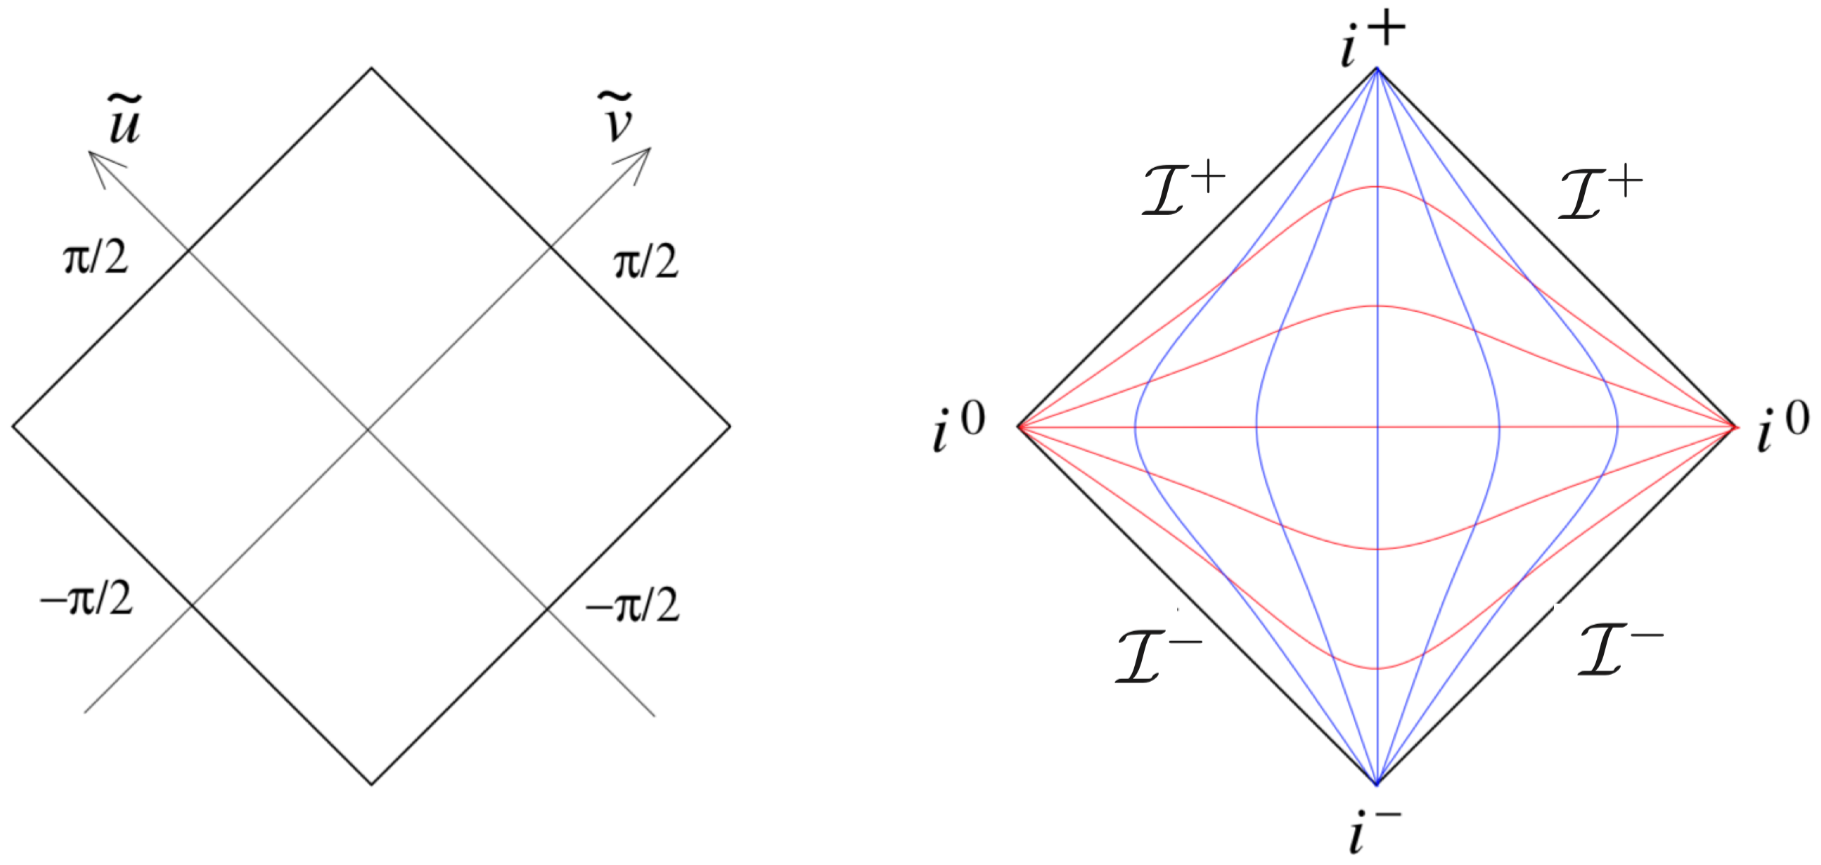
\includegraphics[width = 0.70 \textwidth]{ms-causal.png}
  \caption{Penrose diagram for $ d = 1 + 1 $ Minkowski spacetime.}
  \label{ms-causal}
\end{figure}

Penrose diagrams, as other relativistic diagrams, present light-rays travelling at 45°, time in the vertical direction and space in the horizontal one. Fig. \ref{ms-causal} shows the Penrose diagram for Minkowski spacetime $ \R^{1,1} $ with $ \tilde{u},\tilde{v} $ coordinates, both with coordinate axis and geodesics. Moreover, the various infinities of Minkowski space are shown:
\begin{itemize}
  \item timelike geodesics (blue) start at $ i^- (\tilde{u},\tilde{v}) = \left( -\frac{\pi}{2}, -\frac{\pi}{2} \right) $ and end at $ i^+ (\tilde{u},\tilde{v}) = \left( +\frac{\pi}{2}, +\frac{\pi}{2} \right) $, called respectively \textit{past} and \textit{future timelike infinity};
  \item spacelike geodesics (red) start and end at $ i^0 (\tilde{u},\tilde{v}) = \left( \mp \frac{\pi}{2}, \pm \frac{\pi}{2} \right) $, both called \textit{spacelike infinity};
  \item all null curves (not shown) start at the boundary $ \mathcal{I}^- \equiv \{\tilde{u} = - \frac{\pi}{2}\} \cup \{\tilde{v} = - \frac{\pi}{2}\} $ and end at the boundary $ \mathcal{I}^+ \equiv \{\tilde{u} = +\frac{\pi}{2}\} \cup \{\tilde{v} = +\frac{\pi}{2}\} $, called respectively \textit{past} and \textit{future null infinity}.
\end{itemize}
It's clear that in Minkowski spacetime there are more ways reach infinity along a null direction than in a timelike or spacelike direction.

\begin{figure}
  \centering
  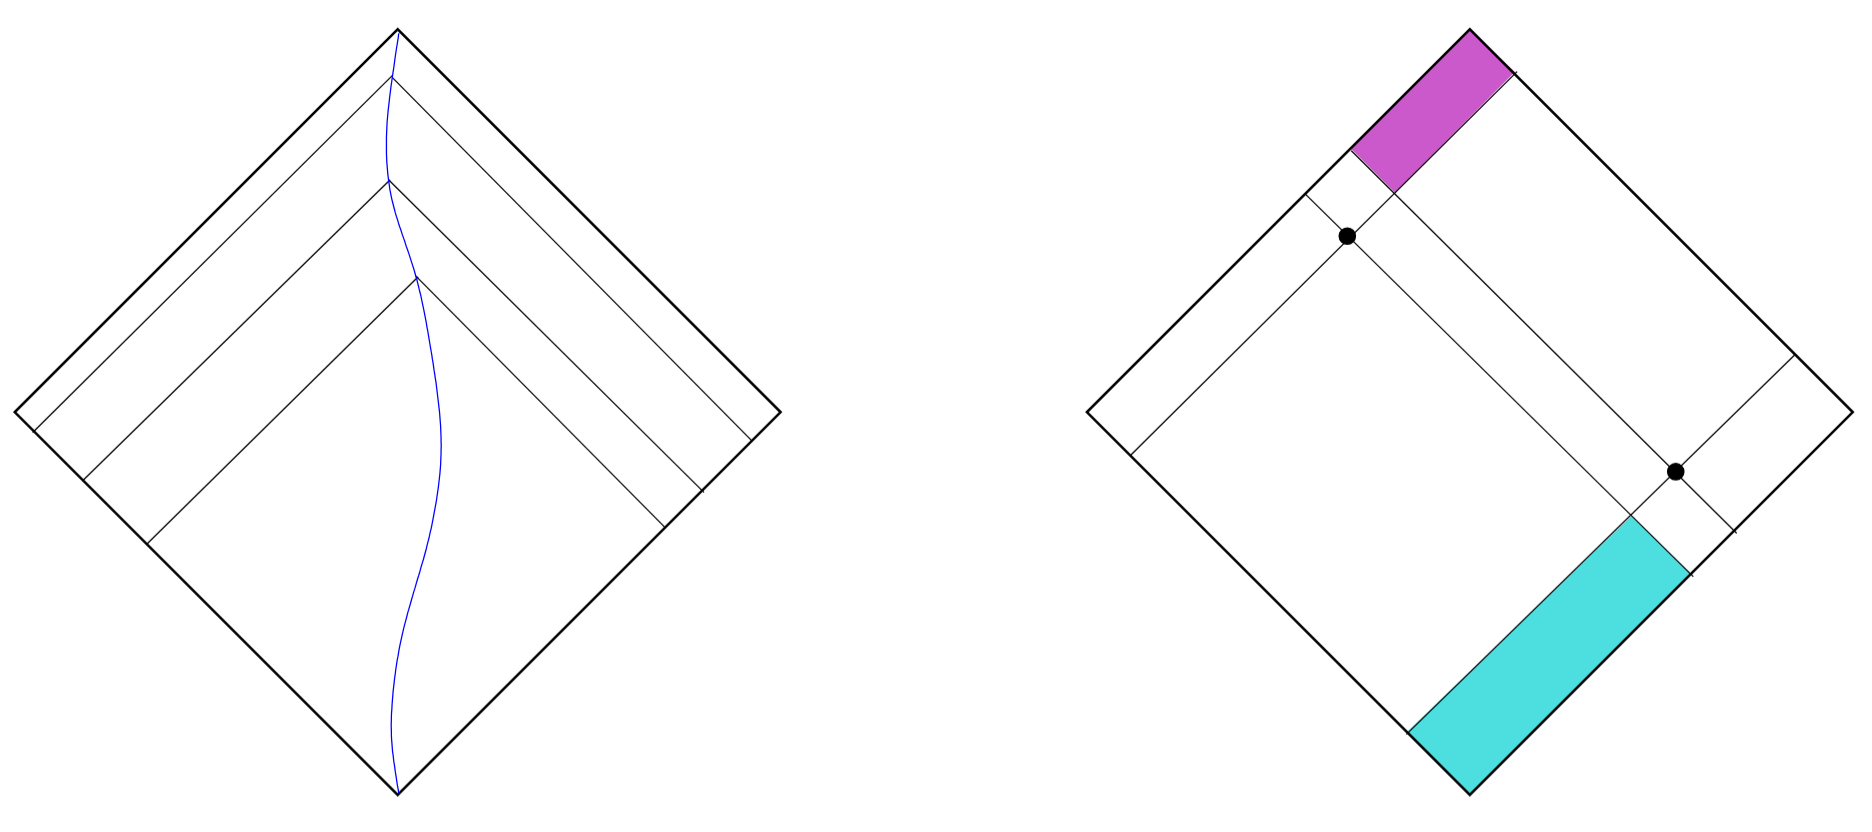
\includegraphics[width = 0.70 \textwidth]{ms-light.png}
  \caption{Lightcones in $ d = 1 + 1 $ Minkowski spacetime.}
  \label{ms-light}
\end{figure}

Penrose diagrams allow to immediately visualize the causal structure of spacetime. As shown in Fig. \ref{ms-light}, given a particle moving along a timelike curve, as it approaches $ i^+ $ its past lightcone encompasses progressively more of spacetime: thus, an observer in Minkowski spacetime can in principle see everything, as long as they wait long enough. Relatedly, given any two points in Minkowski spacetime, they are causally connected both in the past and in the future, as both cones intersect (see Fig. \ref{ms-light}): thus, there was always an event in the past that could have influenced both, and there will always be an event in the future that can be influenced by both.

\paragraph{4d Minkowski spacetime}

The analysis can be repeated for $ \R^{1,3} $ with $ ds^2 = -dt^2 + dr^2 + r^2 d\Omega_2^2 $. Lightcone coordinates are again:
\begin{equation*}
  u = t - r
  \qquad
  v = t + r
  \quad \Rightarrow \quad
  ds^2 = - du\, dv + \frac{1}{4} \left( u - v^2 \right) d\Omega_2^2
\end{equation*}
Finite range coordinates are again:
\begin{equation*}
   u = \tan \tilde{u}
  \qquad
  v = \tan \tilde{v}
  \quad \Rightarrow \quad
  ds^2 = \frac{1}{4\cos^2 \tilde{u}\, \cos^2 \tilde{v}} \left( -4 d\tilde{u}\, d\tilde{v} + \sin^2 (\tilde{u} - \tilde{v}) d\Omega_2^2 \right)
\end{equation*}
Finally, the conformal transformation with $ \Omega(\tilde{u},\tilde{v}) = 2 \cos \tilde{u}\, \cos \tilde{v} $ leads to:
\begin{equation*}
  d\tilde{s}^2 = - 4 d\tilde{u}\, d\tilde{v} + \sin^2 (\tilde{u} - \tilde{v}) d\Omega_2^2
\end{equation*}
In 4d Minkowski spacetime there's an additional constraint: $ r \ge 0 $, so $ v \ge v $. Conformal compactification leads to:
\begin{equation*}
  - \frac{\pi}{2} \le \tilde{u} \le \tilde{v} \le + \frac{\pi}{2}
\end{equation*}

\begin{figure}
  \centering
  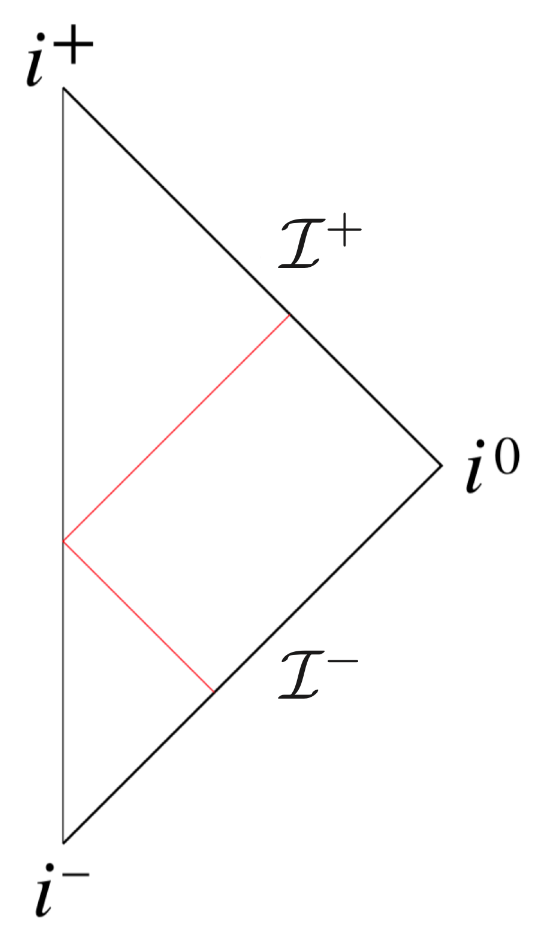
\includegraphics[width = 0.30 \textwidth]{ms-4d.png}
  \caption{Penrose diagram for $ d = 1 + 3 $ Minkowski spacetime.}
  \label{ms-4d}
\end{figure}

The corresponding Penrose diagram is drawn in Fig. \ref{ms-4d}: the spatial $ \mathbb{S}^2 $ is not shows for simplicity, but every point on the diagram corresponds to an $ \mathbb{S}^2 $ of radius $ \abs{\sin (\tilde{u} - \tilde{v})} $. The line $ \tilde{u} = \tilde{v} $ is not a boundary of Minkowski spacetime, but it's simply the origin $ r = 0 $ (at which $ \mathcal{S}^2 $ shrinks to a point): to illustrate this, a null geodesic is drawn.\\
In general, Penrose diagrams are only useful for spacetimes which contain an obvious $ \mathcal{S}^2 $, i.e. those with $ \SOn{3} $ isometry: however, these are the simplest and most important in physics.

\subsubsection{de Sitter space}

\begin{figure}
  \centering
  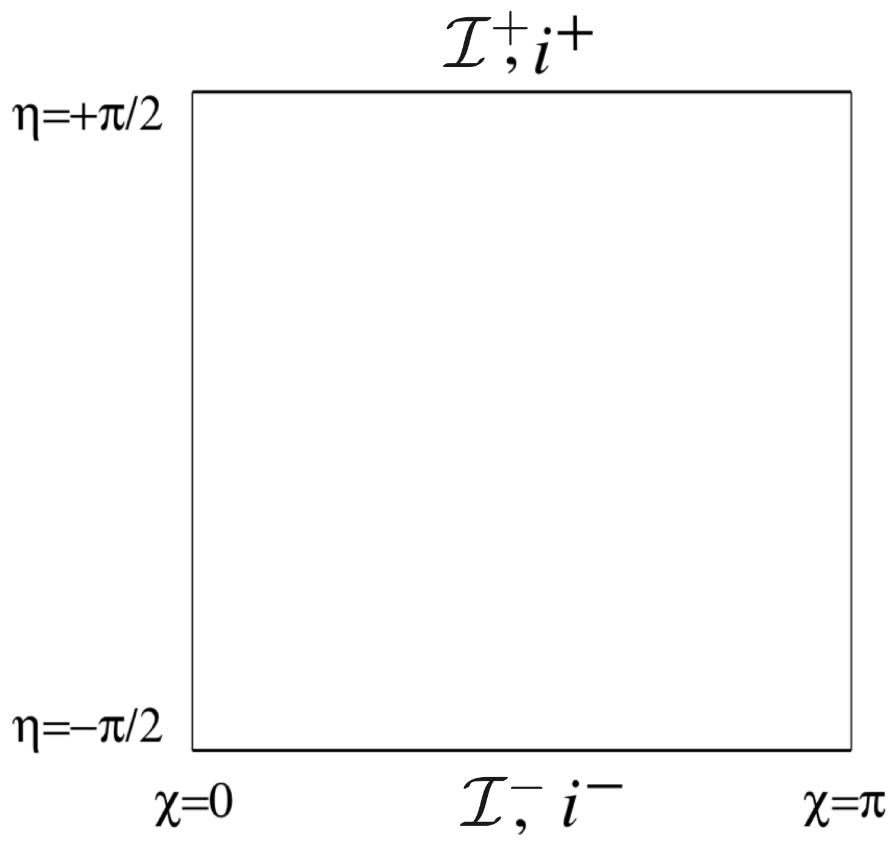
\includegraphics[width = 0.50 \textwidth]{ds-penr.png}
  \caption{Penrose diagram for de Sitter space.}
  \label{ds-penr}
\end{figure}

Recall global coordinates on dS: from Eq. \ref{eq:4.22}, $ ds^2 = -d\tau^2 + R^2 \cosh^2 \frac{\tau}{R} d\Omega_3^2 $. To draw the Penrose diagram, define \textit{conformal time} as:
\begin{equation*}
  \frac{d\eta}{d\tau} = \frac{1}{R \cosh (\tau / R)}
  \quad \Rightarrow \quad
  \cos \eta = \frac{1}{\cosh (\tau / R)}
\end{equation*}
Given that $ \tau \in \R $, then $ \eta \in \left( -\frac{\pi}{2}, +\frac{\pi}{2} \right) $. In conformal time, de Sitter space has the metric:
\begin{equation*}
  ds^2 = \frac{R^2}{\cos^2 \eta} \left( -d\eta^2 + d\Omega_3^2 \right)
\end{equation*}
Writing $ d\Omega_3^2 = d\chi^2 + \sin^2 \chi\, d\Omega_2^2 $, with $ \chi \in [0,\pi] $, de Sitter metric is conformally equivalent to:
\begin{equation*}
  d\tilde{s}^2 = -d\eta^2 + d\chi^2 + \sin^2 \chi\, d\Omega_2^2
\end{equation*}
After conformal compactification, $ \eta \in \left[ - \frac{\pi}{2}, + \frac{\pi}{2} \right] $ and $ \chi \in \left[ 0,\pi \right] $. The Penrose diagram is drawn in Fig. \ref{ds-penr}: the two vertical lines are not boundaries of dS, but simply the north and south poles of $ \mathbb{S}^3 $. The boundaries of the spacetime are the top and bottom lines, labelled both $ i^{\pm} $ and $ \mathcal{I}^{\pm} $ as they are where both timelike and null geodesics originate and terminate.

\begin{figure}
  \centering
  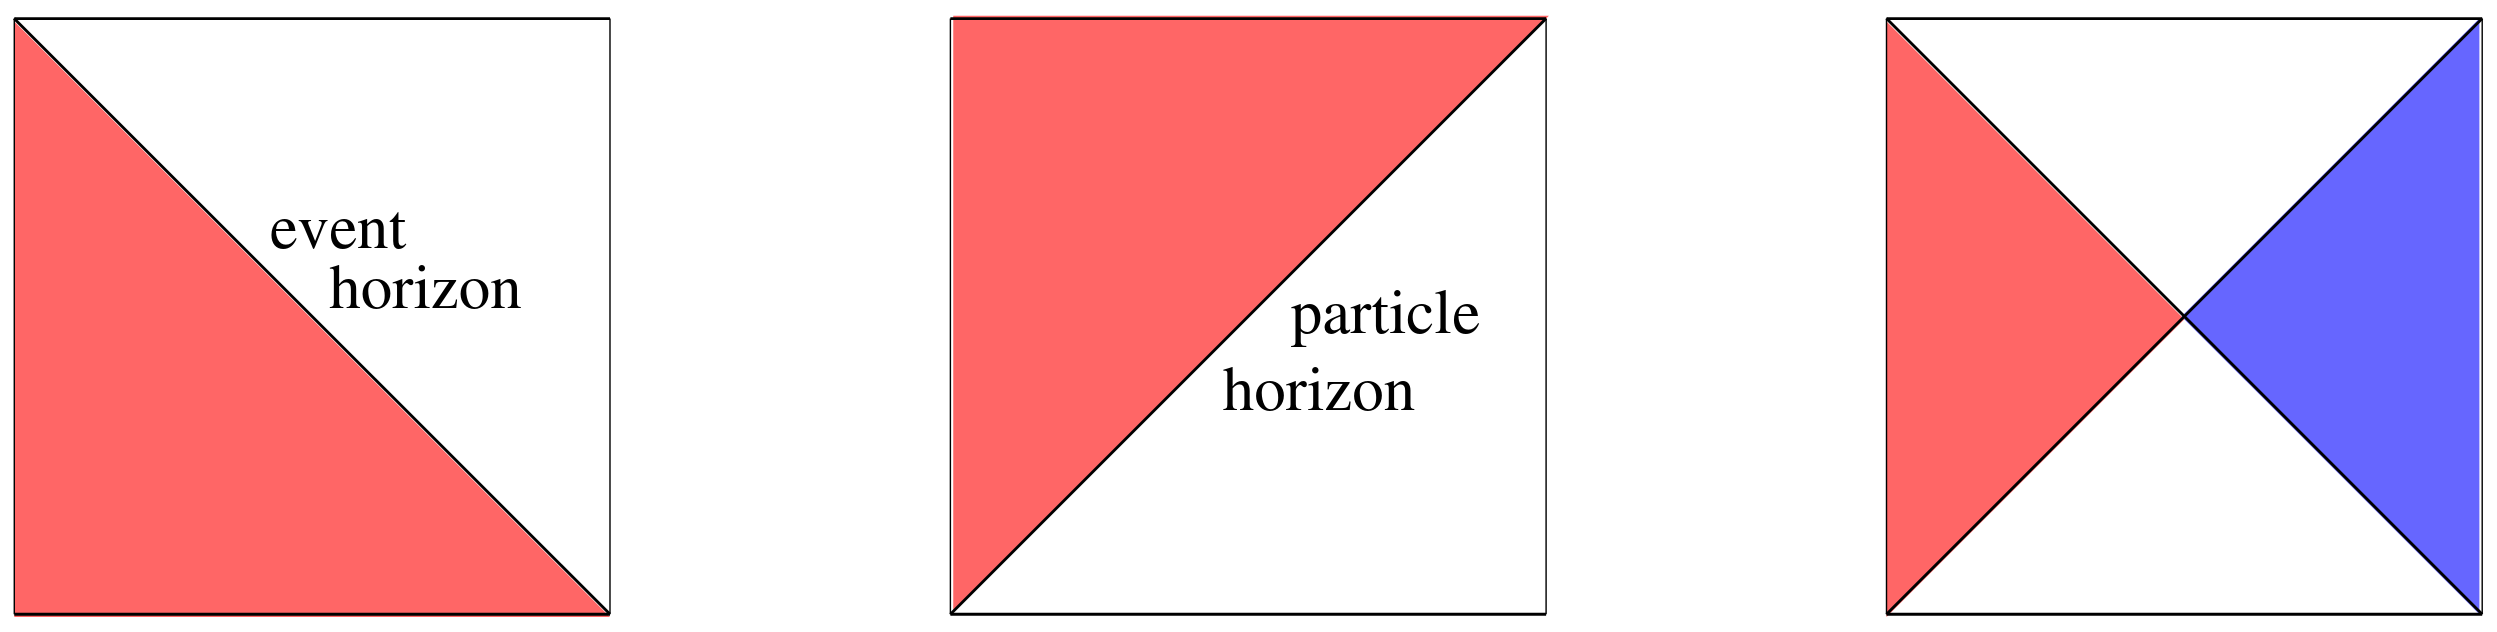
\includegraphics[width = 0.80 \textwidth]{ds-diam.png}
  \caption{Event and particle horizons for an observer at the north pole in dS, and the causal diamonds for an observer at the north and south pole.}
  \label{ds-diam}
\end{figure}

\begin{proposition}
  de Sitter spacetime has a \textit{spacelike} $ \mathbb{S}^3 $ boundary with timelike normal vector.
\end{proposition}

The causal structure of dS is very different from that of Minkowski spacetime: it is no longer true that any observer can see everything by waiting long enough. For example, as shown in Fig. \ref{ds-diam}, an observer at the north pole will eventually see only exactly half the spacetime: the boundary of this half-space is the observer's \textit{event horizon}, in the sense that signals from beyond the horizon cannot reach them. It is also clear that this event horizon is observer-dependent: in this context, these are referred to as \textit{cosmological horizons}.\\
Furthermore, an observer at the north pole will only be able to communicate with another half of the spacetime, as shown in Fig. \ref{ds-diam}: the boundary of this region of influence is known as the \textit{particle horizon} and it represents the furthest distance light can travel since the beginning of time. Its intersection with the event horizon determines the (nothern) \textit{causal diamond}: usually, nothern and southern causal diamonds are causally disconnected.\\
Penrose diagrams can also be used to explain the divergence at $ r = R $ of the metric Eq. \ref{eq:4.14} on the static patch of dS. Recalling the embedding of the static patch in $ \R^{1,4} $, parametrized as $ X^0 = \sqrt{R^2 - r^2} \sinh \frac{t}{R} $ and $ X^4 = \sqrt{R^2 - r^2} \cosh \frac{t}{R} $. Naively the surface $ r = R $ corresponds to $ X^0 = X^4 = 0 $, but writing $ r = R ( 1 - \varepsilon^2 / 2) $ yields that $ X^0 \sim R \varepsilon \sinh \frac{t}{R} $ and $ X^4 \sim R \varepsilon \cosh \frac{t}{R} $, so $ \varepsilon \rightarrow 0 $ can be obtained keeping $ X^0, X^4 \neq 0 $ and finite, provided that $ t \rightarrow \pm \infty $: to do this, $ \varepsilon \exp (\pm t / R) $ must be kept finite, thus the surface $ r = R $ is identified with the lines $ X^0 = \pm X^4 $. Translation to polar coordinates is done by $ X^0 = R \sinh \frac{\tau}{R} $ and $ X^4 = R \cosh \frac{\tau}{R} \cos \chi $, with $ \chi $ the polar angle on $ \mathbb{S}^3 $; after mapping to conformal time, one finds that:
\begin{equation*}
  X^0 = \pm X^4
  \quad \Leftrightarrow \quad
  \sin \eta = \pm \cos \chi
  \quad \Leftrightarrow \quad
  \chi = \pm \left( \eta - \frac{\pi}{2} \right)
\end{equation*}
These are precisely the lines determining the polar causal diamonds. It can also be checked that $ r = R $ on the static patch corresponds to the north pole $ \chi = 0 $ in global coordinates and that $ t = \tau $ along this line. Therefore, the static patch of dS provides coordinates that cover only the nothern causal diamond of dS spacetime, with the coordinate singularity at $ r = R $ corresponding to the past and future observer-dependent horizons.

\begin{figure}
  \centering
  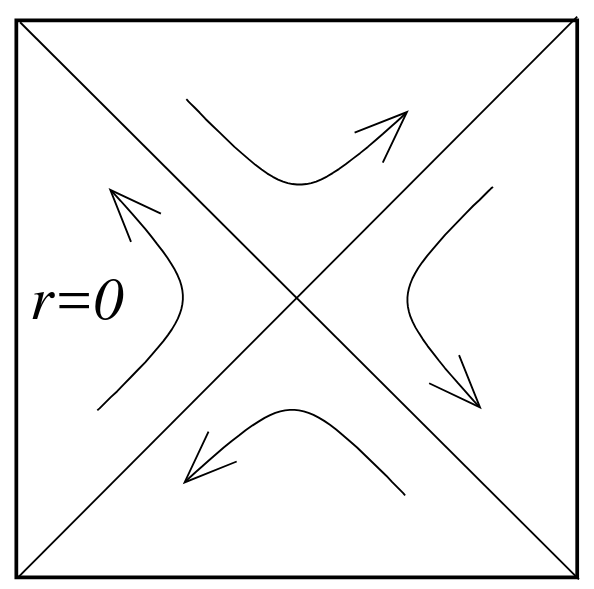
\includegraphics[width = 0.30 \textwidth]{ds-kill.png}
  \caption{$ K = \pa_t $ Killing vector field in de Sitter spacetime.}
  \label{ds-kill}
\end{figure}

Finally, Penrose diagrams help to understand the nature of the $ K = \pa_t $ Killing vector field exhibited by the static patch metric. As shown in Fig. \ref{ds-kill}, there's no global timelike Killing vector field in dS spacetime: extending the Killing vector beyond the static patch, i.e. the nothern causal diamond, it is timelike but past-oriented on the souther causal diamond and spacelike on the upper and lower quadrants.

\subsubsection{Anti-de Sitter space}

The global coordinates on AdS are, from Eq. \ref{eq:4.24}, $ ds^2 = - \cosh^2 \rho \, dt^2 + R^2 d\rho^2 + R^2 \sinh^2 \rho \, d\Omega_2^2 $, with $ \rho \in [0,\infty) $. Introduce a conformal radial coordinate:
\begin{equation*}
  \frac{d\psi}{d\rho} = \frac{1}{\cosh \rho}
  \quad \Rightarrow \quad
  \cos \psi = \frac{1}{\cosh \rho}
\end{equation*}
with $ \psi \in [0, \frac{\pi}{2}) $. With a dimensionless coordiante time $ \tilde{t} = \frac{t}{R} $, the metric becomes:
\begin{equation*}
  ds^2 = \frac{R^2}{\cos^2 \psi} \left( -d\tilde{t}^2 + d\psi^2 + \sin^2 \psi \, d\Omega_2^2 \right) = \frac{R^2}{\cos^2 \psi} \left( -d\tilde{t}^2 + d\Omega_3^2 \right)
\end{equation*}
AdS metric is conformally equivalent to:
\begin{equation*}
  d\tilde{s}^2 = -d\tilde{t}^2 + d\psi^2 + \sin^2 \psi \, d\Omega_2^2
\end{equation*}
After conformal compactification, $ \tilde{t} \in \R $ and $ \psi \in \left[ 0, \frac{\pi}{2} \right] $ and the resulting Penrose diagram is the infinite strip in Fig. \ref{ads-penr}. The edge at $ \psi = 0 $ is not a boundary, but the spatial origin where $ \mathcal{S}^2 $ shrinks to a point; in contrast, $ \psi = \frac{\pi}{2} $ is a boundary of the spacetime, labelled $ \mathcal{I} $, which should be viewed as a combination of $ \mathcal{I}^- $, $ \mathcal{I}^+ $ and $ i^0 $, since null and spacelike geodesics begin and end there.

\begin{figure}
  \centering
  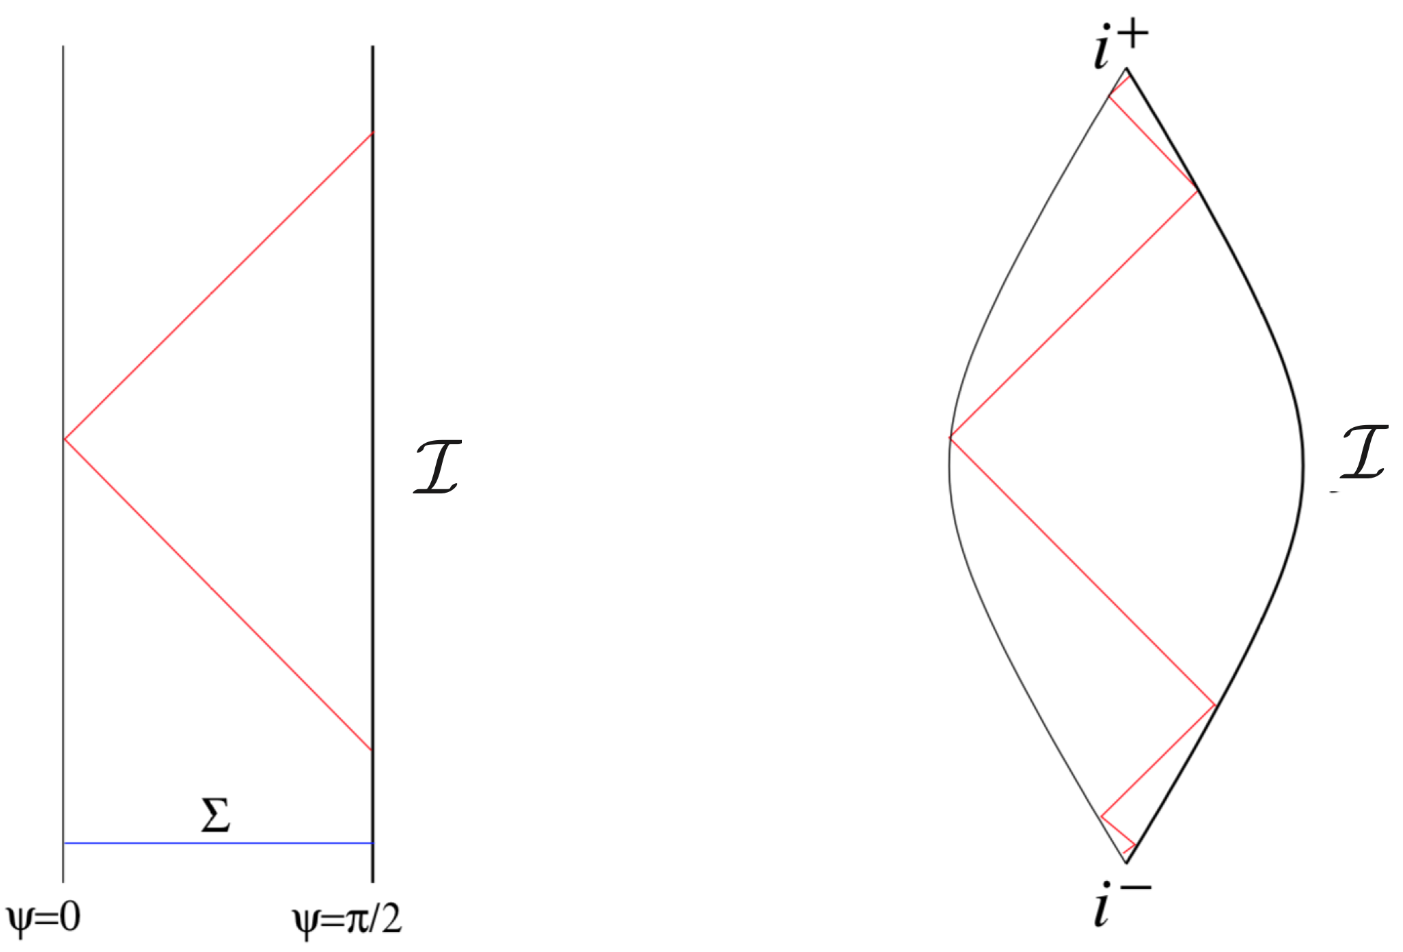
\includegraphics[width = 0.60 \textwidth]{ads-penr.png}
  \caption{Penrose diagrams for AdS, without and with conformally compactified time coordinate.}
  \label{ads-penr}
\end{figure}

\begin{proposition}
  AdS spacetime has a timelike $ \R \times \mathbb{S}^2 $ boundary with spacelike normal vector.
\end{proposition}

Note that $ \R $ is the time factor.\\
The Penrose diagram clearly shows that light rays reach the boundary in finite conformal time. To study physics in AdS, one needs to specify boundary conditions at $ \mathcal{I} $: for example, reflecting boundary conditions make light rays bounce back and forth forever, rendering AdS a $ \virgolette{box} $ spacetime in which massive particle are confined in the interior and massless particles bounce off the boundary.\\
Another characteristic of AdS space is that it isn't \textit{globally hyperbolic}: there exists no Cauchy surface on which initial data can be specified. Consider for example the 3d spacelike hypersurface $ \Sigma $ in Fig. \ref{ads-penr}. Specifying initial data on $ \Sigma $ it's not sufficient to solve for their time evolution: in AdS, there exist points in the future of $ \Sigma $ which are in causal contact with the boundary, thus the time evolution depends on boundary conditions too.\\
To make the Penrose diagram for AdS not stretch to infinity, the time coordinate can be restricted to finite values by:
\begin{equation*}
  \tilde{t} = \tan \tau
  \quad \Rightarrow \quad
  ds^2 = \frac{R^2}{\cos^2 \psi \, \cos^4 \tau} \left( -d\tau^2 + \cos^4 \tau \, d\Omega_3^2 \right)
\end{equation*}
This metric is conformally equivalent to:
\begin{equation*}
  d\tilde{s}^2 = - d\tau^2 + \cos^4 \tau \left( d\psi^2 + \sin^2 \psi \, d\Omega_2^2 \right)
\end{equation*}
with conformally compactified $ \tau \in \left[ - \frac{\pi}{2}, + \frac{\pi}{2} \right] $. Ignoring the spatial $ \mathbb{S}^2 $, the resulting Penrose diagram is drawn in Eq. \ref{ads-penr}: the spatial $ \mathbb{S}^3 $ grows and shrinks in time, the timelike boundary $ \mathcal{I} $ is still present and now the past and future timelike infinities $ i^{\pm} $ are also shown. This diagram makes it clear that a lightray bounces back and forth off teh boundary of AdS an infinite number of times.

\section{Matter coupling}

Spacetime is not merely the background on which matter exists, but it is dynamically influenced by the matter distribution on it. It is therefore necessary to study how matter couples to the spacetime metric.

\subsection{Field theories in curved spacetime}

The simplest way to describe matter is by fields governed by a Lagrangian. Consider a scalar field $ \phi(x) $. In flat Minkowski spacetime, its action is:
\begin{equation}
  \mathcal{S}_{\text{scalar}} \defeq \int d^4 x \left[ - \frac{1}{2} \eta^{\mu \nu} \pa_\mu \phi \pa_\nu \phi - V(\phi) \right]
  \label{eq:4.36}
\end{equation}
The negative sign of the kinetic term follows from the signature choice $ (-,+,+,+) $. The generalization to curved spacetime is straightforward:
\begin{equation*}
  \mathcal{S}_{\text{scalar}} = \int d^4 x \sqgm \left[ - \frac{1}{2} g^{\mu \nu} \na_\mu \phi \na_\nu \phi - V(\phi) \right]
\end{equation*}
Note the (useful) redundancy $ \na_\mu \phi = \pa_\mu \phi $. Curved spacetime also introduces the possibility to add new terms to the Lagrangian. For example:
\begin{equation}
  \mathcal{S}_{\text{scalar}} = \int d^4 x \sqgm \left[ - \frac{1}{2} \na_\mu \phi \na_\nu \phi - V(\phi) - \frac{1}{2} \xi R \phi^2 \right]
  \label{eq:4.37}
\end{equation}
for some $ \xi \in \R $. This theory correctly reduces to Eq. \ref{eq:4.36} on flat spacetime, as $ R = 0 $. To derive the equation of motion, vary the action keeping the metric fixed:
\begin{equation*}
  \begin{split}
    \delta \mathcal{S}_{\text{scalar}}
    &= \int d^4 x \sqgm \left[ - g^{\mu \nu} \na_\mu \delta \phi \na_\nu \phi - \frac{\pa V}{\pa \phi} \delta \phi - \xi R \phi \delta \phi \right] \\
    &= \int d^4 x \sqgm \left[ \left( g^{\mu \nu} \na_\mu \na_\nu \phi - \frac{\pa V}{\pa \phi} - \xi R \phi \right) \delta \phi - \na_\mu ( \delta \phi \na^\mu \phi ) \right]
  \end{split}
\end{equation*}
where integration by parts was possible due to $ \na_\mu g_{\rho \sigma} = 0 $ for the Levi-Civita connection. The last term is, by divergence theorem, a boundary term, thus the equation of motion for a scalar field theory in curved spacetime is:
\begin{equation}
  g^{\mu \nu} \na_\mu \na_\nu \phi - \frac{\pa V}{\pa \phi} - \xi R \phi = 0
  \label{eq:4.38}
\end{equation}
Now covariant derivatives are necessary, as $ \na_\mu \na_\nu \neq \pa_\mu \pa_\nu $.

\subsection{Einstein equations with matter}

To understand how matter fields back-react on spacetime, consider the combined action:
\begin{equation}
  \mathcal{S} = \frac{1}{16\pi G} \int d^4 x \sqgm \left( R - 2 \Lambda \right) + \mathcal{S}_M
  \label{eq:4.39}
\end{equation}
where $ \mathcal{S}_M $ is the action for matter fields, which in general depends on both the fields and the metric.

\begin{definition}\label{def-em-tens}
  Given a field theory for matter described by the action $ \mathcal{S}_M $, the \textit{energy-momentum tensor} is defined as:
  \begin{equation}
    T_{\mu \nu} \defeq - \frac{2}{\sqgm} \frac{\delta \mathcal{S}_M}{\delta g^{\mu \nu}}
    \label{eq:4.40}
  \end{equation}
\end{definition}

\begin{proposition}
  The energy-momentum tensor is symmetric.
\end{proposition}
\begin{proof}
  It inherits the symmetry of the metric.
\end{proof}

\begin{proposition}
  The equations of motion derived from the action Eq. \ref{eq:4.39} are:
  \begin{equation}
    G_{\mu \nu} + \Lambda g_{\mu \nu} = 8\pi G T_{\mu \nu}
    \label{eq:4.41}
  \end{equation}
\end{proposition}
\begin{proof}
  Varying the full metric, by Def. \ref{def-em-tens}:
  \begin{equation*}
    \delta \mathcal{S} = \frac{1}{16\pi G} \int d^4 x \sqgm \left[ G_{\mu \nu} + \Lambda g_{\mu \nu} \right] \delta g^{\mu \nu} - \frac{1}{2} \int d^4 x \sqgm T_{\mu \nu} \delta g^{\mu \nu} = 0
  \end{equation*}
\end{proof}

These are the full \textit{Einstein field equations}, describing gravity coupled to matter. It is possible to rewrite them by observing that the cosmological constant can be absorbed in the energy-momentum tensor as an additive component:
\begin{equation*}
  (T_\Lambda)_{\mu \nu} = - \frac{\Lambda}{8\pi G} g_{\mu \nu}
\end{equation*}
This is justified by the fact that matter fields often mimic a cosmological constant. Contracting the remaining equation with $ g^{\mu \nu} $ (i.e. taking the trace) then gives $ -R = 8\pi G T $, where $ T \equiv g^{\mu \nu} T_{\mu \nu} $, hence:
\begin{equation}
  R_{\mu \nu} = 8\pi G \left( T_{\mu \nu} - \frac{1}{2} T g_{\mu \nu} \right)
  \label{eq:4.42}
\end{equation}
Remember that the cosmological constant is present inside the energy-momentum tensor.

\subsection{Energy-momentum tensor}

The action $ \mathcal{S}_M $ is, by hypothesis, diffeomorphism-invariant, thus, recalling the argument which lead to Bianchi identity Eq. \ref{eq:4.13}, given $ \delta g_{\mu \nu} = (\ld_X g_{\mu \nu}) = 2 \na_{(\mu} X_{\nu)} $:
\begin{equation*}
  \delta \mathcal{S}_M = - \frac{1}{2} \int d^4 x \sqgm T_{\mu \nu} \delta g^{\mu \nu} = -2 \int d^4 x \sqgm T_{\mu \nu} \na^\mu X^\nu
\end{equation*}
Diffeomorphism invariance means that $ \delta \mathcal{S}_M = 0 $ for all $ X \in \xm $, hence, integrating by parts:
\begin{equation}
  \na_\mu T^{\mu \nu} = 0
  \label{eq:4.43}
\end{equation}
Of course, this was necessary to make Einstein equations consistent, as $ \na_\mu G^{\mu \nu} = 0 $. Anyway, this equation hints to the more profound nature of the energy-momentum tensor, which has nothing to do with gravity: it can be shown that the energy-momentum tensor is linked to Noether currents associated to translational invariance in space and time. Trivially, Eq. \ref{eq:4.43} reduces in flat spacetime to $ \pa_\mu T^{\mu \nu} = 0 $, which is the usual conservation law enjoyed by Noether currents.\\
Consider a translation $ x^\mu \mapsto x^\mu + \delta x^\mu $, with $ \delta x^\mu = X^\mu(x) $. The action restricted to flat spacetime is not invariant under such shift, but one which is invariant can be constructed coupling the matter fields to a background metric and allowing this to vary. The change of the action in flat space, where the metric is fixed, must be equal and opposite to the change of the action where the metric can vary but $ x^\mu $ is fixed, thus:
\begin{equation*}
  \begin{split}
    \delta \mathcal{S}_{\text{flat}}
    &= - \int d^4 x\, \frac{\delta \mathcal{S}_M}{\delta g^{\mu \nu}} \bigg\vert_{g_{\mu \nu} = \eta_{\mu \nu}} \delta g^{\mu \nu} = - \int d^4 x\, \frac{\delta \mathcal{S}_M}{\delta g^{\mu \nu}} \bigg\vert_{g_{\mu \nu} = \eta_{\mu \nu}} \pa^{(\mu} X^{\nu)} \\
    &= - 2 \int d^4 x\, \frac{\pa \mathcal{S}_M}{\pa g^{\mu \nu}} \bigg\vert_{g_{\mu \nu} = \eta_{\mu \nu}} \pa^\mu X^\nu = - 2 \int d^4 x\, \pa^\mu \left[ \frac{\pa \mathcal{S}_M}{\pa g^{\mu \nu}} \right]_{g_{\mu \nu} = \eta_{\mu \nu}} X^\nu
  \end{split}
\end{equation*}
But $ \delta \mathcal{S}_{\text{flat}} = 0 $ for all constant $ X^\mu $, as this is the definition of a translationally-invariant theory, hence the conserved Noether current in flat space is:
\begin{equation*}
  T_{\mu \nu} = - 2 \frac{\pa \mathcal{S}_M}{\pa \delta g^{\mu \nu}} \bigg\vert_{g_{\mu \nu} = \eta_{\mu \nu}}
\end{equation*}
i.e. the flat version of Eq. \ref{eq:4.40}.

\subsubsection{Field theories}

It is straightforward to compute $ T_{\mu \nu} $ for a scalar field $ \phi(x) $. Recall Eq. \ref{eq:4.37} (with $ \xi = 0 $) and Lemma \ref{lemma-sqgm}:
\begin{equation*}
  \delta \mathcal{S}_{\text{scalar}} = \int d^4 x \sqgm \left[ \frac{1}{4} g_{\mu \nu} \na^\rho \phi \na_\rho \phi + \frac{1}{2} g_{\mu \nu} V(\phi) - \frac{1}{2} \na_\mu \phi \na_\nu \phi \right] \delta g^{\mu \nu}
\end{equation*}
This gives the energy-momentum tensor:
\begin{equation}
  T_{\mu \nu} = \na_\mu \phi \na_\nu \phi - g_{\mu \nu} \left( \frac{1}{2} \pa^\rho \phi \na_\rho \phi + V(\phi) \right)
  \label{eq:4.44}
\end{equation}
Restricting to flat Minkowski spacetime:
\begin{equation*}
  T_{00} = \frac{1}{2} \dot{\phi}^2 + \frac{1}{2} (\na \phi)^2 + V(\phi)
\end{equation*}
which is the energy density of a scalar field.

\paragraph{Maxwell theory}

Varying Maxwell action Eq. \ref{eq:3.44}:
\begin{equation*}
  \delta \mathcal{S}_{\text{Maxwell}} = - \frac{1}{4} \int dx^4 \sqgm \left[ - \frac{1}{2} g_{\mu \nu} F^{\rho \sigma} F_{\rho \sigma} + 2 g^{\rho \sigma} F_{\mu \rho} F_{\nu \sigma} \right] \delta g^{\mu \nu}
\end{equation*}
So the energy-momentum tensor for Maxwell theory is:
\begin{equation}
  T_{\mu \nu} = g^{\rho \sigma} F_{\mu \rho} F_{\nu \sigma} - \frac{1}{4} g_{\mu \nu} F^{\rho \sigma} F_{\rho \sigma}
  \label{eq:4.45}
\end{equation}
In flat Minkowski spacetime:
\begin{equation*}
  T_{00} = \frac{1}{2} \ve{E}^2 + \frac{1}{2} \ve{B}^2
\end{equation*}
which is the energy density of the electromagnetic field.

\subsubsection{Perfect fluids}

A perfect fluid is described by its \textit{energy density} $ \rho(\ve{x},t) $, pressure $ p(\ve{x},t) $ and velocity 4-vector field $ u^\mu(\ve{x},t) : u^\mu u_\mu = -1 $. Pressure and energy density are related by an \textit{equation of state} $ p = p(\rho) $.

\begin{example}
  Dust is a fluid of massive particles floating around very slowly, so that the equation of state is $ p = 0 $.
\end{example}
\begin{example}
  Radiation is a fluid of photons with $ p = \rho / 3 $.
\end{example}

The energy-momentum tensor of a perfect fluid is:
\begin{equation}
  T^{\mu \nu} = (\rho + p) u^\mu u^\nu + p g^{\mu \nu}
  \label{eq:4.46}
\end{equation}
A fluid at rest ($ u^\mu = \delta_\mu,0 $) in flat Minkowski spacetime has $ T^{\mu \nu} = \diag \left( \rho, p, p, p \right) $, thus $ T_{00} $ is yet again the energy density, as expected. Generally, $ \rho = T_{\mu \nu} u^\mu u^\nu $ is the energy density measured by an observer co-moving with the fluid.\\
Bianchi identity $ \na_\mu T^{\mu \nu} = 0 $ determines two constraints. The first is:
\begin{equation}
  u^\mu \na_\mu \rho + (\rho + p) \na_\mu u^\mu = 0
  \label{eq:4.47}
\end{equation}
which is a generalization of mass conservation (where mass is identified with $ \rho $). The first term calculates how fast $ \rho $ changes along $ u^\mu $, while the second expresses it depending on the rate of flow out of the region $ \na_\mu u^\mu $. The second constraint is:
\begin{equation}
  (\rho + p) u^\mu \na_\mu u^\nu = - (g^{\mu \nu} + u^\mu u^\nu) \na_\mu p
  \label{eq:4.48}
\end{equation}
which is a generalization of Euler equation, i.e. the fluid equivalent of $ F = ma $ (or rather $ ma = F $).

\subsection{Energy conservation}

There's a difference between the energy-momentum tensor and the current which arises from a global symmetry. Consider a conserved current $ J^\mu : \na_\mu J^\mu = 0 $. Invoking the divergence theorem Eq. \ref{eq:3.41}:
\begin{equation*}
  0 = \int_V d^4 x \sqgm\, \na_\mu J^\mu = \int_{\pa V} d^3 x \sqrt{\gamma}\, n_{\mu} J^\mu
\end{equation*}
where $ V $ is a spatial volume with boundary $ \pa V = \Sigma_1 \cup \Sigma_2 \cup B $, with $ \Sigma_1, \Sigma_2 $ past and future spacelike boundarires and $ B $ timelike (lateral) boundary. If no current flows out of the region, i.e. $ n_\mu J^\mu \vert_B = 0 $, then this expression becomes the conservation $ Q(\Sigma_1) = Q(\Sigma)_2 $ of the charge associated to the current:
\begin{equation*}
  Q(\Sigma) \equiv \int_\Sigma d^3 x \sqrt{\gamma}\, n_\mu J^\mu
\end{equation*}
Thus, for a vector field, covariant conservation is equivalent to actual conservation.\\
The same argument doesn't apply to the energy-momentum tensor: the problem arises from generalizing $ \na_\mu J^\mu = \frac{1}{\sqgm} \pa_\mu (\sqgm J^\mu) $ to a higher-order tensor field, which is necessary in order to have a divergence theorem like Eq. \ref{eq:3.41}. Indeed:
\begin{equation*}
  \na_\mu T^{\mu \nu} = \pa_\mu T^{\mu \nu} + \Gamma^\mu_{\mu \rho} T^{\rho \nu} + \Gamma^\nu_{\mu \rho} T^{\mu \rho} = \frac{1}{\sqgm} \pa_\mu (\sqgm\, T^{\mu \nu}) + \Gamma^\nu_{\mu \rho} T^{\mu \rho}
\end{equation*}
The last term doesn't allow to convert the integral of $ \na_\mu T^{\mu \nu} $ to a boundary term. Instead:
\begin{equation}
  \pa_\mu (\sqgm\, T^{\mu \nu}) = -\sqgm\, \Gamma^\nu_{\mu \rho} T^{\mu \rho}
  \label{eq:4.49}
\end{equation}
Therefore, for higher-order tensors, covariant conservation is not equivalent to actual conservation.

\subsubsection{Conserved energy from Killing vectors}

Given a Killing vector $ K $, it's possible to define a conserved current associated to the energy-momentum tensor as:
\begin{equation}
  J_T^\nu \defeq - K_\mu T^{\mu \nu}
  \label{eq:4.50}
\end{equation}
This current is covariantly conserved, as:
\begin{equation*}
  \na_\nu J_T^\nu = - \left( T^{\mu \nu} \na_\nu K_\mu + K_\mu \na_\nu T^{\mu \nu} \right) = - T^{\mu \nu} \na_{(\nu} K_{\mu)} = 0
\end{equation*}
Its associated conserved charge on a spatial hypersurface $ \Sigma $ is defined as:
\begin{equation}
  Q_T(\Sigma) \defeq \int_\Sigma d^3 x \sqrt{\gamma}\, n_\mu J_T^\mu
  \label{eq:4.51}
\end{equation}
The interpretation of this charge depends on the properties of the Killing vector: if $ K $ is globally timelike, then the charge is the energy of matter $ E = Q_T(\Sigma) $, meanwhile if $ K $ is globally spacelike, then it is the momentum of matter.

\paragraph{Absence of Killing vectors}

The problem of energy conservation becomes subtle when dealing with spacetimes which do not have any globally timelike Killing vector.\\
For example, a system comprised of two orbiting stars is modelled by a spacetime which doesn't have such a Killing vector: however, the problem of matter energy conservation does not arise in this case, as the stars, while orbiting each other, emit gravitational waves, thus losing energy and eventually spiraling towards each other. Nonetheless, a meaningful question is that of energy conservation of the total system, i.e. the two stars and the gravitational field. A guess would be to consider a total energy-momentum tensor defined similarly to Eq. \ref{eq:4.40}, but:
\begin{equation*}
  T^{\text{total}}_{\mu \nu} = - \frac{2}{\sqgm} \left[ \frac{1}{16\pi G} \frac{\delta \mathcal{S}_{\text{EH}}}{\delta g^{\mu \nu}} + \frac{\delta \mathcal{S}_M}{\delta g^{\mu \nu}} \right] = - \frac{1}{8\pi G} G_{\mu \nu} + T_{\mu \nu} = 0
\end{equation*}
by Einstein field equations. This equation has no physical significance other than expressing the subtlety of energy conservation in Genera Relativity.\\
Clearly, one could try to understand the energy carried by the gravitational field alone. Unfortunately, there are compelling arguments that there exists no tensor which can be thought as the local energy density of the gravitational field: roughly speaking, the energy density of the Newtonian gravitational field $ \Phi $ is proportional to $ (\na \Phi)^2 $, so the relativistic equivalent should be proportional to the first derivatives of the metric, which can be made locally vanishing by normal coordinates due to the equivalence principle, and a tensor which vanishes in one coordinate system does so in all of them.












\chapter{Weak Gravity}
\selectlanguage{english}

Although Einstein field equations are extremely difficult to solve, a possible ansatz is to consider an almost-flat metric with $ \Lambda = 0 $, which in the so called \textit{almos-inertial coordinates} $ x^\mu $ takes the form:
\begin{equation}
  g_{\mu \nu} = \eta_{\mu \nu} + h_{\mu \nu}
  \label{eq:5.1}
\end{equation}
where the perturbation of the metric is assumed to be small: $ h_{\mu \nu} \ll 1 $.

\section{Linerarized gravity}

The aim is to expand the field equations to linear order in $ h_{\mu \nu} $: at this order, gravity can be thought as a symmetric spin 2 field $ \eta_{\mu \nu} $ propagating through flat Minkowski spacetime. Therefore, indices are raised and lowered by Minkowski metric $ \eta_{\mu \nu} = \diag \left( -1,+1,+1,+1 \right) $, and the field theory inherits Lorentz invariance:
\begin{equation*}
  x^\mu \mapsto \tensor{\Lambda}{^\mu_\nu} x^\nu
  \quad \Rightarrow \quad
  h^{\mu \nu} \mapsto \tensor{\Lambda}{^\mu_\rho} \tensor{\Lambda}{^\nu_\sigma} h^{\rho \sigma} (\Lambda^{-1} x)
\end{equation*}
where $ \eta^{\mu \nu} = \eta^{\mu \rho} \eta^{\nu \sigma} h_{\rho \sigma} $. To leading order, the inverse metric is $ g^{\mu \nu} = \eta^{\mu \nu} - h^{\mu \nu} $, thus:
\begin{equation}
  \Gamma^\sigma_{\nu \rho} = \frac{1}{2} \eta^{\sigma \lambda} \left( \pa_\nu h_{\lambda \rho} + \pa_\rho h_{\nu \lambda} - \pa_\lambda h_{\nu \rho} \right)
  \label{eq:5.2}
\end{equation}
Recalling Eq. \ref{eq:3.36}, the $ \Gamma \Gamma \sim h^2 $ terms of the Riemann tensor are negligible to first order, so:
\begin{equation}
  \tensor{R}{^\sigma_{\rho \mu \nu}} = \frac{1}{2} \eta^{\sigma \lambda} \left( \pa_\mu \pa_\rho h_{\nu \lambda} - \pa_\mu \pa_\lambda h_{\nu \rho} - \pa_\nu \pa_\rho h_{\mu \lambda} + \pa_\nu \pa_\lambda h_{\mu \rho} \right)
  \label{eq:5.3}
\end{equation}
Contracting $ (\sigma,\rho) $, the Ricci tensor is:
\begin{equation}
  R_{\mu \nu} = \frac{1}{2} \left( \pa^\rho \pa_\mu h_{\nu \rho} + \pa^\rho \pa_\nu h_{\mu \rho} - \Box h_{\mu \nu} - \pa_\mu \pa_\nu h \right)
  \label{eq:5.4}
\end{equation}
where $ \Box \defeq \pa^\mu \pa_\mu $ and $ h = \tensor{h}{^\mu_\mu} $ is the trace of $ h_{\mu \nu} $. The Ricci scalar is:
\begin{equation}
  R = \pa^\mu \pa^\nu h_{\mu \nu} - \Box h
  \label{eq:5.5}
\end{equation}
Finally, the Einstein tensor can be expressed as:
\begin{equation}
  G_{\mu \nu} = \frac{1}{2} \left[ \pa^\rho \pa_\mu h_{\nu \rho} + \pa^\rho \pa_\nu h_{\mu \rho} - \Box h_{\mu \nu} - \pa_\mu \pa_\nu h - \left( \pa^\rho \pa^\sigma h_{\rho \sigma} - \Box h \right) \eta_{\mu \nu} \right]
  \label{eq:5.6}
\end{equation}
For linearized gravity, Bianchi identity $ \na^\mu G_{\mu \nu} = 0 $ becomes $ \pa^\mu G_{\mu \nu} = 0 $, which is indeed obeyed by Eq. \ref{eq:5.6}. Einstein field equations with a source $ T_{\mu \nu} $, which, for consistency, must be suitably small, are then a set of linear PDEs:
\begin{equation}
  \pa^\rho \pa_\mu h_{\nu \rho} + \pa^\rho \pa_\nu h_{\mu \rho} - \Box h_{\mu \nu} - \pa_\mu \pa_\nu h - \left( \pa^\rho \pa^\sigma h_{\rho \sigma} - \Box h \right) \eta_{\mu \nu} = 16\pi G T_{\mu \nu}
  \label{eq:5.7}
\end{equation}
This can be thought as $ \mathfrak{L}(h_{\mu \nu}) = 16\pi G T_{\mu \nu} $, where $ \mathfrak{L} $ is a linear differential operator known as \textit{Lichnerowicz operator}.

\begin{proposition}
  Eq. \ref{eq:5.7} are the equations of motion derived from the \textit{Fierz-Pauli action}:
  \begin{equation}
    \mathcal{S}_{\text{FP}} = \frac{1}{8\pi G} \int d^4 x \left[ - \frac{1}{4} \pa_\rho h_{\mu \nu} \pa^\rho h^{\mu \nu} + \frac{1}{2} \pa_\rho h_{\mu \nu} \pa^\nu h^{\rho \mu} + \frac{1}{4} \pa_\mu h \pa^\mu h - \frac{1}{2} \pa_\nu h^{\mu \nu} \pa_\mu h \right]
    \label{eq:5.8}
  \end{equation}
\end{proposition}
\begin{proof}
  Varying the action:
  \begin{equation*}
    \begin{split}
      \delta \mathcal{S}_{\text{FP}}
      &= \frac{1}{8\pi G} \int d^4 x \left[ \frac{1}{2} \pa_\rho \pa^\rho h_{\mu \nu} - \pa^\rho \pa_\nu h_{\rho \mu} - \frac{1}{2} \eta_{\mu \nu} \pa^\rho \pa_\rho h + \frac{1}{2} \pa_\nu \pa_\mu h + \frac{1}{2} \eta_{\mu \nu} \pa_\rho \pa_\sigma h^{\rho \sigma} \right] \delta h^{\mu \nu} \\
      &= \frac{1}{8\pi G} \int d^4 x \left[ - G_{\mu \nu} \delta h^{\mu \nu} \right]
    \end{split}
  \end{equation*}
  Hence, $ G_{\mu \nu} = 0 $. To get the matter coupling, add $ T_{\mu \nu} h^{\mu \nu} $ to the action.
\end{proof}

\subsection{Gauge symmetry}

Linearized gravity inherits a useful gauge symmetry from the diffeomorphism invariance of the full theory. Under a change of coordinates $ x^\mu \mapsto x^\mu - \xi^\mu(x) $, where $ \xi(x) $ is assumed to be small, the metric changes by Eq. \ref{eq:4.11} as $ \delta g_{\mu \nu} = (\ld_\xi g)_{\mu \nu} = \na_\mu \xi_\nu + \na_\nu \xi_\mu $; for the linearized metric Eq. \ref{eq:5.1}, being both $ h $ and $ \xi $ small, the covariant derivatives take the vanishing connection of Minkowski spacetime, thus:
\begin{equation}
  h_{\mu \nu} \mapsto h_{\mu \nu} + \pa_\mu \xi_\nu + \pa_\nu \xi_\mu
  \label{eq:5.9}
\end{equation}
This is similar to the gauge transformation of Maxwell theory $ A_\mu \mapsto A_\mu + \pa_\mu \alpha $: just like $ F_{\mu \nu} = 2 \pa_{[\mu} A_{\nu]} $ is gauge-invariant, so is the linearized Riemann tensor Eq. \ref{eq:5.3}.

\begin{proposition}
  The Fierz-Pauli action is invariant under the gauge symmetry Eq. \ref{eq:5.9}.
\end{proposition}
\begin{proof}
  Recalling the linearized Bianchi identity $ \pa^\mu G_{\mu \nu} = 0 $:
  \begin{equation*}
    \delta \mathcal{S}_{\text{FP}} = - \frac{1}{8\pi G} \int d^4 x\, 2 G_{\mu \nu} \pa^\mu \xi^\nu = \frac{1}{4\pi G} d^4 x\, \pa^\mu G_{\mu \nu} \xi^\nu = 0
  \end{equation*}
\end{proof}

As in Electromagnetism, it's useful to impose a gauge fixing condition.

\begin{proposition}
  It's always possible to pick \textit{de Donder gauge}:
  \begin{equation}
    \pa^\mu h_{\mu \nu} - \frac{1}{2} \pa_\nu h = 0
    \label{eq:5.10}
  \end{equation}
\end{proposition}
\begin{proof}
  Suppose that the doesn't obey de Donder condition, but WLOG $ \pa^\mu h_{\mu \nu} - \frac{1}{2} \pa_\nu h = f_\nu $ for some functions $ f_\nu $. After the gauge transformation Eq. \ref{eq:5.9}, this becomes $ \pa^\mu h_{\mu \nu} - \frac{1}{2} \pa_\nu h + \Box \xi_\nu = f_\nu $, thus one only needs to find $ \xi_\nu : \Box \xi_\nu = f_\nu $, which always has a solution.
\end{proof}

In de Donder gauge, the field equations Eq. \ref{eq:5.7} are greatly simplified:
\begin{equation}
  \Box h_{\mu \nu} - \frac{1}{2} \eta_{\mu \nu} \Box h = -16\pi G T_{\mu \nu}
  \label{eq:5.11}
\end{equation}
To simplify these equations even more, it's useful to define:
\begin{equation*}
  \bar{h}_{\mu \nu} \equiv h_{\mu \nu} - \frac{1}{2} \eta_{\mu \nu} h
  \quad \Rightarrow \quad
  h_{\mu \nu} = \bar{h}_{\mu \nu} - \frac{1}{2} \eta_{\mu \nu} \bar{h}
\end{equation*}
as $ \bar{h} = - h $. With this choice, the linearized Einstein equations in de Donder gauge reduce to a set of wave equations:
\begin{equation}
  \Box \bar{h}_{\mu \nu} = -16\pi G T_{\mu \nu}
  \label{eq:5.12}
\end{equation}

\paragraph{Non-linear theory}

de Donder gauge can be extended to the full non-linear theory as the condition:
\begin{equation}
  g^{\mu \nu} \Gamma^\rho_{\mu \nu} = 0
  \label{eq:5.13}
\end{equation}
Note that this isn't a tensor equation, as $ \Gamma^\rho_{\mu \nu} $ isn't a tensor, and indeed the point of gauge fixing is to set a preferred choice of coordinates. This gauge condition simplifies the expression of the d'Alembertian $ \Box \defeq \na^\mu \na_\mu = g^{\mu \nu} ( \pa_\mu \pa_\nu - \Gamma^\rho_{\mu \nu} \pa_\rho ) $, which simply becomes $ \Box = g^{\mu \nu} \pa_\mu \pa_\nu $; moreover, the same applies to 1-forms: $ \na^\mu \omega_\mu = g^{\mu \nu} \na_\mu \omega_\nu = g^{\mu \nu} ( \pa_\mu \omega _\nu - \Gamma^\rho_{\mu \nu} \omega_\rho ) = \pa^\mu \omega_\mu $.

\subsection{Newtonian limit}

In the presence of a low-density, slowly-moving distribution of matter, the linearized field equations reduce to the Newtonian theory of gravity. For a stationary matter configuration, the only non-vanishing component of the energy-momentum tensor is $ T_{00} = \rho(\ve{x}) $; moreover, since there's no time-dependence, $ \Box = -\pa_t^2 + \na^2 = \na^2 $. The Einstein equations become:
\begin{equation*}
  \na^2 \bar{h}_{00} = -16\pi G \rho(\ve{x})
  \qquad
  \na^2 \bar{h}_{0i} = \na^2 \bar{h}_{ij} = 0
\end{equation*}
With suitable boundary conditions, the solutions to these equations are:
\begin{equation*}
  \bar{h}_{00} = -4 \Phi(\ve{x})
  \qquad
  \bar{h}_{0i} = \bar{h}_{ij} = 0
\end{equation*}
where $ \Phi : \na^2 \Phi = 4\pi G \rho $ is the Newtonian gravitational potential. Then $ \bar{h} = 4 \Phi $ and:
\begin{equation*}
  h_{\mu \nu} = -2\Phi(\ve{x}) \delta_{\mu \nu}
\end{equation*}
The full metric $ g_{\mu \nu} = \eta_{\mu \nu} + h_{\mu \nu} $ it thus expressed as:
\begin{equation*}
  ds^2 = - \left( 1 + 2\Phi(\ve{x}) \right) dt^2 + \left( 1 - 2\Phi(\ve{x}) \right) d\ve{x}^2
\end{equation*}
This is exactly teh condition Eq. \ref{eq:1.29}. Interestingly, for a point particle $ \Phi(\ve{x}) = - \frac{GM}{r} $ and the metric coincides with the leading expansion of Schwarzschild metric (the $ g_{00} $ term is exact).

\section{Gravitational waves}

To study the propagation of gravitational waves in vacuum and in the absence of sources, one needs to solve the linearized wave equation:
\begin{equation}
  \Box \bar{h}_{\mu \nu} = 0
  \label{eq:5.14}
\end{equation}
A possible solution is the gravitational wave:
\begin{equation}
  \bar{h}_{\mu \nu}(x) = \Re \{ H_{\mu \nu} e^{i k_\rho x^\rho} \}
  \label{eq:5.15}
\end{equation}
where $ H_{\mu \nu} \in \C^{4 \times 4} $ is a symmetric polarization matrix and the wave-vector $ k^\mu $ is a real 4-vector. For simplicity, the $ \Re $ is made implicit in the following calculations. This plane wave ansatz solves Eq. \ref{eq:5.14} if the wave-vector is null:
\begin{equation}
  k_\mu k^\mu = 0
  \label{eq:5.16}
\end{equation}
Therefore, gravitational waves propagate at the speed of light. Writing $ k^\mu = (\omega, \ve{k}) $, this condition becomes $ \omega = \pm \abs{\ve{k}} $. Moreover, being the vacuum wave equation linear, the general solution is just a linear combination of plane waves.\\
The polarization matrix has 10 components, but gauge conditions are yet to be imposed. The plane wave ansatz satisfies de Donder gauge condition $ \pa^\mu \bar{h}_{\mu \nu} = 0 $ only if:
\begin{equation}
  k^\mu  H_{\mu \nu} = 0
  \label{eq:5.17}
\end{equation}
The polarization is then transverse to the direction of propagation. Furthermore, de Donder gauge still allows for gauge transformations $ h_{\mu \nu} \mapsto h_{\mu \nu} \pa_\mu \xi_\nu + \pa_\nu \xi_\mu $, i.e. $ \bar{h}_{\mu \nu} \mapsto \bar{h}_{\mu \nu} + \pa_\mu \xi_\nu + \pa_\nu \xi_\mu - \eta_{\mu \nu} \pa^\rho \xi_\rho $, so the solution is still in de Donder gauge only if:
\begin{equation*}
  \Box \xi_\mu = 0 \quad \Rightarrow \quad \xi_\mu(x) = \lambda_\mu e^{i k_\rho x^\rho}
\end{equation*}
This gauge transformation shifts the polarization matrix as:
\begin{equation}
  H_{\mu \nu} \mapsto H_{\mu \nu} + i \left( k_\mu \lambda_\nu + k_\nu \lambda_\mu - \eta_{\mu \nu} k^\rho \lambda_\rho \right)
  \label{eq:5.18}
\end{equation}
Polarization matrices which differ by this term thus describe the same gravitational wave. Hence, it is possible to choose $ \lambda_\mu $ in order to have:
\begin{equation}
  H_{0 \mu} = 0 \quad \land \quad \tensor{H}{^\mu_\mu} = 0
  \label{eq:5.19}
\end{equation}
These condition, together with Eq. \ref{eq:5.17}, are called \textit{transverse traceless gauge}. Being $ H_{\mu \nu} $ traceless, in this gauge $ \bar{h}_{\mu \nu} = h_{\mu \nu} $, as it is traceless too. Of the 10 components of the polarization matrix, only 2 are independent: de Donder condition Eq. \ref{eq:5.17} poses 4 constraints and the gauge transformation Eq. \ref{eq:5.18} poses 4 more of them. Therefore, there are only two independent polarizations in $ H_{\mu \nu} $.

\begin{example}
  Consider a gravitational wave propagating in the $ z $ direction: $ k^\mu = (\omega,0,0,\omega) $, thus $ H_{0 \nu} + H_{3 \nu} = 0 $ by Eq. \ref{eq:5.17}. By Eq. \ref{eq:5.19}, the polarization matrix is then restricted to be:
  \begin{equation}
    H_{\mu \nu} =
    \begin{bmatrix}
      0 & 0 & 0 & 0 \\
      0 & H_+ & H_\times & 0 \\
      0 & H_\times & -H_+ & 0 \\
      0 & 0 & 0 & 0
    \end{bmatrix}
    \label{eq:5.20}
  \end{equation}
  where in general $ H_+, H_\times \in \C $. The two polarizations are seen explicitly.
\end{example}

\subsection{Polarizations}

Point particles moving along geodesics are not affected by gravitational waves due to the equivalence principle: to measure their passage, one needs to study how the relative distance between two observers changes, which is done using the geodesic deviation (recall Sec. \ref{sec-geo-dev}).\\
Consider a family of geodesics $ x^\mu(\tau,s) $ with tangent vector field $ u^\mu = \pa_\tau \vert_s x^\mu $ and deviation vector field $ S^\mu = \pa_s \vert_\tau x^\mu $. The geodesic deviation equation (Eq. \ref{eq:3.58}) reads:
\begin{equation*}
  \frac{D^2 S^\mu}{D \tau^2} = \tensor{R}{^\mu_{\rho \sigma \nu}} u^\rho u^\sigma S^\nu
\end{equation*}
Suppose that, in the absence of gravitational waves, the geodesics are in a rest-frame such that $ u^\mu = (1,0,0,0) $: as the gravitational wave passes $ u^\mu = (1,0,0,0) + o(h) $, so the aim is to compute the geodesic deviation to leading order in $ h $. The Riemann tensor is already $ o(h) $, thus other correction terms can be neglected; similarly, proper time $ \tau $ can be replaced with coordinate time $ t $, so that the geodesic deviation equation becomes:
\begin{equation*}
  \frac{d^2 S^\mu}{dt^2} = \tensor{R}{^\mu_{00 \nu}} S^\nu
\end{equation*}
In the linearized regime, the Riemann tensor is given by Eq. \ref{eq:5.3}, hence, using $ h_{\mu 0} = 0 $, the needed components are $ \tensor{R}{^\mu_{00 \nu}} = \frac{1}{2} \pa_0^2 \tensor{h}{^\mu_\nu} $ and:
\begin{equation}
  \frac{d^2 S^\mu}{dt^2} = \frac{1}{2} \frac{d^2 \tensor{h}{^\mu_\nu}}{dt^2} S^\nu
  \label{eq:5.21}
\end{equation}
For simplicity, consider a wave propagating in the $ z $ direction with polarization matrix Eq. \ref{eq:5.20} and solve the geodesic deviation equation in the $ z = 0 $ plane only, as $ S^0 $ and $ S^3 $ are not affected by the gravitational wave.

\subsubsection{$ + $ polarization}

Setting $ H_\times = 0 $, Eq. \ref{eq:5.21} becomes:
\begin{equation*}
  \frac{d^2 S^1}{dt^2} = - \frac{\omega^2}{2} H_+ e^{i \omega t} S^1
  \qquad \qquad
  \frac{d^2 S^2}{dt^2} = + \frac{\omega^2}{2} H_+ e^{i \omega t} S^2
\end{equation*}
Solving perturbatively in $ H_+ $, at leading order:
\begin{equation}
  S^1(t) = S^1(0) \left[ 1 + \frac{1}{2} H_+ e^{i \omega t} + \dots \right]
  \qquad
  S^2(t) = S^2(t) \left[ 1 - \frac{1}{2} H_+ e^{i \omega t} + \dots \right]
  \label{eq:5.22}
\end{equation}
where, again, the $ \Re $ is implicit (recall that in general $ H_+ \in \C $). To visualize these solutions, consider a family of neighbouring geodesics which, at $ t = 0 $, are arranged around a circle of radius $ R $: the initial conditions then satisfy $ S^1(0)^2 + S^2(0)^2 = R^2 $. The relative negative sign determines:

\begin{figure*}[h]
  \centering
  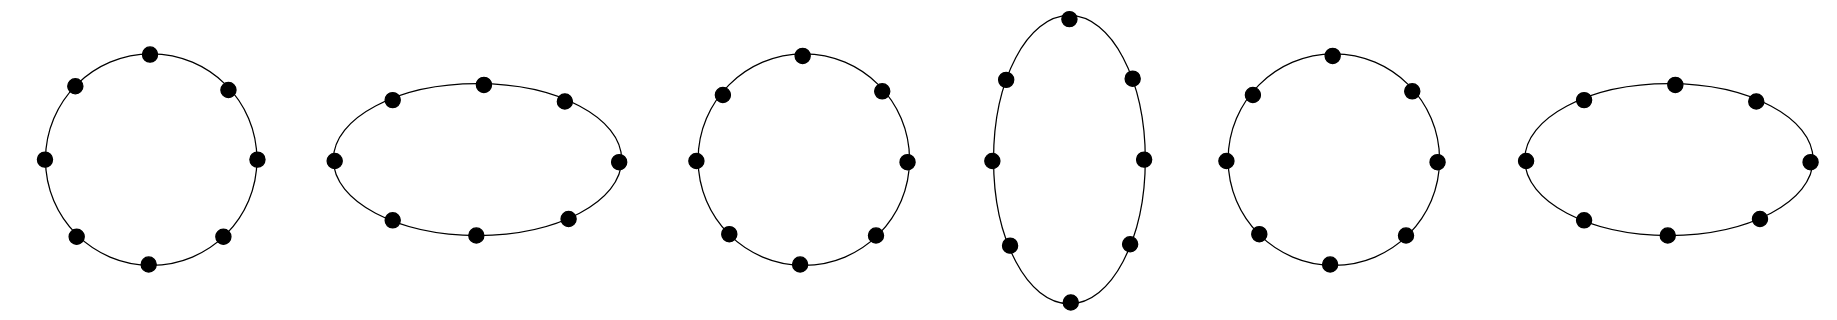
\includegraphics[width = 0.65 \textwidth]{gw-p.png}
\end{figure*}

\subsubsection{$ \times $ polarization}

Setting $ H_\times = 0 $, Eq. \ref{eq:5.21} becomes:
\begin{equation*}
  \frac{d^2 S^1}{dt^2} = - \frac{\omega^2}{2} H_\times e^{i \omega t} S^2
  \qquad \qquad
  \frac{d^2 S^2}{dt^2} = - \frac{\omega^2}{2} H_\times e^{i \omega t} S^1
\end{equation*}
Solving perturbatively in $ H_\times $, at leading order:
\begin{equation}
  S^1(t) = S^1(0) + \frac{1}{2} S^2(0) H_\times e^{i \omega t} + \dots
  \qquad
  S^2(t) = S^2(t) + \frac{1}{2} S^1(0) H_\times e^{i \omega t} + \dots
  \label{eq:5.23}
\end{equation}
This is the same displacement as Eq. \ref{eq:5.22}, but rotated by 45°: to see this, note that $ S^1(t) \pm S^2(t) $ have the same functional expression as Eq. \ref{eq:5.22}. Thus:

\begin{figure*}[h]
  \centering
  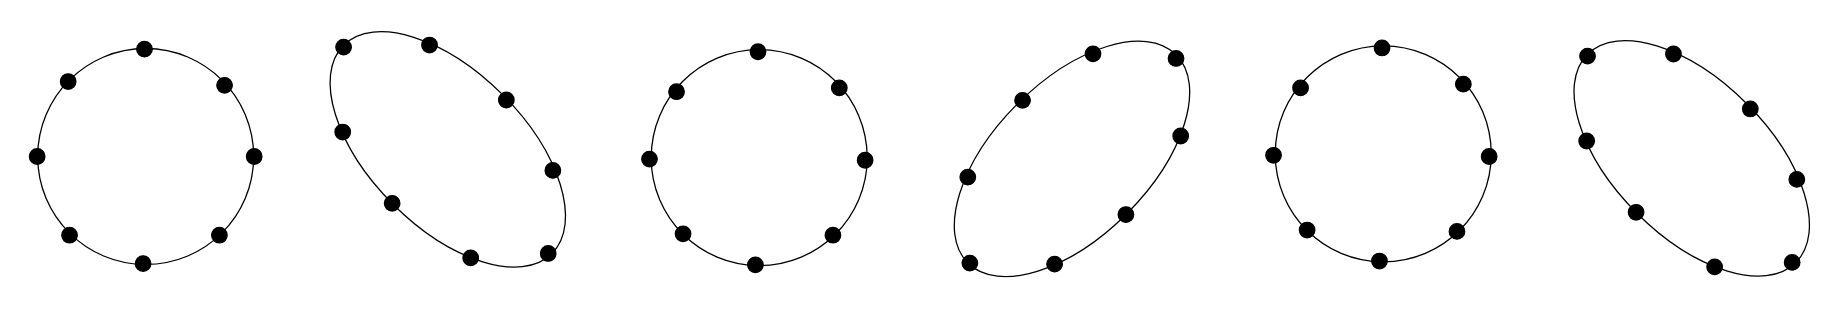
\includegraphics[width = 0.65 \textwidth]{gw-t.png}
\end{figure*}

The general polarization is a linear combination of both: the result is yet an elliptic displacement whose axes rotate, analogously to the circular polarization of light. Interestingly, note that displacements due to gravitational waves are invariant under $ \pi $ rotations, while light polarization, being described by a vector, is invariant under $ 2\pi $ rotations: this reflects the fact that the graviton has spin 2 and the photon has spin 1.

\subsubsection{Gravitational wave detection}

Gravitational wave detectors are interferometers, which bounce light back and forth between two arms. If the gravitational wave propagates perpendicular to the plane of detection, it will shorten one arm and lengthen the other: assuming the arms are aligned with $ x $ and $ y $ axes, the maximum change in length by Eq. \ref{eq:5.22} is $ L' = L (1 \pm H_+ / 2) $, i.e. $ \delta L / L = H_+ / 2 $.
For a typical astrophysical source $ H_+ \sim 10^{-21} $, while for LIGO $ L \sim 3\,\text{km} $, thus $ \delta L \sim 10^{-18} \,\text{m} $: this is smaller than the radius of the proton and extremely difficult to detect, however the first direct measurement of gravitational waves was performed in 2015 and now LIGO and VIRGO detectors have observed a large number of mergers involving black holes and neutron stars.

\begin{figure}[h]
  \centering
  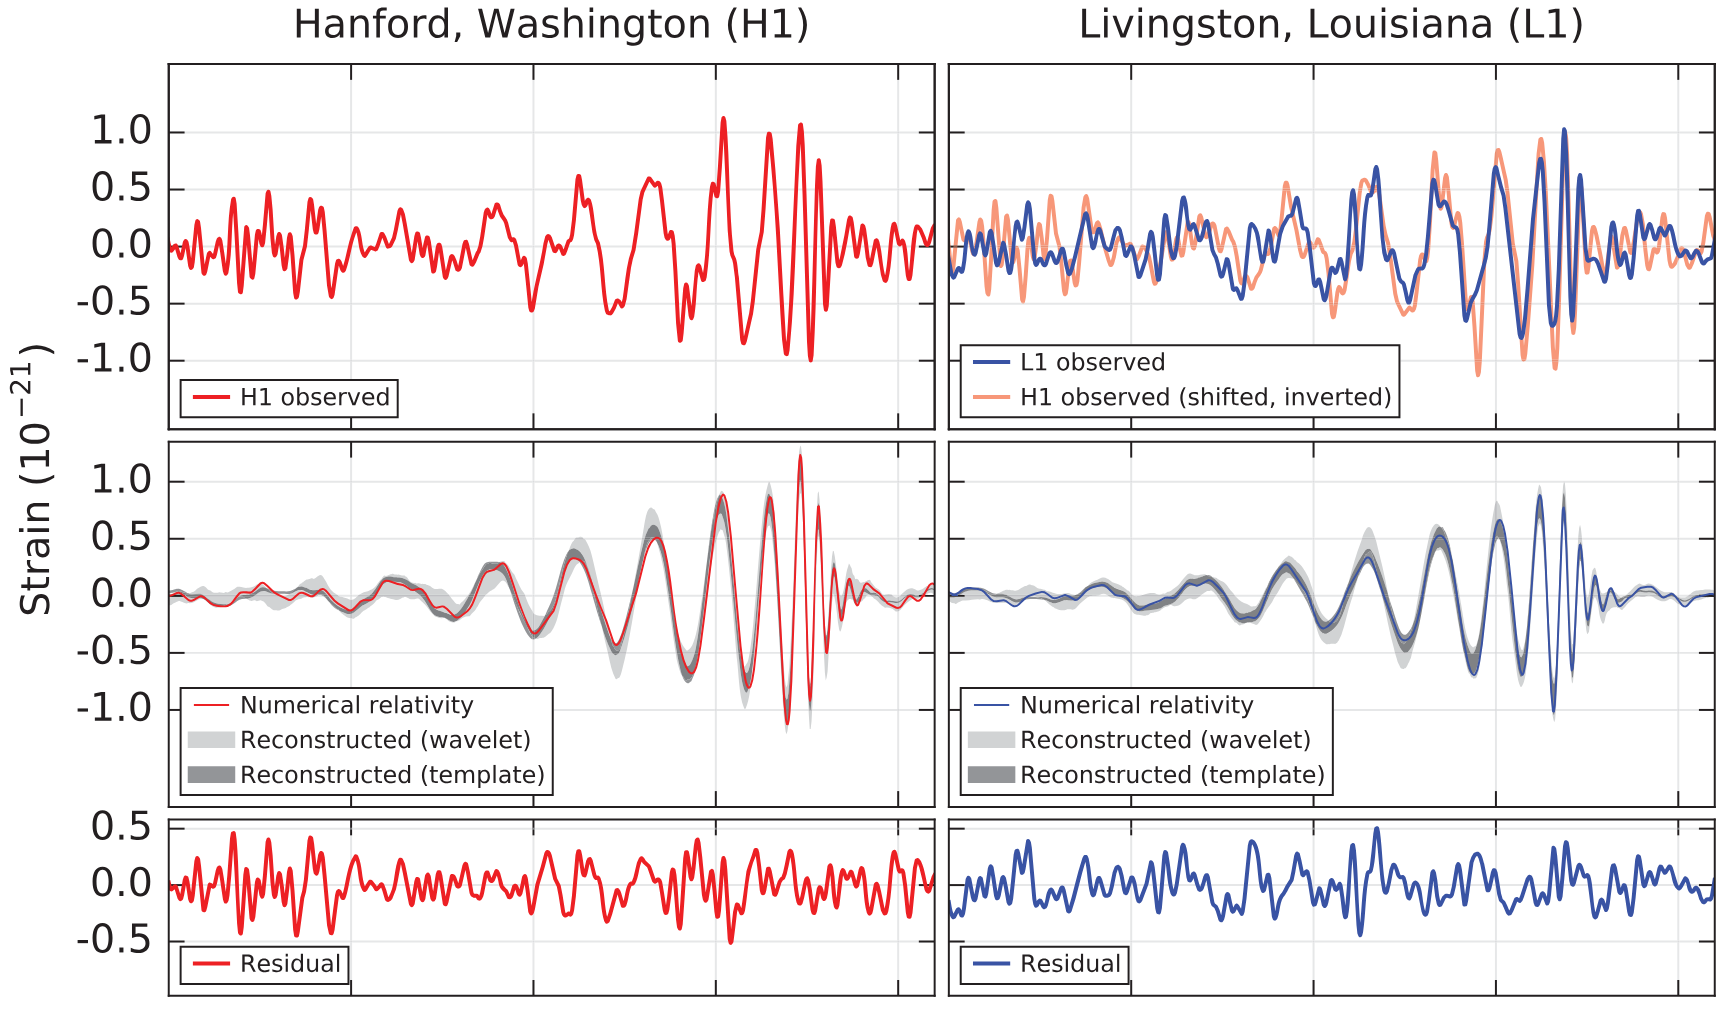
\includegraphics[width = 0.45 \textwidth]{ligo.png}
  \caption{First detection of gravitational waves by LIGO.}
  \label{ligo}
\end{figure}

\subsection{Exact solutions}

Given the found wave-like solution to the linearized field equations, the metric of a wave moving in the positive $ z $ direction takes the form:
\begin{equation}
  ds^2 = -dt^2 + \left( \delta_{ab} + h_{ab}(z - t) \right) dx^a dx^b + dz^2
  \label{eq:5.24}
\end{equation}
with $ a,b = 1,2 $. Being the wave equation linear, any function $ h_{ab}(z - t) $ is a solution: Eq. \ref{eq:5.15} is simply the Fourier decomposition of the general solution.\\
The extreme weakness of gravitational waves makes the linearized metric Eq. \ref{eq:5.1} suitable to describe their properties. However, the wave solution has an extension to the general non-linear field equations. Consider a wave propagating in the positive $ z $ direction and introduce lightcone coordinates:
\begin{equation*}
  u = t - z
  \qquad
  v = t + z
\end{equation*}
Then, consider the plane wave ansatz, also called \textit{Brinkmann metric}:
\begin{equation*}
  ds^2 = -du\,dv + dx^a dx^a + H_{ab}(u) x^a x^b du^2
\end{equation*}
Note that to obtain the linearized metric Eq. \ref{eq:5.24} from Brinkmann metric, one needs some change of coordinates. It is possible to show that Brinkmann metric is Ricci flat for any traceless matrix $ H_{ab}(u) $, hence solving the vacuum Einstein equations:
\begin{equation*}
  R_{\mu \nu} = 0 \quad \Leftrightarrow \quad \tensor{H}{^a_a}(u) = 0 \quad \Leftrightarrow \quad H_{ab}(u) =
  \begin{bmatrix}
    H_{11}(u) & H_{12}(u) \\
    H_{12}(u) & -H_{11}(u)
  \end{bmatrix}
\end{equation*}
The general metric has again two independent polarization states.

\section{Perturbing spacetime}

The gravitational plane wave solution Eq. \ref{eq:5.15} is not realistic, as it is comes from infinity and goes to infinity: in reality, gravitational waves are produced at some point and radiate out. The analogy with Electromagnetism persists: as electromagnetic waves are produced by oscillating charges, gravitational waves are produced by oscillating masses.

\subsection{Green's function}

Recall the linearized Einstein field equations Eq. \ref{eq:5.12}:
\begin{equation*}
  \Box \bar{h}_{\mu \nu} = -16\pi G T_{\mu \nu}
\end{equation*}
which assumes that both $ h_{\mu \nu} $ and $ T_{\mu \nu} $ are small. These are a set of decoupled wave equations.\\
Consider a matter field localized in a spatial region $ \Sigma $, in which a time-dependent energy-momentum source $ T_{\mu \nu}(\ve{x},t) $ is present (ex.: two orbiting black holes): the localization condition then is simply $ T_{\mu \nu}(\ve{x},t) = 0 \,\forall \ve{x} \notin \Sigma $. The question is what the metric $ h_{\mu \nu} $ looks like far away from $ \Sigma $. The solution to Eq. \ref{eq:5.12} outside of $ \Sigma $ can be expressed using the retarded Green's function:
\begin{equation}
  \bar{h}_{\mu \nu}(\ve{x},t) = 4G \int_\Sigma d^3 x'\, \frac{T_{\mu \nu}(\ve{x}',t_r)}{\abs{\ve{x} - \ve{x}'}}
  \qquad t_r \equiv t - \abs{\ve{x} - \ve{x}'}
  \label{eq:5.25}
\end{equation}
Retarded time expresses the causality of the wave equation. This solution satisfies de Donder condition $ \pa^\mu \bar{h}_{\mu \nu} = 0 $ only if $ \pa^\mu T_{\mu \nu} = 0 $, i.e. the energy-momentum tensor is conserved; however, it does not automatically satisfy conditions Eq. \ref{eq:5.19}.\\
Denoting the size of $ \Sigma $ as $ d $ and $ r \equiv \abs{x} $, then approximating:
\begin{equation*}
  \abs{\ve{x} - \ve{x}'} \gg d \,\forall \ve{x}' \in \Sigma
  \quad \Rightarrow \quad
  \abs{\ve{x} - \ve{x}'} = r - \frac{\ve{x} \cdot \ve{x}'}{r} + \dots
  \quad \Rightarrow \quad
  \frac{1}{\abs{\ve{x} - \ve{x}'}} = \frac{1}{r} + \frac{\ve{x} \cdot \ve{x}'}{r^3} + \dots
\end{equation*}
To approximate the energy-momentum tensor, assume that the motion of matter is non-relativistic, so that $ T_{\mu \nu} $ does not change much over the time $ \tau \sim d $ needed to light to cross $ \Sigma $. For example, in the case of two objects orbiting each other with characteristic frequency $ \omega $, then $ T_{\mu \nu} \sim e^{-i \omega t} $ and the non-relativistic condition reads $ d \ll 1/\omega $. Taylor expanding $ T_{\mu \nu} $:
\begin{equation*}
  T_{\mu \nu}(\ve{x}',t_r) = T_{\mu \nu} (\ve{x}', t - r + \ve{x} \cdot \ve{x}' / r + \dots) = T_{\mu \nu}(\ve{x}', t - r) + \dot{T}_{\mu \nu} (\ve{x}', t - r) \frac{\ve{x} \cdot \ve{x}'}{r} + \dots
\end{equation*}
At leading order in $ d/r $, then, the solution becomes:
\begin{equation*}
  \bar{h}_{\mu \nu} (\ve{x},t) \approx \frac{4G}{r} \int_\Sigma d^3 x'\, T_{\mu \nu}(\ve{x}', t - r)
\end{equation*}
The temporal component is:
\begin{equation*}
  \bar{h}_{\mu \nu}(\ve{x}) \approx \frac{4G}{r} E
  \qquad \qquad
  E \equiv \int_\Sigma d^3 x'\, T_{00}(\ve{x}', t - r)
\end{equation*}
This is simply the Newtonian limit; note that there's no time-dependency, as $ \pa^\mu T_{\mu \nu} = 0 $ ensures that the energy $ E $ inside $ \Sigma $ is conserved. Similarly:
\begin{equation*}
  \bar{h}_{0 i}(\ve{x}) \approx - \frac{4G}{r} P_i
  \qquad \qquad
  P_i \equiv - \int_\Sigma d^3 x'\, T_{0 i}(\ve{x}', t - r)
\end{equation*}
Again, the total momentum of matter inside $ \Sigma $ is conserved, hence the absence of time-dependence. Note that it's always possible to choose a rest-frame where matter is stationary, i.e. $ P_i = 0 $ and $ h_{0 i} = 0 $. The motion of matter inside $ \Sigma $ is instead described by $ \bar{h}_{ij} $.

\begin{proposition}
  Far away from the source, the spatial metric takes the form:
  \begin{equation}
    \bar{h}_{ij}(\ve{x},t) \approx \frac{2G}{r} \ddot{I}_{ij}(t - r)
    \qquad \qquad
    I_{ij}(t) \defeq \int_\Sigma d^3 x\, T^{00}(\ve{x},t) x_i x_j
    \label{eq:5.26}
  \end{equation}
  where $ I_{ij}(t) $ is the \textit{quadrupole moment for the energy}.
\end{proposition}
\begin{proof}
  The thesis is equivalent to:
  \begin{equation*}
    \int_\Sigma d^3 x'\, T_{ij}(\ve{x},t) = \frac{1}{2} \ddot{I}_{ij}(t)
  \end{equation*}
  Recalling current conservation $ \pa_\mu T^{\mu \nu} = 0 $:
  \begin{equation*}
    T^{ij} = \pa_k (T^{ik} x^j) - (\pa_k T^{ik}) x^j = \pa_k (T^{ik} x^j) + \pa_0 T^{0i} x^j
  \end{equation*}
  \begin{equation*}
    T^{0i} = \pa_k (T^{0k} x^i) - (\pa_k T^{0k}) x^i = \pa_k (T^{0k} x^i) + \pa_0 T^{00} x^i
    \quad \Rightarrow \quad
    T^{0(i} x^{j)} = \frac{1}{2} \pa_k (T^{0k} x^i x^j) + \frac{1}{2} \pa_0 T^{00} x^i x^j
  \end{equation*}
  Integrating the first over $ \Sigma $, recalling that $ T^{ij} = T^{(ij)} $, and dropping the total spatial derivatives yields the result.
\end{proof}

The physical meaning of Eq. \ref{eq:5.26} is that if a matter distribution is shaken then, after the time needed for signal to propagate, is will affect the metric. Given the linearity of these equations, if matter oscillates at a frequency $ \omega $, then spacetime will create waves at parametrically same frequency.\\
The gauge condition $ \pa^\mu \bar{h}_{\mu \nu} = 0 $ means that $ \pa_0 \bar{h}_{0i} = \pa_j \bar{h}_{ji} $ and $ \pa_0 \bar{h}_{00} = \pa_i \bar{h}_{i0} $. The first equation gives:
\begin{equation*}
  \pa_0 \bar{h}_{0i} = - \frac{2G \hat{x}_j}{r^2} \ddot{I}_{ij}(t - r) - \frac{2G \hat{x}_j}{r} \dddot{I}_{ij}(t - r)
\end{equation*}
where $ \pa_j r = x_j / r \equiv \hat{x}_j $. Note that, though the first term is $ \sim 1/r^2 $ and the second $ \sim 1/r $, the latter has an additional time derivative, i.e. an extra factor of the characteristic source frequency $ \omega $: therefore, the second term dominates for $ r \gg 1/\omega $, i.e. $ r \gg \lambda $ (emitted gravitational waves' wavelength). This is the so-called \textit{far-field zone} or \textit{radiation zone}, and in this regime:
\begin{equation}
  \bar{h}_{0i} \approx - \frac{4G}{r} P_i - \frac{2G \hat{x}_j}{r} \ddot{I}_{ij} (t - r)
  \label{eq:5.27}
\end{equation}
Note that this expression, found integrating the preceding equation, contains an integration constant given by the aforementioned $ P_i $, but it can be set to zero choosing coordinates in which the center of mass of the system is stationary. By analogous reasoning:
\begin{equation}
  \bar{h}_{00} \approx \frac{4G}{r} E + \frac{2G \hat{x}_i \hat{x}_j}{r} \ddot{I}_{ij} (t - r)
  \label{eq:5.28}
\end{equation}












\end{document}
